\documentclass{report}
%%%%%%%%%%%%%%%%%%%%%%%%%%%%%%%%%
% PACKAGE IMPORTS
%%%%%%%%%%%%%%%%%%%%%%%%%%%%%%%%%

\usepackage{listings}
\usepackage[tmargin=2cm,rmargin=1in,lmargin=1in,margin=0.85in,bmargin=2cm,footskip=.2in]{geometry}
\usepackage{amsmath,amsfonts,amsthm,amssymb,mathtools}
\usepackage[varbb]{newpxmath}
\usepackage{xfrac}
\usepackage[makeroom]{cancel}
\usepackage{mathtools}
\usepackage{bookmark}
\usepackage{enumitem}
\usepackage{hyperref,theoremref}
\hypersetup{
	pdftitle={Assignment},
	colorlinks=true, linkcolor=doc!90,
	bookmarksnumbered=true,
	bookmarksopen=true
}
\usepackage[most,many,breakable]{tcolorbox}
\usepackage{xcolor}
\usepackage{varwidth}
\usepackage{varwidth}
\usepackage{etoolbox}
%\usepackage{authblk}
\usepackage{nameref}
\usepackage{multicol,array}
\usepackage{tikz-cd}
\usepackage[ruled,vlined,linesnumbered]{algorithm2e}
\usepackage{comment} % enables the use of multi-line comments (\ifx \fi)
\usepackage{import}
\usepackage{xifthen}
\usepackage{pdfpages}
\usepackage{transparent}

\newcommand\mycommfont[1]{\footnotesize\ttfamily\textcolor{blue}{#1}}
\SetCommentSty{mycommfont}
\newcommand{\incfig}[1]{%
	\def\svgwidth{\columnwidth}
	\import{./figures/}{#1.pdf_tex}
}

\usepackage{tikzsymbols}
\renewcommand\qedsymbol{$\Laughey$}


%\usepackage{import}
%\usepackage{xifthen}
%\usepackage{pdfpages}
%\usepackage{transparent}


%%%%%%%%%%%%%%%%%%%%%%%%%%%%%%
% SELF MADE COLORS
%%%%%%%%%%%%%%%%%%%%%%%%%%%%%%



\definecolor{myg}{RGB}{56, 140, 70}
\definecolor{myb}{RGB}{45, 111, 177}
\definecolor{myr}{RGB}{199, 68, 64}
\definecolor{mytheorembg}{HTML}{F2F2F9}
\definecolor{mytheoremfr}{HTML}{00007B}
\definecolor{mylenmabg}{HTML}{FFFAF8}
\definecolor{mylenmafr}{HTML}{983b0f}
\definecolor{mypropbg}{HTML}{f2fbfc}
\definecolor{mypropfr}{HTML}{191971}
\definecolor{myexamplebg}{HTML}{F2FBF8}
\definecolor{myexamplefr}{HTML}{88D6D1}
\definecolor{myexampleti}{HTML}{2A7F7F}
\definecolor{mydefinitbg}{HTML}{E5E5FF}
\definecolor{mydefinitfr}{HTML}{3F3FA3}
\definecolor{notesgreen}{RGB}{0,162,0}
\definecolor{myp}{RGB}{197, 92, 212}
\definecolor{mygr}{HTML}{2C3338}
\definecolor{myred}{RGB}{127,0,0}
\definecolor{myyellow}{RGB}{169,121,69}
\definecolor{myexercisebg}{HTML}{F2FBF8}
\definecolor{myexercisefg}{HTML}{88D6D1}


%%%%%%%%%%%%%%%%%%%%%%%%%%%%
% TCOLORBOX SETUPS
%%%%%%%%%%%%%%%%%%%%%%%%%%%%

\setlength{\parindent}{1cm}
%================================
% THEOREM BOX
%================================

\tcbuselibrary{theorems,skins,hooks}
\newtcbtheorem[number within=section]{Theorem}{Theorem}
{%
	enhanced,
	breakable,
	colback = mytheorembg,
	frame hidden,
	boxrule = 0sp,
	borderline west = {2pt}{0pt}{mytheoremfr},
	sharp corners,
	detach title,
	before upper = \tcbtitle\par\smallskip,
	coltitle = mytheoremfr,
	fonttitle = \bfseries\sffamily,
	description font = \mdseries,
	separator sign none,
	segmentation style={solid, mytheoremfr},
}
{th}

\tcbuselibrary{theorems,skins,hooks}
\newtcbtheorem[number within=chapter]{theorem}{Theorem}
{%
	enhanced,
	breakable,
	colback = mytheorembg,
	frame hidden,
	boxrule = 0sp,
	borderline west = {2pt}{0pt}{mytheoremfr},
	sharp corners,
	detach title,
	before upper = \tcbtitle\par\smallskip,
	coltitle = mytheoremfr,
	fonttitle = \bfseries\sffamily,
	description font = \mdseries,
	separator sign none,
	segmentation style={solid, mytheoremfr},
}
{th}


\tcbuselibrary{theorems,skins,hooks}
\newtcolorbox{Theoremcon}
{%
	enhanced
	,breakable
	,colback = mytheorembg
	,frame hidden
	,boxrule = 0sp
	,borderline west = {2pt}{0pt}{mytheoremfr}
	,sharp corners
	,description font = \mdseries
	,separator sign none
}

%================================
% Corollery
%================================
\tcbuselibrary{theorems,skins,hooks}
\newtcbtheorem[number within=section]{Corollary}{Corollary}
{%
	enhanced
	,breakable
	,colback = myp!10
	,frame hidden
	,boxrule = 0sp
	,borderline west = {2pt}{0pt}{myp!85!black}
	,sharp corners
	,detach title
	,before upper = \tcbtitle\par\smallskip
	,coltitle = myp!85!black
	,fonttitle = \bfseries\sffamily
	,description font = \mdseries
	,separator sign none
	,segmentation style={solid, myp!85!black}
}
{th}
\tcbuselibrary{theorems,skins,hooks}
\newtcbtheorem[number within=chapter]{corollary}{Corollary}
{%
	enhanced
	,breakable
	,colback = myp!10
	,frame hidden
	,boxrule = 0sp
	,borderline west = {2pt}{0pt}{myp!85!black}
	,sharp corners
	,detach title
	,before upper = \tcbtitle\par\smallskip
	,coltitle = myp!85!black
	,fonttitle = \bfseries\sffamily
	,description font = \mdseries
	,separator sign none
	,segmentation style={solid, myp!85!black}
}
{th}


%================================
% LENMA
%================================

\tcbuselibrary{theorems,skins,hooks}
\newtcbtheorem[number within=section]{Lenma}{Lenma}
{%
	enhanced,
	breakable,
	colback = mylenmabg,
	frame hidden,
	boxrule = 0sp,
	borderline west = {2pt}{0pt}{mylenmafr},
	sharp corners,
	detach title,
	before upper = \tcbtitle\par\smallskip,
	coltitle = mylenmafr,
	fonttitle = \bfseries\sffamily,
	description font = \mdseries,
	separator sign none,
	segmentation style={solid, mylenmafr},
}
{th}

\tcbuselibrary{theorems,skins,hooks}
\newtcbtheorem[number within=chapter]{lenma}{Lenma}
{%
	enhanced,
	breakable,
	colback = mylenmabg,
	frame hidden,
	boxrule = 0sp,
	borderline west = {2pt}{0pt}{mylenmafr},
	sharp corners,
	detach title,
	before upper = \tcbtitle\par\smallskip,
	coltitle = mylenmafr,
	fonttitle = \bfseries\sffamily,
	description font = \mdseries,
	separator sign none,
	segmentation style={solid, mylenmafr},
}
{th}


%================================
% PROPOSITION
%================================

\tcbuselibrary{theorems,skins,hooks}
\newtcbtheorem[number within=section]{Prop}{Proposition}
{%
	enhanced,
	breakable,
	colback = mypropbg,
	frame hidden,
	boxrule = 0sp,
	borderline west = {2pt}{0pt}{mypropfr},
	sharp corners,
	detach title,
	before upper = \tcbtitle\par\smallskip,
	coltitle = mypropfr,
	fonttitle = \bfseries\sffamily,
	description font = \mdseries,
	separator sign none,
	segmentation style={solid, mypropfr},
}
{th}

\tcbuselibrary{theorems,skins,hooks}
\newtcbtheorem[number within=chapter]{prop}{Proposition}
{%
	enhanced,
	breakable,
	colback = mypropbg,
	frame hidden,
	boxrule = 0sp,
	borderline west = {2pt}{0pt}{mypropfr},
	sharp corners,
	detach title,
	before upper = \tcbtitle\par\smallskip,
	coltitle = mypropfr,
	fonttitle = \bfseries\sffamily,
	description font = \mdseries,
	separator sign none,
	segmentation style={solid, mypropfr},
}
{th}


%================================
% CLAIM
%================================

\tcbuselibrary{theorems,skins,hooks}
\newtcbtheorem[number within=section]{claim}{Claim}
{%
	enhanced
	,breakable
	,colback = myg!10
	,frame hidden
	,boxrule = 0sp
	,borderline west = {2pt}{0pt}{myg}
	,sharp corners
	,detach title
	,before upper = \tcbtitle\par\smallskip
	,coltitle = myg!85!black
	,fonttitle = \bfseries\sffamily
	,description font = \mdseries
	,separator sign none
	,segmentation style={solid, myg!85!black}
}
{th}



%================================
% Exercise
%================================

\tcbuselibrary{theorems,skins,hooks}
\newtcbtheorem[number within=section]{Exercise}{Exercise}
{%
	enhanced,
	breakable,
	colback = myexercisebg,
	frame hidden,
	boxrule = 0sp,
	borderline west = {2pt}{0pt}{myexercisefg},
	sharp corners,
	detach title,
	before upper = \tcbtitle\par\smallskip,
	coltitle = myexercisefg,
	fonttitle = \bfseries\sffamily,
	description font = \mdseries,
	separator sign none,
	segmentation style={solid, myexercisefg},
}
{th}

\tcbuselibrary{theorems,skins,hooks}
\newtcbtheorem[number within=chapter]{exercise}{Exercise}
{%
	enhanced,
	breakable,
	colback = myexercisebg,
	frame hidden,
	boxrule = 0sp,
	borderline west = {2pt}{0pt}{myexercisefg},
	sharp corners,
	detach title,
	before upper = \tcbtitle\par\smallskip,
	coltitle = myexercisefg,
	fonttitle = \bfseries\sffamily,
	description font = \mdseries,
	separator sign none,
	segmentation style={solid, myexercisefg},
}
{th}

%================================
% EXAMPLE BOX
%================================

\newtcbtheorem[number within=section]{Example}{Example}
{%
	colback = myexamplebg
	,breakable
	,colframe = myexamplefr
	,coltitle = myexampleti
	,boxrule = 1pt
	,sharp corners
	,detach title
	,before upper=\tcbtitle\par\smallskip
	,fonttitle = \bfseries
	,description font = \mdseries
	,separator sign none
	,description delimiters parenthesis
}
{ex}

\newtcbtheorem[number within=chapter]{example}{Example}
{%
	colback = myexamplebg
	,breakable
	,colframe = myexamplefr
	,coltitle = myexampleti
	,boxrule = 1pt
	,sharp corners
	,detach title
	,before upper=\tcbtitle\par\smallskip
	,fonttitle = \bfseries
	,description font = \mdseries
	,separator sign none
	,description delimiters parenthesis
}
{ex}

%================================
% DEFINITION BOX
%================================

\newtcbtheorem[number within=section]{Definition}{Definition}{enhanced,
	before skip=2mm,after skip=2mm, colback=red!5,colframe=red!80!black,boxrule=0.5mm,
	attach boxed title to top left={xshift=1cm,yshift*=1mm-\tcboxedtitleheight}, varwidth boxed title*=-3cm,
	boxed title style={frame code={
			\path[fill=tcbcolback]
			([yshift=-1mm,xshift=-1mm]frame.north west)
			arc[start angle=0,end angle=180,radius=1mm]
			([yshift=-1mm,xshift=1mm]frame.north east)
			arc[start angle=180,end angle=0,radius=1mm];
			\path[left color=tcbcolback!60!black,right color=tcbcolback!60!black,
			middle color=tcbcolback!80!black]
			([xshift=-2mm]frame.north west) -- ([xshift=2mm]frame.north east)
			[rounded corners=1mm]-- ([xshift=1mm,yshift=-1mm]frame.north east)
			-- (frame.south east) -- (frame.south west)
			-- ([xshift=-1mm,yshift=-1mm]frame.north west)
			[sharp corners]-- cycle;
		},interior engine=empty,
	},
	fonttitle=\bfseries,
title={#2},#1}{def}
\newtcbtheorem[number within=chapter]{definition}{Definition}{enhanced,
	before skip=2mm,after skip=2mm, colback=red!5,colframe=red!80!black,boxrule=0.5mm,
	attach boxed title to top left={xshift=1cm,yshift*=1mm-\tcboxedtitleheight}, varwidth boxed title*=-3cm,
	boxed title style={frame code={
			\path[fill=tcbcolback]
			([yshift=-1mm,xshift=-1mm]frame.north west)
			arc[start angle=0,end angle=180,radius=1mm]
			([yshift=-1mm,xshift=1mm]frame.north east)
			arc[start angle=180,end angle=0,radius=1mm];
			\path[left color=tcbcolback!60!black,right color=tcbcolback!60!black,
			middle color=tcbcolback!80!black]
			([xshift=-2mm]frame.north west) -- ([xshift=2mm]frame.north east)
			[rounded corners=1mm]-- ([xshift=1mm,yshift=-1mm]frame.north east)
			-- (frame.south east) -- (frame.south west)
			-- ([xshift=-1mm,yshift=-1mm]frame.north west)
			[sharp corners]-- cycle;
		},interior engine=empty,
	},
	fonttitle=\bfseries,
title={#2},#1}{def}



%================================
% Solution BOX
%================================

\makeatletter
\newtcbtheorem{question}{Question}{enhanced,
	breakable,
	colback=white,
	colframe=myb!80!black,
	attach boxed title to top left={yshift*=-\tcboxedtitleheight},
	fonttitle=\bfseries,
	title={#2},
	boxed title size=title,
	boxed title style={%
		sharp corners,
		rounded corners=northwest,
		colback=tcbcolframe,
		boxrule=0pt,
	},
	underlay boxed title={%
		\path[fill=tcbcolframe] (title.south west)--(title.south east)
		to[out=0, in=180] ([xshift=5mm]title.east)--
		(title.center-|frame.east)
		[rounded corners=\kvtcb@arc] |-
		(frame.north) -| cycle;
	},
	#1
}{def}
\makeatother

%================================
% SOLUTION BOX
%================================

\makeatletter
\newtcolorbox{solution}{enhanced,
	breakable,
	colback=white,
	colframe=myg!80!black,
	attach boxed title to top left={yshift*=-\tcboxedtitleheight},
	title=Solution,
	boxed title size=title,
	boxed title style={%
		sharp corners,
		rounded corners=northwest,
		colback=tcbcolframe,
		boxrule=0pt,
	},
	underlay boxed title={%
		\path[fill=tcbcolframe] (title.south west)--(title.south east)
		to[out=0, in=180] ([xshift=5mm]title.east)--
		(title.center-|frame.east)
		[rounded corners=\kvtcb@arc] |-
		(frame.north) -| cycle;
	},
}
\makeatother

%================================
% Question BOX
%================================

\makeatletter
\newtcbtheorem{qstion}{Question}{enhanced,
	breakable,
	colback=white,
	colframe=mygr,
	attach boxed title to top left={yshift*=-\tcboxedtitleheight},
	fonttitle=\bfseries,
	title={#2},
	boxed title size=title,
	boxed title style={%
		sharp corners,
		rounded corners=northwest,
		colback=tcbcolframe,
		boxrule=0pt,
	},
	underlay boxed title={%
		\path[fill=tcbcolframe] (title.south west)--(title.south east)
		to[out=0, in=180] ([xshift=5mm]title.east)--
		(title.center-|frame.east)
		[rounded corners=\kvtcb@arc] |-
		(frame.north) -| cycle;
	},
	#1
}{def}
\makeatother

\newtcbtheorem[number within=chapter]{wconc}{Wrong Concept}{
	breakable,
	enhanced,
	colback=white,
	colframe=myr,
	arc=0pt,
	outer arc=0pt,
	fonttitle=\bfseries\sffamily\large,
	colbacktitle=myr,
	attach boxed title to top left={},
	boxed title style={
		enhanced,
		skin=enhancedfirst jigsaw,
		arc=3pt,
		bottom=0pt,
		interior style={fill=myr}
	},
	#1
}{def}



%================================
% NOTE BOX
%================================

\usetikzlibrary{arrows,calc,shadows.blur}
\tcbuselibrary{skins}
\newtcolorbox{note}[1][]{%
	enhanced jigsaw,
	colback=gray!20!white,%
	colframe=gray!80!black,
	size=small,
	boxrule=1pt,
	title=\textbf{Note:-},
	halign title=flush center,
	coltitle=black,
	breakable,
	drop shadow=black!50!white,
	attach boxed title to top left={xshift=1cm,yshift=-\tcboxedtitleheight/2,yshifttext=-\tcboxedtitleheight/2},
	minipage boxed title=1.5cm,
	boxed title style={%
		colback=white,
		size=fbox,
		boxrule=1pt,
		boxsep=2pt,
		underlay={%
			\coordinate (dotA) at ($(interior.west) + (-0.5pt,0)$);
			\coordinate (dotB) at ($(interior.east) + (0.5pt,0)$);
			\begin{scope}
				\clip (interior.north west) rectangle ([xshift=3ex]interior.east);
				\filldraw [white, blur shadow={shadow opacity=60, shadow yshift=-.75ex}, rounded corners=2pt] (interior.north west) rectangle (interior.south east);
			\end{scope}
			\begin{scope}[gray!80!black]
				\fill (dotA) circle (2pt);
				\fill (dotB) circle (2pt);
			\end{scope}
		},
	},
	#1,
}

%%%%%%%%%%%%%%%%%%%%%%%%%%%%%%
% SELF MADE COMMANDS
%%%%%%%%%%%%%%%%%%%%%%%%%%%%%%


\newcommand{\thm}[2]{\begin{Theorem}{#1}{}#2\end{Theorem}}
\newcommand{\cor}[2]{\begin{Corollary}{#1}{}#2\end{Corollary}}
\newcommand{\mlenma}[2]{\begin{Lenma}{#1}{}#2\end{Lenma}}
\newcommand{\mprop}[2]{\begin{Prop}{#1}{}#2\end{Prop}}
\newcommand{\clm}[3]{\begin{claim}{#1}{#2}#3\end{claim}}
\newcommand{\wc}[2]{\begin{wconc}{#1}{}\setlength{\parindent}{1cm}#2\end{wconc}}
\newcommand{\thmcon}[1]{\begin{Theoremcon}{#1}\end{Theoremcon}}
\newcommand{\ex}[2]{\begin{Example}{#1}{}#2\end{Example}}
\newcommand{\dfn}[2]{\begin{Definition}[colbacktitle=red!75!black]{#1}{}#2\end{Definition}}
\newcommand{\dfnc}[2]{\begin{definition}[colbacktitle=red!75!black]{#1}{}#2\end{definition}}
\newcommand{\qs}[2]{\begin{question}{#1}{}#2\end{question}}
\newcommand{\pf}[2]{\begin{myproof}[#1]#2\end{myproof}}
\newcommand{\nt}[1]{\begin{note}#1\end{note}}

\newcommand*\circled[1]{\tikz[baseline=(char.base)]{
\node[shape=circle,draw,inner sep=1pt] (char) {#1};}}
\newcommand\getcurrentref[1]{%
	\ifnumequal{\value{#1}}{0}
	{??}
	{\the\value{#1}}%
}
\newcommand{\getCurrentSectionNumber}{\getcurrentref{section}}
\newenvironment{myproof}[1][\proofname]{%
	\proof[\bfseries #1: ]%
}{\endproof}

\newcommand{\mclm}[2]{\begin{myclaim}[#1]#2\end{myclaim}}
\newenvironment{myclaim}[1][\claimname]{\proof[\bfseries #1: ]}{}

\newcounter{mylabelcounter}

\makeatletter
\newcommand{\setword}[2]{%
	\phantomsection
	#1\def\@currentlabel{\unexpanded{#1}}\label{#2}%
}
\makeatother




\tikzset{
	symbol/.style={
		draw=none,
		every to/.append style={
		edge node={node [sloped, allow upside down, auto=false]{$#1$}}}
	}
}


% deliminators
\DeclarePairedDelimiter{\abs}{\lvert}{\rvert}
\DeclarePairedDelimiter{\norm}{\lVert}{\rVert}

\DeclarePairedDelimiter{\ceil}{\lceil}{\rceil}
\DeclarePairedDelimiter{\floor}{\lfloor}{\rfloor}
\DeclarePairedDelimiter{\round}{\lfloor}{\rceil}

\newsavebox\diffdbox
\newcommand{\slantedromand}{{\mathpalette\makesl{d}}}
\newcommand{\makesl}[2]{%
	\begingroup
	\sbox{\diffdbox}{$\mathsurround=0pt#1\mathrm{#2}$}%
	\pdfsave
	\pdfsetmatrix{1 0 0.2 1}%
	\rlap{\usebox{\diffdbox}}%
	\pdfrestore
	\hskip\wd\diffdbox
	\endgroup
}
\newcommand{\dd}[1][]{\ensuremath{\mathop{}\!\ifstrempty{#1}{%
			\slantedromand\@ifnextchar^{\hspace{0.2ex}}{\hspace{0.1ex}}}%
	{\slantedromand\hspace{0.2ex}^{#1}}}}
	\ProvideDocumentCommand\dv{o m g}{%
		\ensuremath{%
			\IfValueTF{#3}{%
				\IfNoValueTF{#1}{%
					\frac{\dd #2}{\dd #3}%
				}{%
					\frac{\dd^{#1} #2}{\dd #3^{#1}}%
				}%
			}{%
				\IfNoValueTF{#1}{%
					\frac{\dd}{\dd #2}%
				}{%
					\frac{\dd^{#1}}{\dd #2^{#1}}%
				}%
			}%
		}%
	}
	\providecommand*{\pdv}[3][]{\frac{\partial^{#1}#2}{\partial#3^{#1}}}
	%  - others
	\DeclareMathOperator{\Lap}{\mathcal{L}}
	\DeclareMathOperator{\Var}{Var} % varience
	\DeclareMathOperator{\Cov}{Cov} % covarience
	\DeclareMathOperator{\E}{E} % expected

	% Since the amsthm package isn't loaded

	% I prefer the slanted \leq
	\let\oldleq\leq % save them in case they're every wanted
	\let\oldgeq\geq
	\renewcommand{\leq}{\leqslant}
	\renewcommand{\geq}{\geqslant}

	% % redefine matrix env to allow for alignment, use r as default
	% \renewcommand*\env@matrix[1][r]{\hskip -\arraycolsep
	%     \let\@ifnextchar\new@ifnextchar
	%     \array{*\c@MaxMatrixCols #1}}


	%\usepackage{framed}
	%\usepackage{titletoc}
	%\usepackage{etoolbox}
	%\usepackage{lmodern}


	%\patchcmd{\tableofcontents}{\contentsname}{\sffamily\contentsname}{}{}

	%\renewenvironment{leftbar}
	%{\def\FrameCommand{\hspace{6em}%
	%		{\color{myyellow}\vrule width 2pt depth 6pt}\hspace{1em}}%
	%	\MakeFramed{\parshape 1 0cm \dimexpr\textwidth-6em\relax\FrameRestore}\vskip2pt%
	%}
	%{\endMakeFramed}

	%\titlecontents{chapter}
	%[0em]{\vspace*{2\baselineskip}}
	%{\parbox{4.5em}{%
	%		\hfill\Huge\sffamily\bfseries\color{myred}\thecontentspage}%
	%	\vspace*{-2.3\baselineskip}\leftbar\textsc{\small\chaptername~\thecontentslabel}\\\sffamily}
	%{}{\endleftbar}
	%\titlecontents{section}
	%[8.4em]
	%{\sffamily\contentslabel{3em}}{}{}
	%{\hspace{0.5em}\nobreak\itshape\color{myred}\contentspage}
	%\titlecontents{subsection}
	%[8.4em]
	%{\sffamily\contentslabel{3em}}{}{}
	%{\hspace{0.5em}\nobreak\itshape\color{myred}\contentspage}



	%%%%%%%%%%%%%%%%%%%%%%%%%%%%%%%%%%%%%%%%%%%
	% TABLE OF CONTENTS
	%%%%%%%%%%%%%%%%%%%%%%%%%%%%%%%%%%%%%%%%%%%

	\usepackage{tikz}
	\definecolor{doc}{RGB}{0,60,110}
	\usepackage{titletoc}
	\contentsmargin{0cm}
	\titlecontents{chapter}[3.7pc]
	{\addvspace{30pt}%
		\begin{tikzpicture}[remember picture, overlay]%
			\draw[fill=doc!60,draw=doc!60] (-7,-.1) rectangle (-0.9,.5);%
			\pgftext[left,x=-3.5cm,y=0.2cm]{\color{white}\Large\sc\bfseries Chapter\ \thecontentslabel};%
\end{tikzpicture}\color{doc!60}\large\sc\bfseries}%
{}
{}
{\;\titlerule\;\large\sc\bfseries Page \thecontentspage
	\begin{tikzpicture}[remember picture, overlay]
		\draw[fill=doc!60,draw=doc!60] (2pt,0) rectangle (4,0.1pt);
\end{tikzpicture}}%
\titlecontents{section}[3.7pc]
{\addvspace{2pt}}
{\contentslabel[\thecontentslabel]{2pc}}
{}
{\hfill\small \thecontentspage}
[]
\titlecontents*{subsection}[3.7pc]
{\addvspace{-1pt}\small}
{}
{}
{\ --- \small\thecontentspage}
[ \textbullet\ ][]

\makeatletter
\renewcommand{\tableofcontents}{%
	\chapter*{%
		\vspace*{-20\p@}%
		\begin{tikzpicture}[remember picture, overlay]%
			\pgftext[right,x=15cm,y=0.2cm]{\color{doc!60}\Huge\sc\bfseries \contentsname};%
			\draw[fill=doc!60,draw=doc!60] (13,-.75) rectangle (20,1);%
			\clip (13,-.75) rectangle (20,1);
			\pgftext[right,x=15cm,y=0.2cm]{\color{white}\Huge\sc\bfseries \contentsname};%
\end{tikzpicture}}%
\@starttoc{toc}}
\makeatother
\RequirePackage{fix-cm}
\usepackage{cancel}


%From M275 "Topology" at SJSU
\newcommand{\id}{\mathrm{id}}
\newcommand{\taking}[1]{\xrightarrow{#1}}
\newcommand{\inv}{^{-1}}

%From M170 "Introduction to Graph Theory" at SJSU
\DeclareMathOperator{\diam}{diam}
\DeclareMathOperator{\ord}{ord}
\newcommand{\defeq}{\overset{\mathrm{def}}{=}}

%From the USAMO .tex files
\newcommand{\ts}{\textsuperscript}
\newcommand{\dg}{^\circ}
\newcommand{\ii}{\item}

% % From Math 55 and Math 145 at Harvard
% \newenvironment{subproof}[1][Proof]{%
% \begin{proof}[#1] \renewcommand{\qedsymbol}{$\blacksquare$}}%
% {\end{proof}}

\newcommand{\liff}{\leftrightarrow}
\newcommand{\lthen}{\rightarrow}
\newcommand{\opname}{\operatorname}
\newcommand{\surjto}{\twoheadrightarrow}
\newcommand{\injto}{\hookrightarrow}
\newcommand{\On}{\mathrm{On}} % ordinals
\DeclareMathOperator{\img}{im} % Image
\DeclareMathOperator{\Img}{Im} % Image
\DeclareMathOperator{\coker}{coker} % Cokernel
\DeclareMathOperator{\Coker}{Coker} % Cokernel
\DeclareMathOperator{\Ker}{Ker} % Kernel
\DeclareMathOperator{\rank}{rank}
\DeclareMathOperator{\Spec}{Spec} % spectrum
\DeclareMathOperator{\Tr}{Tr} % trace
\DeclareMathOperator{\pr}{pr} % projection
\DeclareMathOperator{\ext}{ext} % extension
\DeclareMathOperator{\pred}{pred} % predecessor
\DeclareMathOperator{\dom}{dom} % domain
\DeclareMathOperator{\ran}{ran} % range
\DeclareMathOperator{\Hom}{Hom} % homomorphism
\DeclareMathOperator{\Mor}{Mor} % morphisms
\DeclareMathOperator{\End}{End} % endomorphism

\newcommand{\eps}{\epsilon}
\newcommand{\veps}{\varepsilon}
\newcommand{\ol}{\overline}
\newcommand{\ul}{\underline}
\newcommand{\wt}{\widetilde}
\newcommand{\wh}{\widehat}
\newcommand{\vocab}[1]{\textbf{\color{blue} #1}}
\providecommand{\half}{\frac{1}{2}}
\newcommand{\dang}{\measuredangle} %% Directed angle
\newcommand{\ray}[1]{\overrightarrow{#1}}
\newcommand{\seg}[1]{\overline{#1}}
\newcommand{\arc}[1]{\wideparen{#1}}
\DeclareMathOperator{\cis}{cis}
\DeclareMathOperator*{\lcm}{lcm}
\DeclareMathOperator*{\argmin}{arg min}
\DeclareMathOperator*{\argmax}{arg max}
\newcommand{\cycsum}{\sum_{\mathrm{cyc}}}
\newcommand{\symsum}{\sum_{\mathrm{sym}}}
\newcommand{\cycprod}{\prod_{\mathrm{cyc}}}
\newcommand{\symprod}{\prod_{\mathrm{sym}}}
\newcommand{\Qed}{\begin{flushright}\qed\end{flushright}}
\newcommand{\parinn}{\setlength{\parindent}{1cm}}
\newcommand{\parinf}{\setlength{\parindent}{0cm}}
% \newcommand{\norm}{\|\cdot\|}
\newcommand{\inorm}{\norm_{\infty}}
\newcommand{\opensets}{\{V_{\alpha}\}_{\alpha\in I}}
\newcommand{\oset}{V_{\alpha}}
\newcommand{\opset}[1]{V_{\alpha_{#1}}}
\newcommand{\lub}{\text{lub}}
\newcommand{\del}[2]{\frac{\partial #1}{\partial #2}}
\newcommand{\Del}[3]{\frac{\partial^{#1} #2}{\partial^{#1} #3}}
\newcommand{\deld}[2]{\dfrac{\partial #1}{\partial #2}}
\newcommand{\Deld}[3]{\dfrac{\partial^{#1} #2}{\partial^{#1} #3}}
\newcommand{\lm}{\lambda}
\newcommand{\uin}{\mathbin{\rotatebox[origin=c]{90}{$\in$}}}
\newcommand{\usubset}{\mathbin{\rotatebox[origin=c]{90}{$\subset$}}}
\newcommand{\lt}{\left}
\newcommand{\rt}{\right}
\newcommand{\bs}[1]{\boldsymbol{#1}}
\newcommand{\exs}{\exists}
\newcommand{\st}{\strut}
\newcommand{\dps}[1]{\displaystyle{#1}}

\newcommand{\sol}{\setlength{\parindent}{0cm}\textbf{\textit{Solution:}}\setlength{\parindent}{1cm} }
\newcommand{\solve}[1]{\setlength{\parindent}{0cm}\textbf{\textit{Solution: }}\setlength{\parindent}{1cm}#1 \Qed}

% Things Lie
\newcommand{\kb}{\mathfrak b}
\newcommand{\kg}{\mathfrak g}
\newcommand{\kh}{\mathfrak h}
\newcommand{\kn}{\mathfrak n}
\newcommand{\ku}{\mathfrak u}
\newcommand{\kz}{\mathfrak z}
\DeclareMathOperator{\Ext}{Ext} % Ext functor
\DeclareMathOperator{\Tor}{Tor} % Tor functor
\newcommand{\gl}{\opname{\mathfrak{gl}}} % frak gl group
\renewcommand{\sl}{\opname{\mathfrak{sl}}} % frak sl group chktex 6

% More script letters etc.
\newcommand{\SA}{\mathcal A}
\newcommand{\SB}{\mathcal B}
\newcommand{\SC}{\mathcal C}
\newcommand{\SF}{\mathcal F}
\newcommand{\SG}{\mathcal G}
\newcommand{\SH}{\mathcal H}
\newcommand{\OO}{\mathcal O}

\newcommand{\SCA}{\mathscr A}
\newcommand{\SCB}{\mathscr B}
\newcommand{\SCC}{\mathscr C}
\newcommand{\SCD}{\mathscr D}
\newcommand{\SCE}{\mathscr E}
\newcommand{\SCF}{\mathscr F}
\newcommand{\SCG}{\mathscr G}
\newcommand{\SCH}{\mathscr H}

% Mathfrak primes
\newcommand{\km}{\mathfrak m}
\newcommand{\kp}{\mathfrak p}
\newcommand{\kq}{\mathfrak q}

% number sets
\newcommand{\RR}[1][]{\ensuremath{\ifstrempty{#1}{\mathbb{R}}{\mathbb{R}^{#1}}}}
\newcommand{\NN}[1][]{\ensuremath{\ifstrempty{#1}{\mathbb{N}}{\mathbb{N}^{#1}}}}
\newcommand{\ZZ}[1][]{\ensuremath{\ifstrempty{#1}{\mathbb{Z}}{\mathbb{Z}^{#1}}}}
\newcommand{\QQ}[1][]{\ensuremath{\ifstrempty{#1}{\mathbb{Q}}{\mathbb{Q}^{#1}}}}
\newcommand{\CC}[1][]{\ensuremath{\ifstrempty{#1}{\mathbb{C}}{\mathbb{C}^{#1}}}}
\newcommand{\PP}[1][]{\ensuremath{\ifstrempty{#1}{\mathbb{P}}{\mathbb{P}^{#1}}}}
\newcommand{\HH}[1][]{\ensuremath{\ifstrempty{#1}{\mathbb{H}}{\mathbb{H}^{#1}}}}
\newcommand{\FF}[1][]{\ensuremath{\ifstrempty{#1}{\mathbb{F}}{\mathbb{F}^{#1}}}}
% expected value
\newcommand{\EE}{\ensuremath{\mathbb{E}}}
\newcommand{\charin}{\text{ char }}
\DeclareMathOperator{\sign}{sign}
\DeclareMathOperator{\Aut}{Aut}
\DeclareMathOperator{\Inn}{Inn}
\DeclareMathOperator{\Syl}{Syl}
\DeclareMathOperator{\Gal}{Gal}
\DeclareMathOperator{\GL}{GL} % General linear group
\DeclareMathOperator{\SL}{SL} % Special linear group

%---------------------------------------
% BlackBoard Math Fonts :-
%---------------------------------------

%Captital Letters
\newcommand{\bbA}{\mathbb{A}}	\newcommand{\bbB}{\mathbb{B}}
\newcommand{\bbC}{\mathbb{C}}	\newcommand{\bbD}{\mathbb{D}}
\newcommand{\bbE}{\mathbb{E}}	\newcommand{\bbF}{\mathbb{F}}
\newcommand{\bbG}{\mathbb{G}}	\newcommand{\bbH}{\mathbb{H}}
\newcommand{\bbI}{\mathbb{I}}	\newcommand{\bbJ}{\mathbb{J}}
\newcommand{\bbK}{\mathbb{K}}	\newcommand{\bbL}{\mathbb{L}}
\newcommand{\bbM}{\mathbb{M}}	\newcommand{\bbN}{\mathbb{N}}
\newcommand{\bbO}{\mathbb{O}}	\newcommand{\bbP}{\mathbb{P}}
\newcommand{\bbQ}{\mathbb{Q}}	\newcommand{\bbR}{\mathbb{R}}
\newcommand{\bbS}{\mathbb{S}}	\newcommand{\bbT}{\mathbb{T}}
\newcommand{\bbU}{\mathbb{U}}	\newcommand{\bbV}{\mathbb{V}}
\newcommand{\bbW}{\mathbb{W}}	\newcommand{\bbX}{\mathbb{X}}
\newcommand{\bbY}{\mathbb{Y}}	\newcommand{\bbZ}{\mathbb{Z}}

%---------------------------------------
% MathCal Fonts :-
%---------------------------------------

%Captital Letters
\newcommand{\mcA}{\mathcal{A}}	\newcommand{\mcB}{\mathcal{B}}
\newcommand{\mcC}{\mathcal{C}}	\newcommand{\mcD}{\mathcal{D}}
\newcommand{\mcE}{\mathcal{E}}	\newcommand{\mcF}{\mathcal{F}}
\newcommand{\mcG}{\mathcal{G}}	\newcommand{\mcH}{\mathcal{H}}
\newcommand{\mcI}{\mathcal{I}}	\newcommand{\mcJ}{\mathcal{J}}
\newcommand{\mcK}{\mathcal{K}}	\newcommand{\mcL}{\mathcal{L}}
\newcommand{\mcM}{\mathcal{M}}	\newcommand{\mcN}{\mathcal{N}}
\newcommand{\mcO}{\mathcal{O}}	\newcommand{\mcP}{\mathcal{P}}
\newcommand{\mcQ}{\mathcal{Q}}	\newcommand{\mcR}{\mathcal{R}}
\newcommand{\mcS}{\mathcal{S}}	\newcommand{\mcT}{\mathcal{T}}
\newcommand{\mcU}{\mathcal{U}}	\newcommand{\mcV}{\mathcal{V}}
\newcommand{\mcW}{\mathcal{W}}	\newcommand{\mcX}{\mathcal{X}}
\newcommand{\mcY}{\mathcal{Y}}	\newcommand{\mcZ}{\mathcal{Z}}


%---------------------------------------
% Bold Math Fonts :-
%---------------------------------------

%Captital Letters
\newcommand{\bmA}{\boldsymbol{A}}	\newcommand{\bmB}{\boldsymbol{B}}
\newcommand{\bmC}{\boldsymbol{C}}	\newcommand{\bmD}{\boldsymbol{D}}
\newcommand{\bmE}{\boldsymbol{E}}	\newcommand{\bmF}{\boldsymbol{F}}
\newcommand{\bmG}{\boldsymbol{G}}	\newcommand{\bmH}{\boldsymbol{H}}
\newcommand{\bmI}{\boldsymbol{I}}	\newcommand{\bmJ}{\boldsymbol{J}}
\newcommand{\bmK}{\boldsymbol{K}}	\newcommand{\bmL}{\boldsymbol{L}}
\newcommand{\bmM}{\boldsymbol{M}}	\newcommand{\bmN}{\boldsymbol{N}}
\newcommand{\bmO}{\boldsymbol{O}}	\newcommand{\bmP}{\boldsymbol{P}}
\newcommand{\bmQ}{\boldsymbol{Q}}	\newcommand{\bmR}{\boldsymbol{R}}
\newcommand{\bmS}{\boldsymbol{S}}	\newcommand{\bmT}{\boldsymbol{T}}
\newcommand{\bmU}{\boldsymbol{U}}	\newcommand{\bmV}{\boldsymbol{V}}
\newcommand{\bmW}{\boldsymbol{W}}	\newcommand{\bmX}{\boldsymbol{X}}
\newcommand{\bmY}{\boldsymbol{Y}}	\newcommand{\bmZ}{\boldsymbol{Z}}
%Small Letters
\newcommand{\bma}{\boldsymbol{a}}	\newcommand{\bmb}{\boldsymbol{b}}
\newcommand{\bmc}{\boldsymbol{c}}	\newcommand{\bmd}{\boldsymbol{d}}
\newcommand{\bme}{\boldsymbol{e}}	\newcommand{\bmf}{\boldsymbol{f}}
\newcommand{\bmg}{\boldsymbol{g}}	\newcommand{\bmh}{\boldsymbol{h}}
\newcommand{\bmi}{\boldsymbol{i}}	\newcommand{\bmj}{\boldsymbol{j}}
\newcommand{\bmk}{\boldsymbol{k}}	\newcommand{\bml}{\boldsymbol{l}}
\newcommand{\bmm}{\boldsymbol{m}}	\newcommand{\bmn}{\boldsymbol{n}}
\newcommand{\bmo}{\boldsymbol{o}}	\newcommand{\bmp}{\boldsymbol{p}}
\newcommand{\bmq}{\boldsymbol{q}}	\newcommand{\bmr}{\boldsymbol{r}}
\newcommand{\bms}{\boldsymbol{s}}	\newcommand{\bmt}{\boldsymbol{t}}
\newcommand{\bmu}{\boldsymbol{u}}	\newcommand{\bmv}{\boldsymbol{v}}
\newcommand{\bmw}{\boldsymbol{w}}	\newcommand{\bmx}{\boldsymbol{x}}
\newcommand{\bmy}{\boldsymbol{y}}	\newcommand{\bmz}{\boldsymbol{z}}

%---------------------------------------
% Scr Math Fonts :-
%---------------------------------------

\newcommand{\sA}{{\mathscr{A}}}   \newcommand{\sB}{{\mathscr{B}}}
\newcommand{\sC}{{\mathscr{C}}}   \newcommand{\sD}{{\mathscr{D}}}
\newcommand{\sE}{{\mathscr{E}}}   \newcommand{\sF}{{\mathscr{F}}}
\newcommand{\sG}{{\mathscr{G}}}   \newcommand{\sH}{{\mathscr{H}}}
\newcommand{\sI}{{\mathscr{I}}}   \newcommand{\sJ}{{\mathscr{J}}}
\newcommand{\sK}{{\mathscr{K}}}   \newcommand{\sL}{{\mathscr{L}}}
\newcommand{\sM}{{\mathscr{M}}}   \newcommand{\sN}{{\mathscr{N}}}
\newcommand{\sO}{{\mathscr{O}}}   \newcommand{\sP}{{\mathscr{P}}}
\newcommand{\sQ}{{\mathscr{Q}}}   \newcommand{\sR}{{\mathscr{R}}}
\newcommand{\sS}{{\mathscr{S}}}   \newcommand{\sT}{{\mathscr{T}}}
\newcommand{\sU}{{\mathscr{U}}}   \newcommand{\sV}{{\mathscr{V}}}
\newcommand{\sW}{{\mathscr{W}}}   \newcommand{\sX}{{\mathscr{X}}}
\newcommand{\sY}{{\mathscr{Y}}}   \newcommand{\sZ}{{\mathscr{Z}}}


%---------------------------------------
% Math Fraktur Font
%---------------------------------------

%Captital Letters
\newcommand{\mfA}{\mathfrak{A}}	\newcommand{\mfB}{\mathfrak{B}}
\newcommand{\mfC}{\mathfrak{C}}	\newcommand{\mfD}{\mathfrak{D}}
\newcommand{\mfE}{\mathfrak{E}}	\newcommand{\mfF}{\mathfrak{F}}
\newcommand{\mfG}{\mathfrak{G}}	\newcommand{\mfH}{\mathfrak{H}}
\newcommand{\mfI}{\mathfrak{I}}	\newcommand{\mfJ}{\mathfrak{J}}
\newcommand{\mfK}{\mathfrak{K}}	\newcommand{\mfL}{\mathfrak{L}}
\newcommand{\mfM}{\mathfrak{M}}	\newcommand{\mfN}{\mathfrak{N}}
\newcommand{\mfO}{\mathfrak{O}}	\newcommand{\mfP}{\mathfrak{P}}
\newcommand{\mfQ}{\mathfrak{Q}}	\newcommand{\mfR}{\mathfrak{R}}
\newcommand{\mfS}{\mathfrak{S}}	\newcommand{\mfT}{\mathfrak{T}}
\newcommand{\mfU}{\mathfrak{U}}	\newcommand{\mfV}{\mathfrak{V}}
\newcommand{\mfW}{\mathfrak{W}}	\newcommand{\mfX}{\mathfrak{X}}
\newcommand{\mfY}{\mathfrak{Y}}	\newcommand{\mfZ}{\mathfrak{Z}}
%Small Letters
\newcommand{\mfa}{\mathfrak{a}}	\newcommand{\mfb}{\mathfrak{b}}
\newcommand{\mfc}{\mathfrak{c}}	\newcommand{\mfd}{\mathfrak{d}}
\newcommand{\mfe}{\mathfrak{e}}	\newcommand{\mff}{\mathfrak{f}}
\newcommand{\mfg}{\mathfrak{g}}	\newcommand{\mfh}{\mathfrak{h}}
\newcommand{\mfi}{\mathfrak{i}}	\newcommand{\mfj}{\mathfrak{j}}
\newcommand{\mfk}{\mathfrak{k}}	\newcommand{\mfl}{\mathfrak{l}}
\newcommand{\mfm}{\mathfrak{m}}	\newcommand{\mfn}{\mathfrak{n}}
\newcommand{\mfo}{\mathfrak{o}}	\newcommand{\mfp}{\mathfrak{p}}
\newcommand{\mfq}{\mathfrak{q}}	\newcommand{\mfr}{\mathfrak{r}}
\newcommand{\mfs}{\mathfrak{s}}	\newcommand{\mft}{\mathfrak{t}}
\newcommand{\mfu}{\mathfrak{u}}	\newcommand{\mfv}{\mathfrak{v}}
\newcommand{\mfw}{\mathfrak{w}}	\newcommand{\mfx}{\mathfrak{x}}
\newcommand{\mfy}{\mathfrak{y}}	\newcommand{\mfz}{\mathfrak{z}}


\graphicspath{ {./images/} }

\title{\Huge{Deep Learning}}
\author{\huge{Astitva Jaiswal}}
\date{}

\usepackage{parskip}

\begin{document}

\maketitle

\chapter{Introduction to deep learning}

\section{AI ML DL}

\begin{figure}[h]
	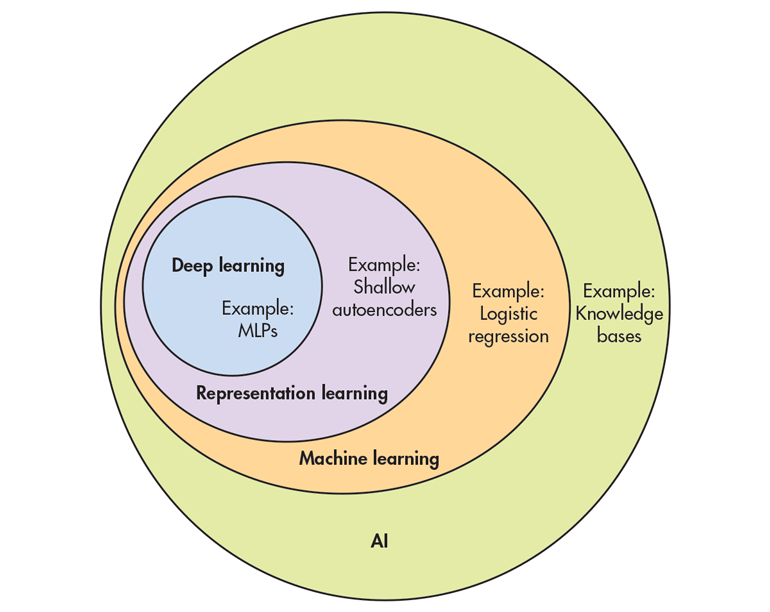
\includegraphics[width=250pt]{0}
	\centering
	\caption{The AI-ML-DL venn diagram}
\end{figure}

\section{Perceptron}

The perceptron is the basic structural building block of deep learning. A single neuron in a neural network is called a perceptron. The perceptron is typically trained using a type of algorithm called the Perceptron Learning Rule, which adjusts the weights assigned to each input based on the error between the predicted output and the true output. This process of adjusting the weights continues until the perceptron is able to accurately classify the inputs.

$$\hat{y}  = g \lt(w_0 + \sum_{i = 1}^m x_i w_i  \rt)$$

where: \\ $\hat{y} =  \textrm{Output variable}$ \\ $g = \textrm{Non linear activation function}$ \\ $w_0 =  \textrm{Bias}$ \\ $x_i = \textrm{Linear combination of input variables}$ \\ $w_i = \textrm{Weights}$

\subsection{Limitations of Linear Perceptron}
The linear perceptron is a simple and foundational model in machine learning, but it does have several limitations. Here are some of the main limitations of a linear perceptron:

\begin{enumerate}
    \item \textbf{Linear Separability}: The most significant limitation of a linear perceptron is its inability to handle non-linearly separable data. A perceptron can only learn linear decision boundaries, which means it struggles to classify data that isn't linearly separable. Non-linear patterns require more complex models to be learned accurately.
		\begin{figure}[h]
			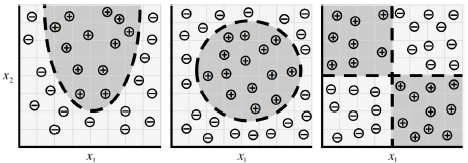
\includegraphics[width=250pt]{1}
			\centering
			\caption{Non linearities in data}
		\end{figure}

    \item \textbf{Binary Classification}: A standard linear perceptron is designed for binary classification tasks, meaning it can only classify data into two classes. It can't handle multi-class classification problems directly. Extensions like the one-vs-all or one-vs-one strategy can be used to address this limitation, but they can be less efficient and might require more resources.

    \item \textbf{Limited Representation}: The perceptron model is limited in its ability to represent complex relationships between features. It can't capture interactions between features or learn higher-level abstractions. This limitation becomes evident when dealing with tasks that involve capturing intricate patterns or relationships in the data.

    \item \textbf{Lack of Depth}: A perceptron consists of a single layer, which means it doesn't have the capacity to create deep hierarchical representations of data. Deep learning models with multiple layers have shown to be more effective in learning abstract features and complex patterns.

    \item \textbf{Convergence and Learning Rate}: The convergence of a perceptron's learning process is not guaranteed for all datasets. Some datasets may be inherently difficult to learn with a simple perceptron due to the learning algorithm's limitations. Additionally, choosing an appropriate learning rate can be challenging; if it's too high, the algorithm might not converge, and if it's too low, the learning process can be slow.

    \item \textbf{Sensitive to Feature Scaling}: The performance of a perceptron can be influenced by the scale of the input features. When features have significantly different scales, it can cause convergence issues and lead to slow learning or suboptimal results.

    \item \textbf{No Hidden Layers}: The traditional perceptron model lacks hidden layers, which means it can't learn complex feature transformations or hierarchical representations that are often necessary for more advanced tasks. Hidden layers are a crucial component of modern neural network architectures.

    \item \textbf{Limited Applications}: While the perceptron can be used for basic classification tasks, it's not well-suited for many modern machine learning applications that require handling complex data types like images, audio, and sequences. More sophisticated models, such as convolutional neural networks (CNNs) and recurrent neural networks (RNNs), are better equipped for such tasks.

    \item \textbf{Initialization Dependence}: The initial weights of the perceptron can influence its learning process and convergence. Choosing appropriate initial weights can be crucial for achieving good performance.
\end{enumerate}


Deep learning models typically consist of multiple layers of interconnected neurons, each with their own set of weights and biases, and often utilizing activation functions that are more complex than the simple step function used in perceptrons. Deep learning models typically consist of multiple layers of interconnected neurons, each with their own set of weights and biases, and often utilizing activation functions that are more complex than the simple step function used in perceptrons.

For computational convinience we denote this function in the form of a matrix multiplication of two vectors. Rewriting this equation it looks something as follows:

$$\hat{y} = g \lt( w_0 + \bs{X^T W} \rt)$$
where: $\bs{X} = \begin{bmatrix}x_1 \\ x_2 \\ \vdots \\ x_m \end{bmatrix}$
and $\bs{W} = \begin{bmatrix}w_1 \\ w_2 \\ \vdots \\ w_m \end{bmatrix}$

The $g$ in these equations is a non-linear activation function. The simplest example of non-linear activation function is a sigmoid function.

Sigmoid:

\begin{verbatim}
torch.nn.functional.sigmoid(z)
\end{verbatim}

$$g(z) = \frac{1}{(1+e^{-z})}$$
$$g'(z) = g(z)(1-g(z))$$

\begin{figure}[ht]
	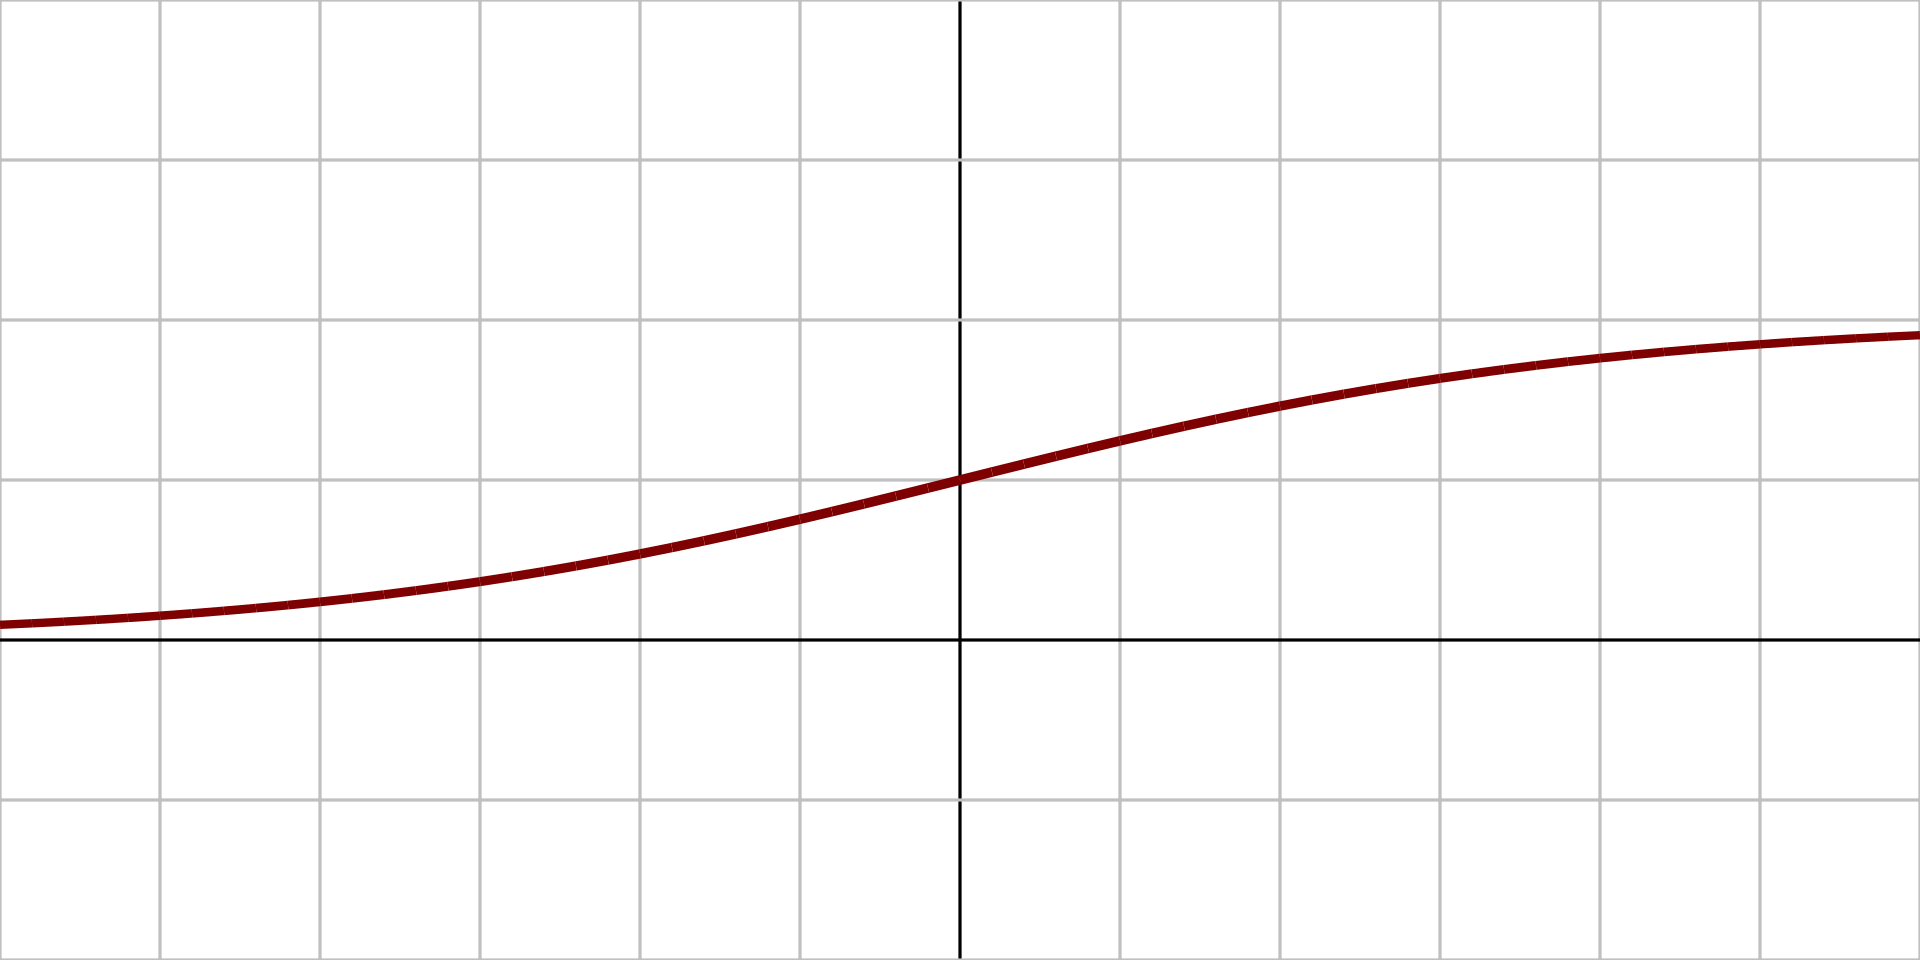
\includegraphics[width=250pt]{2}
	\centering
	\caption{Sigmoid activation function}
\end{figure}

Non-linear activation functions introduce non-linearities into the output of each neuron, allowing the network to model complex patterns in the data. This allows neural networks to learn more complex and sophisticated functions than linear models.

Some other forms of non-linear functions that are used in deep learning are hyperbolic tangent or $tanh$ and ReLU (Rectified Linear Unit)

Hyperbolic tangent:

\begin{verbatim}
torch.nn.functional.tanh(z)
\end{verbatim}

$$g(z) = \frac{e^z - e^{-z}}{e^z + e^{-z}}$$
$$g'(z) = 1 - g(z)^2$$

\begin{figure}[ht]
	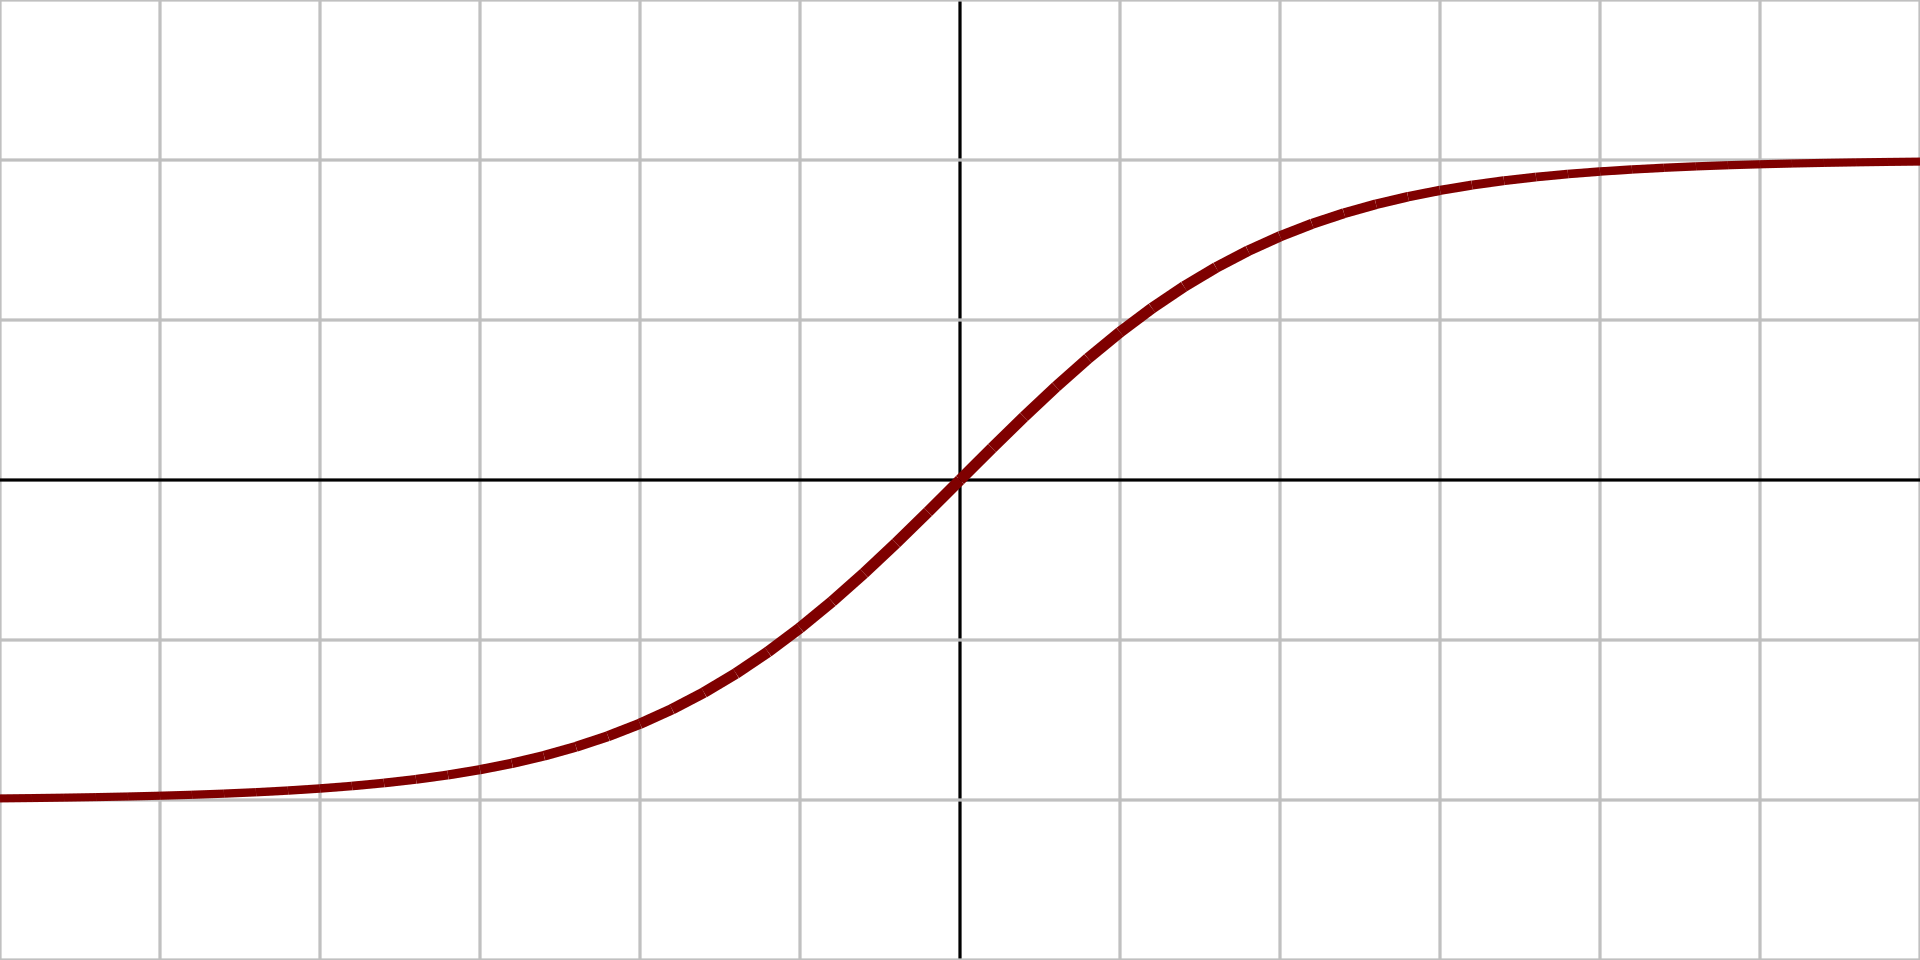
\includegraphics[width=250pt]{3}
	\centering
	\caption{tanh activation function}
\end{figure}

ReLU:
\begin{verbatim}
torch.nn.functional.relu(z)
\end{verbatim}

$$g(z) = \textrm{max}(0,z)$$
$$g'(z) =
\begin{cases}
	1, \quad z>0\\
	0, \quad \textrm{otherwize}
\end{cases}$$

\begin{figure}[ht]
	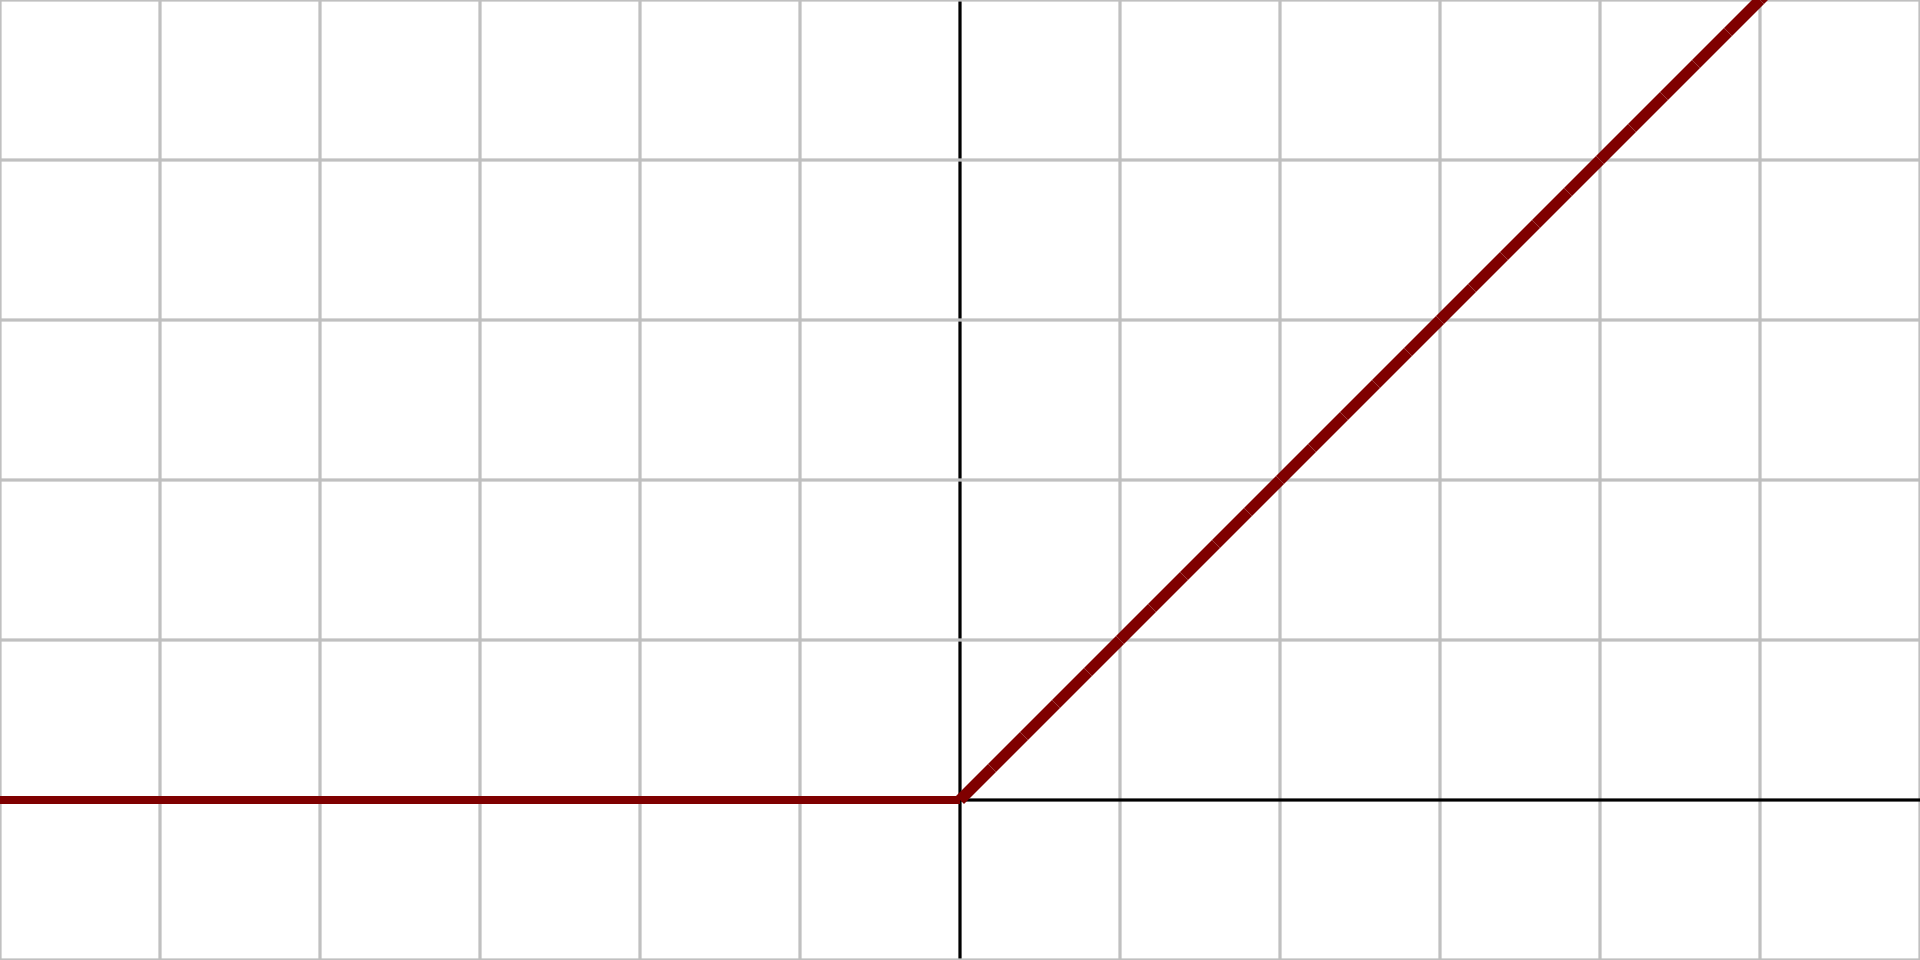
\includegraphics[width=250pt]{4}
	\centering
	\caption{ReLU activation function}
\end{figure}


We observe that the derivative of the ReLU function resolves down to a binary output. This is useful as it makes ReLU a very computationally efficient function. ReLU is a very simple activation function, computationally efficient and easy to implement. It is a threshold function that sets all negative values to zero, while passing all positive values unchanged. This is why it is the most popular activation function used in deep learning applications.

\section{Learning XOR}
XOR, short for Exclusive OR, is a logical operation that outputs true only when the number of true inputs is odd. In other words, XOR returns true if the inputs are different, and false if the inputs are the same. It is commonly represented by the symbol \(\oplus\) or \(\veebar\). The XOR operation is widely used in digital logic, boolean algebra, and computer science for various applications, including circuit design, cryptography, and data manipulation. When exactly one of these binary values is equal to 1, the XOR function returns 1. Otherwise, it returns 0.

$$X = ([0, 0]^T, [0,1]^T,[1, 0]^T,[1, 1]^T)$$
The XOR function provides the target function
$y = f^\ast(x)$ that we want to learn. Our model provides a function $y = f(x;\theta)$, and our learning algorithm will adapt the parameters $\theta$ to make $f$ as similar as possible to $f^\ast$ Considering the problem as a regression problem with a mean squared loss function, (this setup is for mathematical modeling. In practice MSE doesn't work well with binary data) Evaluating on our whole set the MSE loss function is

$$J(\theta) = \frac{1}{4}\sum_{x\in X}(f^\ast(x) - f(x;\theta))^2$$

Suppose our neural network can approximate over a linear function then our weights $\theta = [w,b]$. Thus our model is defined to be

$$f(x;w,b) = x^Tw + b$$

After solving the normal equations, we obtain $w = 0$ and $b=1/2$. The next figure shows how a linear model is not able to represent the XOR function.

\begin{figure}[ht]
	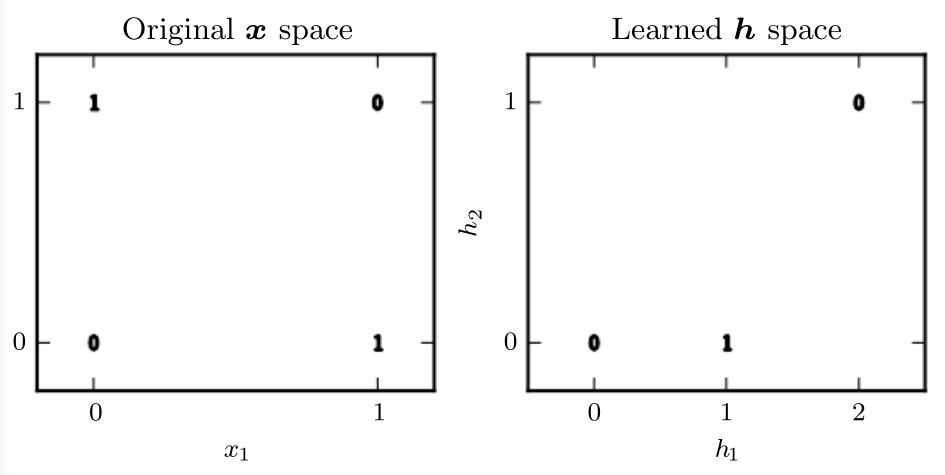
\includegraphics[width=250pt]{6}
	\centering
\end{figure}
As we observe, the model of a single percenptron fails to fit over the XOR function. Let us introduce one hideen unit $h$ that is computed by a function $f^{(1)}(x;W,c)$. The values of the hidden layer is then used for a second layer. The second layer is the output layer of the network.

The network now contains two functions chained together, h = f (1) (x; W , c) and y = f (2)(h ; w, b), with the complete model being $f(x; W , c, w , b) = f^{(2)} (f^{(1)}(x))$. With the nonlinear activation function ReLU $g = max(0,z)$ on the hyppthesis $h= g(W^Tx + c)$ we get:
$$f(x;W, c,w, b) = w^T max{0,W^Tx + c} + b$$


\begin{figure}[ht]
	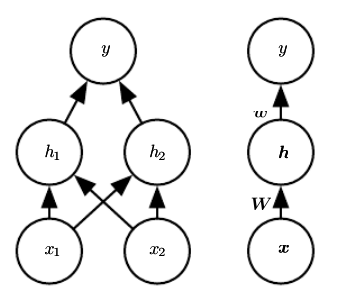
\includegraphics[width=250pt]{7}
	\centering
\end{figure}

This model finally solved the problem.

\section{Implementation of a multi-output perceptron}

Using PyTorch we can construct a dense layered multi-output perceptron by following lines of code.

\begin{verbatim}
import torch
x = torch.nn.Linear(in_features, out_features, bias=True, 
device=None, dtype=None)
\end{verbatim}

PyTorch conviniently abstracts a lot of processes which include initialization of weights and bias, Forward propogate the inputs and feed through a non-linear activation function. This would otherwize look like following

\begin{verbatim}
class MLP(nn.Module):
    def __init__(self, input_dim, hidden_dim, output_dim):
        super(MLP, self).__init__()
        self.input_layer = nn.Linear(input_dim, hidden_dim)
        self.hidden_layer = nn.Linear(hidden_dim, hidden_dim)
	    self.output_layer = nn.Linear(hidden_dim, output_dim)
        self.relu = nn.ReLU()

	def forward(self, x):
	    x = self.relu(self.input_layer(x))
	    x = self.relu(self.hidden_layer(x))
	    x = self.output_layer(x)
	    return x
\end{verbatim}

	This constructs us a single layered neural network with two outputs. In deep learning however we stack multiple such layers.

For multiple outputs, we want out output vector to be a probability distribution over a set of mutually exclusive labels. Probability distribution gives us a better idea of confidence in predictions. The softmax function is often used to predict the probabilities associated with a multinoulli distribution. Output of a neuron in a softmax layer depends on the outputs of all the other neurons in its layer and requires the sum of all the outputs to be equal to one. The softmax function is defined to be:
$$\textrm{softmax}(x)_i = \frac{\textrm{exp}(x_i)}{\sum_{j=1}^n\textrm{exp}(x_j)}$$

\section{Quantifying Loss}

A loss function represents the error or the difference between the predicted output and the actual output for a given input. The goal of machine learning is to minimize the loss, so that the model can make accurate predictions on new data.

$$L(\overbrace{f(x^{(i)})}^\textrm{predicted}; \bs{W}), \overbrace{y^{(i)}}^\textrm{actual})$$

The empirical loss measures the total loss over our entire dataset. Thus the empirical loss is the global average of all losses calculated from the predicted data. This is also called the cost function or the objective function or the empirical risk.

$$\bs{J(W)} = \frac{1}{n} \sum_{i=1}^n \lt(L(f(x^{(i)}; \bs{W}), y^{(i)})\rt)$$

The softmax cross-entropy loss is a commonly used loss function in machine learning, particularly in classification problems where the output is a probability distribution over multiple classes. The softmax cross-entropy loss penalizes the model more when it makes large errors, and encourages it to assign higher probabilities to the correct class. During training, the goal is to minimize this loss by adjusting the model's parameters.

$$L = - \sum\limits_{i=1}^n y_i \log(p_i)$$

\section{Loss Optimization by Gradient Descent}
The aim of machine learning is loss optimization and the aim of loss optimization is to minimize the loss for a given set of weights. The set of weights that achieves the minimum loss is said to be the optimal weights.

$$\bs{W^*} = \textrm{argmin} \frac{1}{n} \sum_{i = 1}^{n} \lt( L(f(x^{(i)}); \bs{W}), y^{(i)}) \rt)$$
$$\bs{W^*} = \textrm{argmin} \bs{J(W)}$$

The algorithm we solve the loss optimization problem is gradient descent. The idea behind gradient descent is to start with an initial guess for the values of the parameters, and then repeatedly update the parameters in the direction that decreases the value of the function the most. Specifically, at each iteration, the algorithm calculates the gradient of the function with respect to the parameters and then updates the parameters by subtracting a small fraction of the gradient, also known as the learning rate, from the current parameter values. The learning rate determines how big of a step the algorithm takes in each direction, and can have a significant impact on the performance of the algorithm.

\subsection{Algorithm Steps}
The steps of the gradient descent algorithm are as follows:
    
    \begin{enumerate}
        \item Initialize the model's parameters randomly or with some predefined values.
        \item Calculate the gradient of the loss function with respect to each parameter. The gradient indicates the direction of the steepest increase of the loss.
        \item Update the model's parameters by subtracting a fraction (learning rate) of the gradient from each parameter. This step is done to move the parameters in the direction that reduces the loss.
        \item Repeat steps 2 and 3 iteratively until a stopping criterion is met, such as a certain number of iterations or a small change in the loss.
    \end{enumerate}
    
\subsection{Learning Rate}
The learning rate is a hyperparameter that determines the step size taken in each iteration. A high learning rate can lead to overshooting the minimum, while a low learning rate can slow down convergence. Finding an appropriate learning rate is crucial for efficient convergence.

$$\bs{W}_{j} := \bs{W}_{j} - \eta \frac{\partial J(\bs{W}_{0},\bs{W}_{1},\ldots,\bs{W}_{n})}{\partial \bs{W}_{j}}$$

where:

$\bs{W}_{j} = $ $j$-th parameter being optimized \\ $\eta = $ learning rate (step size) \\ $J = $ cost function being minimized \\ $\frac{\partial J}{\partial \bs{W}_{j}} = $ the partial derivative of the cost function with respect to the $j$-th parameter.

The gradient descent algorithm updates the values of the parameters $\bs{W}_{j}$ at each iteration by subtracting a fraction of the gradient of the cost function with respect to that parameter.

However, for high-dimensional neural networks this gradient becomes too complex and difficult to search for the global minima. Typically the problem lies in the learning rate. Having a fixed learning rate for this application, the model may not reach the global minima. An adaptive learning rate, also known as a learning rate schedule or learning rate decay, is a technique used in machine learning optimization algorithms, such as gradient descent, to adjust the learning rate during training. Instead of using a fixed learning rate for the entire training process, the learning rate is adjusted based on certain criteria or a predetermined schedule.

Adaptive learning rates adjust the value according to how large the gradient is, how fast the learning is happening and the size of particular weights.

\subsection{Delta rule}

$\frac{\partial E}{\partial w_k} = \frac{\partial}{\partial w_k}\lt( \frac{1}{2} \sum_{i}(t^{(i)} - y^{(i)})^2\rt)$

$\frac{\partial E}{\partial w_k} =  \frac{1}{2} \sum_{i}\frac{\partial}{\partial w_k}(t^{(i)} - y^{(i)})^2$

$\frac{\partial E}{\partial w_k} = \frac{1}{2} \sum_i 2(t^{(i)} - y^{(i)}) \frac{\partial}{\partial w_k}(t^{(i)} - y^{(i)})$

$\frac{\partial E}{\partial w_k} = \sum_i (t^{(i)} - y^{(i)}) \frac{\partial}{\partial w_k}(t^{(i)} - \vec{w} \cdot \vec{x}^{(i)})$

$\frac{\partial E}{\partial w_k} = \sum_i (t^{(i)} - y^{(i)})(-x^{(i)}_k)$

$\Delta w = -\eta \frac{\partial E}{\partial w_k}$

$\Delta w = -\eta \frac{\partial}{\partial w_k}\lt( \frac{1}{2} \sum_i (t^{(i)} - y^{(i)})^2 \rt)$

$\Delta w = \sum_i \eta \lt(t^{(i)} - y^{(i)}\rt)\frac{\partial y_i}{\partial w_k}$

$\Delta w = \sum_i \eta x_k^{(i)}\lt(t^{(i)} - y^{(i)}\rt)$

Designing and training a neural network is not much different from training any other machine learning model with gradient descent. The largest difference between the linear models we have seen so far and neural networks is that the nonlinearity of a neural network causes most interesting loss functions to become nonconvex. This means that neural networks are usually trained by using iterative, gradient-based optimizers that merely drive the cost function to a very low value, rather than the linear equation solvers used to train linear regression models or the convex optimization algorithms with global conver- gence guarantees used to train logistic regression or SVMs.

\begin{figure}[ht]
	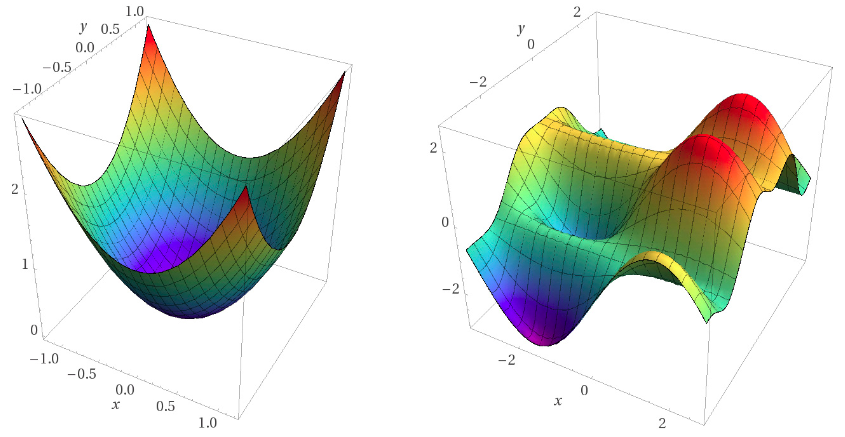
\includegraphics[width=250pt]{8}
	\centering
	\caption{An example of a convex and a non convex surface function}
\end{figure}

What makes non-convex optimization hard?
\begin{itemize}
	\item Potentially many local minima
	\item Saddle points
	\item Very flat regions or plateues
	\item Widely varying curvature
\end{itemize}

To solve non-convex problems we can concepts such as Stochastic gradient descent, Mini-batching, SVRG (stochastic variance reduced gradient), Momentum etc. There are also specialized methods for solving non-convex problems such as Alternating minimization methods, Branch-and-bound methods. These generally aren’t very popular for machine learning problems.


\section{The Vanishing Gradient Problem}
Activation functions like sigmoid shrinks a large input space into an input space between the ranges of 0 to 1. The maximum point of the function is 1/4, and the function horizontally asymptotes at 0. In other words, the output of the derivative of the cost function is always between 0 and 1/4. 

This corresponds to the effect of vanishing gradient where a large change in the input space will result in a smaller change in the output. Not only does this make the learning much slower but it also results in the "gradient vanishing" which means that the gradient is not steep enough and the model will get stuck at a platue and may not minimize the loss.

Imagine training a neural network is like traversing a landscape represented by a 3D gradient surface. The landscape has hills and valleys, where the height at any point corresponds to the value of the loss function. The goal is to find the lowest point (minimum) on this landscape. In some areas of the landscape, you encounter shallow valleys with gradual slopes. These regions correspond to parts of the parameter space where the loss changes slowly. During gradient descent, when you're in a shallow valley, the gradients (which represent the slope of the surface) are small. As a result, the updates to the model's parameters are also small. 

Now, imagine you're training a neural network with multiple layers. Each layer introduces a new hill-and-valley pattern in the landscape. As you move deeper into the network (closer to the input layer), you might encounter regions where the slopes of these hills become extremely shallow. This means that the gradients at these layers are close to zero, as they indicate how much the loss changes as you change the parameters.

When gradients become very small, updates to the model's parameters become tiny. This results in sluggish learning, where the parameters barely change during training. As a consequence, the network fails to learn meaningful features from the data, leading to poor performance. This is known as the vanishing gradient problem. To address the vanishing gradient problem, various techniques have been developed.

\subsection{Delta rule with sigmoid activation function}
$f(x) = \hat{y} = \frac{1}{1+e^{-{wx+b}}}$

Loss$(w,b) = \sum^n_{i=1}(y_i - \hat{y}_i)^2$

$\frac{\partial}{\partial w}\left(\frac{1}{1+e^{-(w x+b)}}\right) =\frac{-1}{\left(1+e^{-(w x+b)}\right)^2} \frac{\partial}{\partial w}\left(e^{-(w x+b)}\right)$

$\frac{\partial}{\partial w}\left(\frac{1}{1+e^{-(w x+b)}}\right) =\frac{-1}{\left(1+e^{-(w x+b)}\right)^2} *\left(e^{-(w x+b)}\right) \frac{\partial}{\partial w}(-(w x+b))$

$\frac{\partial}{\partial w}\left(\frac{1}{1+e^{-(w x+b)}}\right) =\frac{-1}{\left(1+e^{-(w x+b)}\right)} * \frac{e^{-(w x+b)}}{\left(1+e^{-(w x+b)}\right)} *(-x)$

$\frac{\partial}{\partial w}\left(\frac{1}{1+e^{-(w x+b)}}\right) =\frac{1}{\left(1+e^{-(w x+b)}\right)} * \frac{e^{-(w x+b)}}{\left(1+e^{-(w x+b)}\right)} *(x)$

$\frac{\partial}{\partial w}\left(\frac{1}{1+e^{-(w x+b)}}\right) =f(x) *(1-f(x)) * x$

$\Delta w = \frac{\partial}{\partial w}\lt[ \frac{1}{2} \cdot (f(x) - y)^2\rt]$

$\Delta w = \frac{1}{2} \cdot \lt[2 \cdot (f(x) - y) \cdot \frac{\partial}{\partial w}(f(x) - y)\rt]$

$\Delta w = (f(x) - y) \cdot \frac{\partial}{\partial w}f(x)$

$\Delta w = (f(x) - y) \cdot \frac{\partial}{\partial w}\lt(\frac{1}{1 + e^{-wx+b}}\rt)$

$\Delta w = (f(x)-y) \overbrace{f(x) \cdot (1-f(x)) \cdot x}^\textrm{sigmoid derivative}$

\section{Backpropogration}
Backpropagation is a key algorithm used to train neural networks through supervised learning. It involves calculating the gradient of the loss function with respect to the model's parameters, which is then used to update the parameters in the direction that reduces the loss. The process involves two main phases: forward propagation and backward propagation.
    
\subsection{Forward Propagation}
    
    During forward propagation, input data is fed into the network, and activations are computed layer by layer. Each layer applies a linear transformation (weighted sum) followed by an activation function. The final output of the network is produced.
    
\subsection{Backward Propagation}
    
    Backward propagation involves computing the gradient of the loss function with respect to the output of each layer. This is done recursively by applying the chain rule of calculus. The gradient is propagated backward through the layers, allowing the calculation of gradients for the parameters of each layer.
    
\subsection{Update Rule}
    
    The update rule for each parameter during training can be expressed using the gradient of the loss function (\(\nabla\) denotes the gradient operator):
    
    \[ \text{New parameter value} = \text{Old parameter value} - \text{learning rate} \times \nabla \text{Loss w.r.t. parameter} \]
    
    
    The equation for updating a parameter \(w\) using gradient descent can be represented as:
    
    \[ w_{\text{new}} = w_{\text{old}} - \text{learning rate} \times \frac{\partial \text{Loss}}{\partial w} \]
    
    Where:
    \( w_{\text{new}} \) is the new value of the parameter,
    \( w_{\text{old}} \) is the old value of the parameter,
    \(\frac{\partial \text{Loss}}{\partial w}\) is the gradient of the loss with respect to the parameter \(w\).
    
    The forward and backward propagation steps, followed by parameter updates, are repeated iteratively until the loss converges or a maximum number of iterations is reached.

\section{Stochastic Gradient Descent and Mini batches}
Stochastic gradient descent (SGD) is an iterative optimization algorithm used to minimize the cost function in machine learning models. It is an extension of gradient descent, a more traditional optimization algorithm that updates the model parameters based on the average gradient of the entire dataset.

In contrast, stochastic gradient descent updates the model parameters based on the gradient of a randomly selected subset (or mini-batch) of the training data. This random selection introduces stochasticity into the algorithm, which can help it escape from local optima and converge more quickly.

By this method, instead of computing the gradient over an entire dataset we compute a gradient over a small batch. This estimate of the gradient is very noisy however it produces a smoother convergence and allows larger learning rates while being computationally inexpensive. Furthermore these mini-bactches can be computed in clusters. This parallelization of loss optimization has made deep learning over an astronomically large dataset possible.

The negative conditional log-likelihood of the training data can be written as

$$
J(\boldsymbol{\theta})=\mathbb{E}_{\mathbf{x}, \mathbf{y} \sim \hat{p}_{\mathrm{data}}} L(\boldsymbol{x}, y, \boldsymbol{\theta})=\frac{1}{m} \sum_{i=1}^m L\left(\boldsymbol{x}^{(i)}, y^{(i)}, \boldsymbol{\theta}\right)
$$
where $L$ is the per-example loss $L(\boldsymbol{x}, y, \boldsymbol{\theta})=-\log p(y \mid \boldsymbol{x} ; \boldsymbol{\theta})$

Specifically, on erac h step of the algortithm we can sample a minibatch of example $B = \lt(x^{(i)}, \cdots , x^{(m)}\rt)$ drawn uniformly from a training set. The minibatch size m in typically chosen to be a relatively small number of examples. The estimate of the gradient formed is

$$J(\theta) = \frac{1}{m} \nabla \theta \sum_{i=1}^m L(x^{(i)}, y^{(i)}, \theta)$$

Using examples from minibarch B, The stochastic gtradient descent algorithm then follows the estimated gradient downhill.

\section{Capacity, Overfitting and Underfitting}
The central objective of machine learning is to learn from data provided and in turn predict well on new and unseen inputs. The ability of performing well on unobserved data is called generalization. The factors determining how well a machine learning algortihm will perform are its ability to:
\begin{enumerate}
	\item Make the training error small 
	\item Make the gap between the training and tesing error small.
\end{enumerate}

\begin{figure}[ht]
	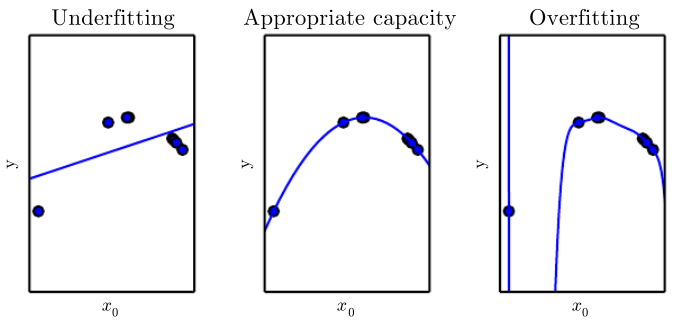
\includegraphics[width=250pt]{5}
	\centering
\end{figure}

\textbf{Underfitting} occurs when the model is not able to obtain a sufficiently low error value on the training set.  \textbf{Overfitting} occurs when the gap between the training error and test error is too large. We can control whether a model is more likely to overfit or underfit by altering its \textbf{Capacity}.

A model's capacity is its ability to fit a wide variety of functions. Models with low capacity may struggle to fit the training set while the models with high capacity can overfit by memorizing properties of the training set.

There are several methods by which overfitting can be avoided in deep neural networks like regularization, dropout, data augmentation and early stopping.

\section{Regularization}
Because neural networks are extremely large models they are very prone to overfitting. Techniques of regularization has implications towards success of neural networks. The most popular technique of regularization in deep learning is called dropout. Dropout is a regularization method that approximates training a large number of neural networks with different architectures in parallel.

During training, some number of layer outputs are randomly ignored or “dropped out.” This has the effect of making the layer look-like and be treated-like a layer with a different number of nodes and connectivity to the prior layer. In effect, each update to a layer during training is performed with a different “view” of the configured layer.


Another way of preventing overfitting is a technique in regularization of early stopping. Since the problem of overfitting is when the model starts to represent the training data more than the testing data, we can look at the trends of training and testing accuracy druing the training of the model and stop the training as soon as the testing accuracy starts to reduce.

\chapter{Developments in Deep Learning}

\section{Softmax and Negative Log Likelihood}
The cross-entropy between two probability distributions $p$ and $q$ over the same underlying set of events measures the average number of bits needed to identify an event drawn from the set if a coding scheme used for the set is optimized for an estimated probability distribution $q$, rather than the true distribution $p$.

The cross-entropy of the distribution $q $relative to a distribution $p$ over a given set is defined as follows:
$$H(p,q) = -E_p[log q]$$
where $E_{p}[\cdot ]$ is the expected value operator with respect to the distribution $p$. Using cross-entropy in the cost function.

\subsection{Softmax}

The softmax activation function is often placed at the output layer of a neural network. It’s commonly used in multi-class learning problems where a set of features can be related to oneof K  classes. For example, in the CIFAR-10 image classification problem, given a set of pixels as input, we need to classify if a particular sample belongs to one-of-ten available classes: i.e., cat, dog, airplane, etc. Its equation is simple, we just have to compute for the normalized exponential function of all the units in the layer. In such case,

$$S(f_{y_i}) = \frac{e^{f_{y_i}}}{\sum_j e^{f_j}}$$

Intuitively, what the softmax does is that it squashes a vector of size $K$ between 0 and 1. Furthermore, because it is a normalization of the exponential, the sum of this whole vector equates to 1. We can then interpret the output of the softmax as the probabilities that a certain set of features belongs to a certain class.

Thus, given a three-class example below, the scores $y_i$ are computed from the forward propagation of the network. We then take the softmax and obtain the probabilities as shown:

\begin{figure}[ht]
	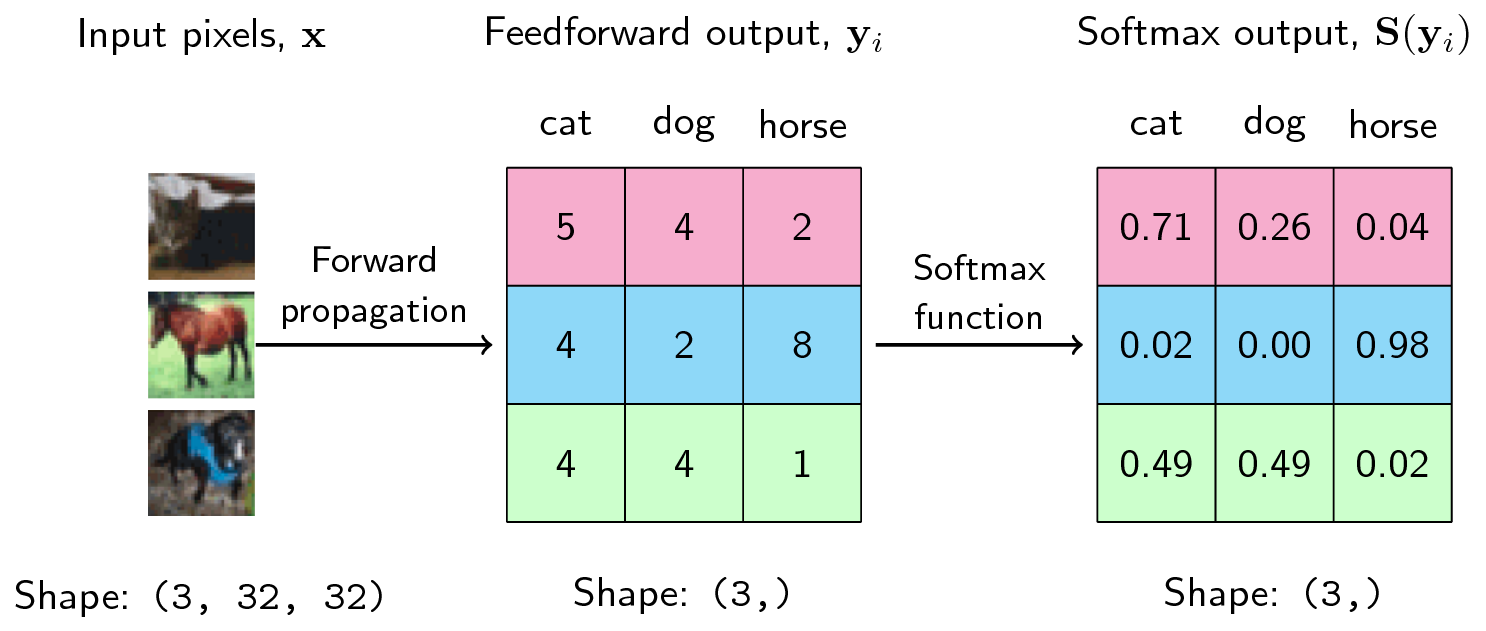
\includegraphics[width=250pt]{9}
	\centering
	\caption{Softmax Computation for three classes}
\end{figure}

The output of the softmax describes the probability (or if you may, the confidence) of the neural network that a particular sample belongs to a certain class. Thus, for the first example above, the neural network assigns a confidence of 0.71 that it is a cat, 0.26 that it is a dog, and 0.04 that it is a horse. The same goes for each of the samples above.

We can then see that one advantage of using the softmax at the output layer is that it improves the interpretability of the neural network. By looking at the softmax output in terms of the network’s confidence, we can then reason about the behavior of our model.

\subsection{Negative Log Likelihood}
In practice, the softmax function is used in tandem with the negative log-likelihood (NLL). This loss function is very interesting if we interpret it in relation to the behavior of softmax. First, let’s write down our loss function:

$$L(y) = -log(y)$$

This is summed for all the correct classes.

Recall that when training a model, we aspire to find the minima of a loss function given a set of parameters (in a neural network, these are the weights and biases). We can interpret the loss as the “unhappiness” of the network with respect to its parameters. The higher the loss, the higher the unhappiness: we don’t want that. We want to make our models happy.

So if we are using the negative log-likelihood as our loss function, when does it become unhappy? And when does it become happy? Let’s try to plot its range:

\begin{figure}[h]
	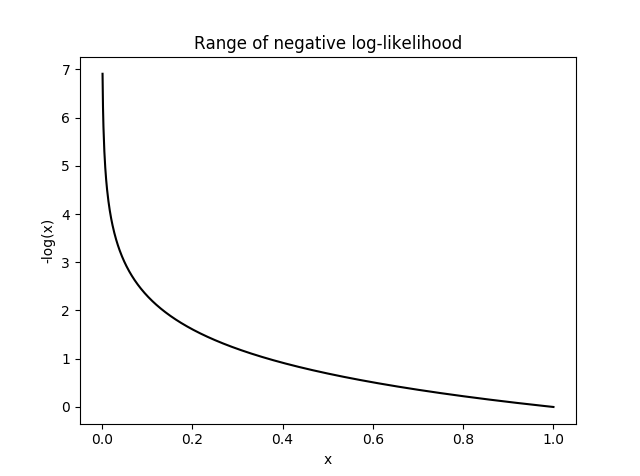
\includegraphics[width=250pt]{10}
	\centering
	\caption{The loss function reaches infinity when input is 0, and reaches 0 when input is 1.}
\end{figure}

\clearpage
\begin{figure}[ht]
	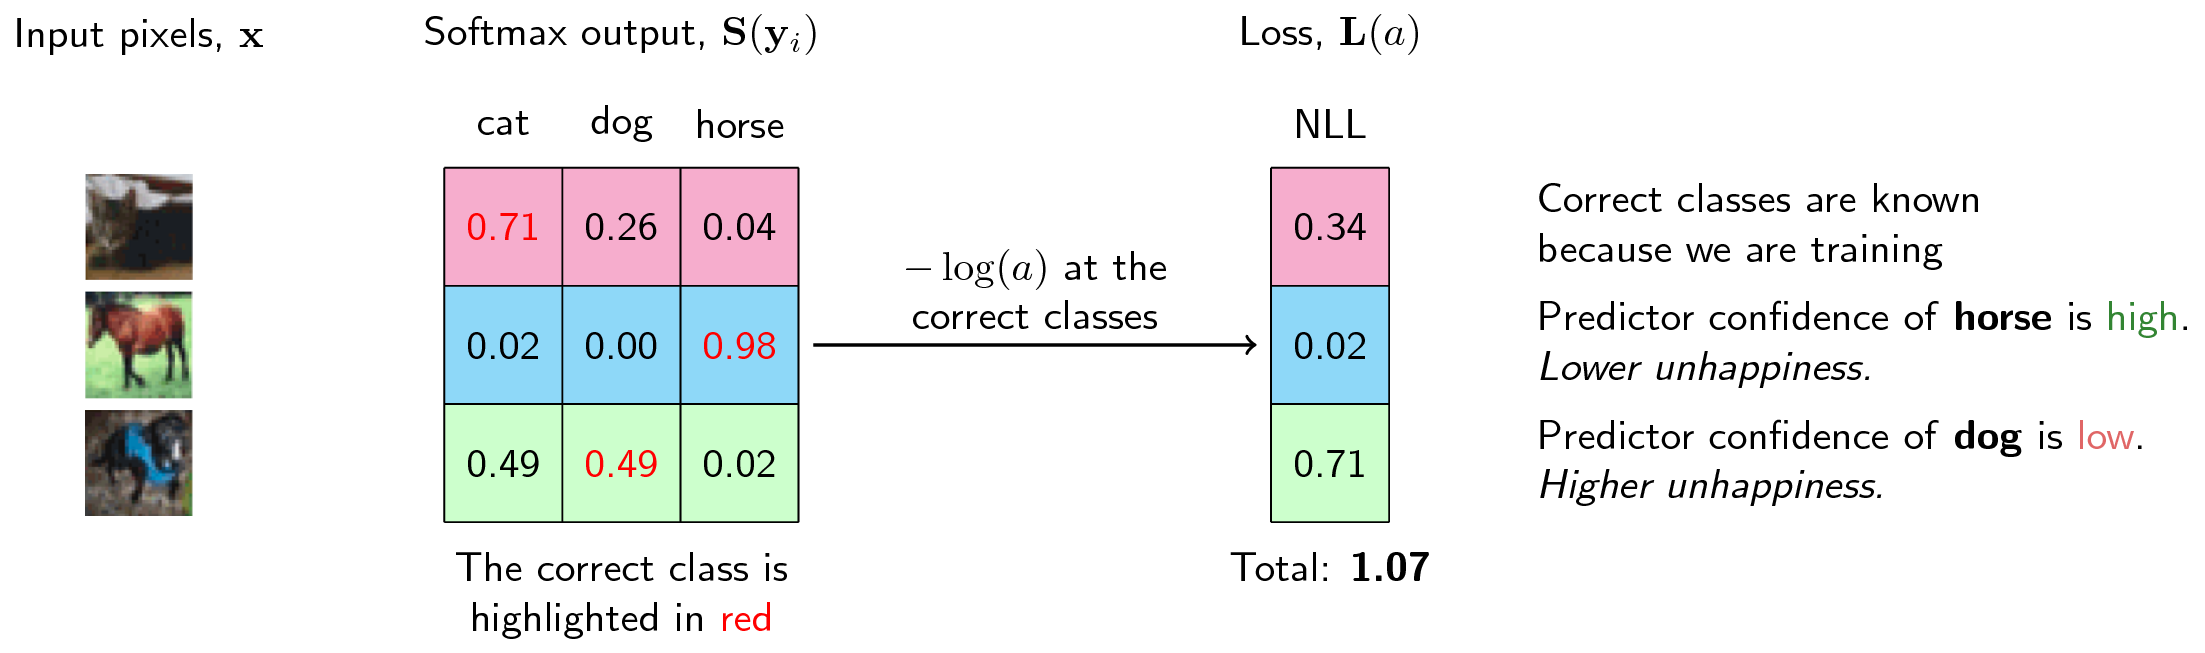
\includegraphics[width=350pt]{11}
	\centering
	\caption{When computing the loss, we can then see that higher confidence at the correct class leads to lower loss and vice-versa.}
\end{figure}
The negative log-likelihood becomes unhappy at smaller values, where it can reach infinite unhappiness (that’s too sad), and becomes less unhappy at larger values. Because we are summing the loss function to all the correct classes, what’s actually happening is that whenever the network assigns high confidence at the correct class, the unhappiness is low, but when the network assigns low confidence at the correct class, the unhappiness is high.


\subsection{Derivative of the Softmax}
Let $f$ as a vector containing the class scores for a single example, that is, the output of the network. Thus $f_k$ is an element for a certain class $k$ in all $j$ classes. We can then rewrite the softmax output as

$$p_k = \frac{e^{f_k}}{\sum_j e^{f_j}}$$

and the negative log-likelihood as

$$L_i = -log(y_{y_i})$$

when performing backpropagation, the first thing we have to do is to compute how the loss changes with respect to the output of the network. Thus, we are looking for $\frac{\partial L_i}{\partial p_k}$ and $\frac{\partial p_{y_i}}{\partial f_k}$. Via chain rule:

$$\frac{\partial L_i}{\partial f_k} = \frac{\partial L_i}{\partial p_k}\cdot \frac{\partial p_k}{\partial f_k}$$

$$\frac{\partial L_i}{\partial p_k} = \frac{1}{p_k}$$

Let the derivative be represented by the operator $\mathbf{D}$

$$\frac{f(x)}{g(x)} = \frac{g(x) \mathbf{D} f(x) - f(x) \mathbf{D} g(x)}{g(x)^2}$$

We let $\sum_j e^{f_{y_j}} = \Sigma$, and by substituting, we obtain

$$\frac{\partial p_k}{\partial f_k} = \frac{\partial}{\partial f_k} \lt( \frac{e_{f_k}}{\sum_k e^{f_{y_j}}}\rt)$$
$$ = \frac{\Sigma \mathbf{D}e^{f_k} - e^{f_k} \mathbf{D}\Sigma}{\Sigma^2}$$
$$\frac{\partial p_k}{\partial f_k} = \frac{e_{f_k}(\Sigma - e^{f_k})}{\Sigma^2}$$
$$= p_k \ast (1 - p_k)$$

$$\frac{\partial L_i}{\partial f_k} = \frac{\partial L_i}{\partial p_k}\cdot \frac{\partial p_k}{\partial f_k}$$
$$= -\frac{1}{p_k}(p_k \ast (1-p_k))$$
$$= p_k - 1$$

And thus we have differentatied the negative log likelihood with respect to the softmax layer.

\section{Hidden Units}
The design of hidden units in neural networks is a dynamic and continuously evolving field of research. Hidden units are the building blocks of neural network architectures, responsible for capturing and representing complex patterns within the data. However, despite the substantial progress in neural network research, there isn't a universally accepted set of theoretical principles that definitively guide the design of these hidden units.

Neural network researchers and practitioners frequently experiment with various activation functions and architectures to optimize the performance of their networks for specific tasks. This experimentation is driven by empirical observations rather than strict theoretical guidelines. This lack of definitive guiding principles in the design of hidden units stems from the complexity of neural networks and the intricate nature of the relationships they learn from data.

One type of activation function that has gained significant popularity is the Rectified Linear Unit (ReLU). ReLUs are considered an excellent default choice due to their simplicity and effectiveness. A ReLU activation function simply outputs the input if it's positive, and zero otherwise. Mathematically, a ReLU activation \(f(x)\) is defined as:

$f(x) = \max(0, x)$

ReLUs have several advantages that make them a preferred choice in many scenarios. They are computationally efficient to compute, they help mitigate the vanishing gradient problem by allowing gradients to flow freely during backpropagation, and they have been empirically shown to work well for a wide range of tasks, including image recognition and natural language processing.

While ReLUs offer several benefits, it's important to note that there's no one-size-fits-all solution in neural network architecture design. Depending on the specific problem, data characteristics, and network architecture, other activation functions like sigmoid, tanh, or variants of ReLU (such as Leaky ReLU and Parametric ReLU) might also be considered. Experimentation and empirical validation play a crucial role in selecting the most appropriate activation functions and hidden unit designs for a given task.

Other hidden units to choose from are:
\begin{itemize}
	\item signmoid
	\item tanh
	\item Radial basis function
	\item Softplus
	\item Hard tanh
\end{itemize}

\section{Architecture Design: Key Considerations}

Designing neural networks involves making critical decisions about the architecture of the network, including the number of units (neurons) and how these units are interconnected. These decisions greatly influence the network's capacity to learn and generalize from data. Two fundamental architectural considerations are the depth of the network and the width of each layer.

The depth of a neural network refers to the number of layers it contains. Deeper networks have more layers, and each layer is responsible for extracting and representing different levels of features from the input data. As data flows through the layers, the network captures increasingly complex patterns and abstractions. However, adding more layers doesn't always guarantee better performance. Very deep networks might suffer from vanishing gradients, making them difficult to train. On the other hand, deep architectures like convolutional neural networks (CNNs) and transformers have demonstrated remarkable success in tasks like image recognition and natural language processing.

The width of a layer in a neural network corresponds to the number of units or neurons within that layer. A wider layer has more neurons, allowing it to capture more diverse and detailed features. A narrower layer, on the other hand, reduces the number of parameters and computational complexity. The choice of layer width depends on factors such as the complexity of the task, the amount of available data, and computational resources. In practice, increasing the width of layers can improve a network's capacity to memorize the training data but might also increase the risk of overfitting.

The architectural decisions regarding the depth and width of a neural network often involve a trade-off. Deep networks with narrow layers can be computationally expensive and prone to overfitting if not properly regularized. Shallower networks with wider layers might be computationally efficient but might not capture as intricate patterns. Achieving the right balance between depth and width is a crucial aspect of neural network design.

Due to the absence of strict theoretical guidelines for determining the optimal depth and width of a network, practitioners often rely on empirical exploration and experimentation. Techniques like cross-validation, regularization, and network architecture search are commonly used to identify architectures that perform well on specific tasks.

In general, a feedforward network with a single layer is sufficient to represent any function, but the layer may be infeasibly large and may fail to learn and generalize correctly. 
In many circumstances, using deeper models can reduce the number of units required to represent the desired function and can reduce the amount of generalization error.

\section{Universal Approximation Theorem}

The process of learning a nonlinear function often requires the design of a specialized model that can capture complex relationships within the data. Feedforward neural networks with hidden layers provide a powerful framework for achieving this. The \textbf{universal approximation theorem} asserts that feedforward networks with at least one hidden layer and an appropriate activation function can approximate any Borel measurable function from one finite-dimensional space to another. This theorem underlines the capacity of neural networks to approximate a wide range of functions.

Mathematically, a feedforward neural network aims to find a function \(y = f(x)\) that maps input attributes \(x\) to output \(y\). The accuracy of this mapping varies based on the dataset distribution and the network architecture employed. The function \(f(x)\) can be highly complex, allowing the network to represent intricate patterns.

The \textbf{Universal Approximation Theorem} assures us of the universality of neural networks. Regardless of the nature of \(f(x)\), there exists a network configuration that can closely approximate the desired outcome, effectively performing the task at hand. This theorem holds true for any number of inputs and outputs.

The universal approximation theorem means that regardless of what function we are trying to learn, we know that a large MLP will be able to represent this function. However, we are not guaranteed that the training algorithm will be able to learn that function The reasons for this is that the optimization algorithm used for training may not be able to find the value of the parameters. It is also possible that the training algorithm might choose the wrong function due to overfitting. The universal approximation theorem says that there exists a network large enough to achieve any degree of accuracy we desire.

\section{Beyond Gradient Descent}
The primary challenge in optimizing deep learning models is that we are forced to use minimal local information to infer the global structure of the error surface. One observation about deep neural networks is that their error surfaces are guaranteed to have a large—and in some cases, an infinite—number of local minima. Within a layer of a fully-connected feed-forward neural network, any rearrangement of neurons will still give you the same final output at the end of the network. \textbf{A model is said to be identifiable} if a sufficiently large training set can rule out all but one setting of the model’s parameters.

Within a layer with $n$ neurons, there are $n!$ ways to rearrange parameters. And for a deep network with $l$ layers, each with $n$ neurons, we have a total of $n!l$ equivalent configurations. Within a layer with $n$ neurons, there are $n!$ ways to rearrange parameters. And for a deep network with $l$ layers, each with $n$ neurons, we have a tota$l$ of $n!l$ equivalent configurations.

Local minima are only problematic when they are spurious. A \textbf{spurious local} minimum corresponds to a configuration of weights in a neural network that incurs a higher error than the configuration at the global minimum. If these kinds of local minima are common, we quickly run into significant problems while using gradient based optimization methods.

\textbf{Flat regions} are where the gradient approaches zero. ($\nabla = 0$) This point is not a local minima, so it is unlikely to get us completely stuck. The zero gradient might slow down learning if we are unlucky enough to encounter it. A point at which the gradient is the zero vector is called a \textbf{critical point}.

Sometimes we need to find all the partial derivatives of a function whose input and output are both vectors. The matrix containing all such partial derivatives is known as a \textbf{Jacobian matrix}. Specifically, if we have a function $f : \mathbf{R}^m \rightarrow \mathbf{R}^n$, then the Jacobian matrix $J \in \mathbf{R}^{m \times n}$ of $f$ is defined such that $J_{i,j} = \frac{\partial}{\partial x_j}f(x)_i$

We are also sometimes interested in the second derivative. For example, for a function $f : \mathbf{R}^n \rightarrow \mathbf{R}$, the derivative with respect to $x_i$ of the derivative of $f$ with respect to $x_j$ is denoted as $\frac{\partial^2}{\partial x_i \partial x_j}f$. The second derivative tells us how the first derivative will change as we vary the input. This is important because it tells us whether a gradient step will cause as much of an improvement as we would expect based on the gradient alone. We can think of the second derivative as measuring curvature.

When our function has multiple input dimensions, there are many second derivatives. These derivatives can be collected together into a matrix called the \textbf{Hessian matrix}. The Hessian matrix $H(f(x))$ is defined such that

$$
H(f(x))=\left[\begin{array}{ccc}
\frac{\delta^2 f}{\delta x^2} & \frac{\delta^2 f}{\delta x \delta y} & \frac{\delta^2 f}{\delta x \delta z} \\
\frac{\delta^2 f}{\delta y \delta x} & \frac{\delta^2 f}{\delta y^2} & \frac{\delta^2 f}{\delta y \delta z} \\
\frac{\delta^2 f}{\delta z \delta x} & \frac{\delta^2 f}{\delta z \delta y} & \frac{\delta^2 f}{\delta z^2}
\end{array}\right]
$$
Rules for Maxima and Minima for a Univariate Function:
\begin{enumerate}
	\item The derivative of $f(x)$ with respect to $x$ would be zero at maxima and minima. 
	\item The second derivative of $f(x)$, which is nothing but the derivative of the first, needs to be investigated at the point where the first derivative is zero. 
	\item If the second derivative is less than zero, then it’s a point of maxima, while if it is greater than zero it’s a point of minima.  
	\item If the second derivative turns out to be zero as well, then the point is called a point of inflection. 
\end{enumerate}

\begin{figure}[ht]
	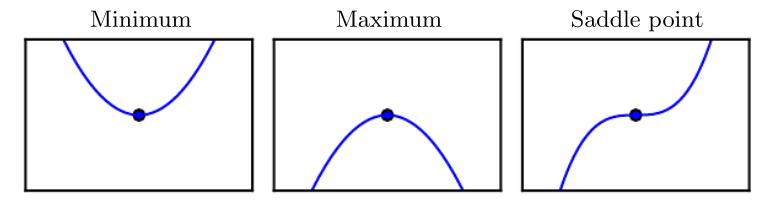
\includegraphics[width=250pt]{12}
	\centering
\end{figure}

\begin{figure}[ht]
	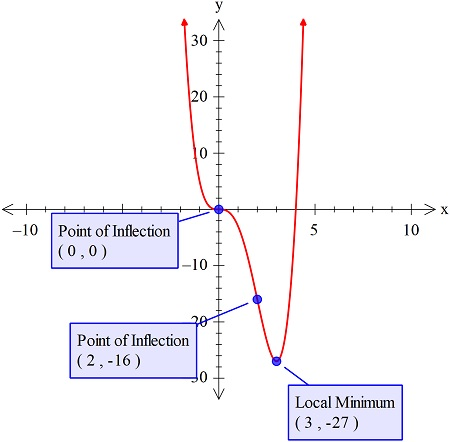
\includegraphics[width=250pt]{13}
	\centering
	\caption{Typical example of a univariate non-convex function $f(x) = x^4 + 4x^3$}
\end{figure}

\subsection{Momentum Based Optimization}

Momentum-based optimization is a variant of gradient descent, an iterative optimization algorithm used to train neural networks and other machine learning models. The core idea behind momentum-based optimization is to introduce a momentum term that helps accelerate the convergence of the optimization process, especially when the loss surface is characterized by flat regions, narrow valleys, or noisy gradients.

Traditional gradient descent can exhibit slow convergence in certain scenarios. For example, in regions of the loss surface where the gradient is small (shallow valleys) or when the gradients are noisy, the updates to the model's parameters can be small and inefficient. Additionally, gradient descent might oscillate back and forth in narrow valleys, leading to slow progress towards the optimal solution.

\begin{figure}[ht]
	
\includegraphics[width=100pt]{19}
	\centering
	\caption{Momentum Demonstration at https://distill.pub/2017/momentum/}
\end{figure}

The motivation behind introducing momentum is to address these issues and achieve faster convergence. The concept is inspired by physical principles: think of the optimization process as a ball rolling down a hill (the loss surface). If the ball encounters flat or noisy terrain, it might lose speed and slow down. Momentum introduces a "velocity" term that accumulates the historical gradients and propels the ball forward with greater force, helping it traverse through flat regions and narrow valleys more efficiently.

\textbf{Mathematical Explanation}:

In momentum-based optimization, the update rule for a parameter \(w\) incorporates the gradient of the loss as well as a "velocity" term:

$$\text{update}_{t} = \gamma \cdot \text{update}_{t-1}+\eta \nabla w_{t}$$
$$w_{t+1}=w_{t} - \text{update}_{t}$$

$$\text{or}$$

$$ \text{Velocity}_\text{new} = \gamma \times \text{Velocity}_\text{old} + \text{Learning Rate} \times \nabla \text{Loss} $$
$$ w_\text{new} = w_\text{old} - \text{Velocity}_\text{new} $$

Here, \(\gamma\) is the momentum hyperparameter that determines the influence of the historical velocity or in other terms the "friction". A higher \(\gamma\) places more emphasis on the accumulated history of gradients, allowing the optimization to navigate challenging regions more effectively.

The momentum-based optimization enhances traditional gradient descent by incorporating a momentum term that helps the optimization process to better navigate flat, noisy, or narrow regions of the loss surface. This leads to faster convergence and more efficient training of neural networks and other machine learning models.

$$\text{update}_0 = 0$$
$$\text{update}_1 = \gamma \cdot \text{update}_0 + \eta\nabla w_1 = \eta\nabla w_1$$
$$\text{update}_2 = \gamma \cdot \text{update}_1 + \eta\nabla w_2 = \gamma \cdot \eta\nabla w_1 + \eta\nabla w_2$$
$$\text{update}_3=\gamma\cdot \text{update}_2+\eta\nabla w_3=\gamma(\gamma\cdot\eta\nabla w_1+\eta\nabla w_2)+\eta\nabla w_3$$
$$=\gamma\cdot \text{update}_{2}+\eta\nabla w_{3}=\gamma^{2}\cdot\eta\nabla w_{1}+\gamma\cdot\eta\nabla w_{2}+\eta\nabla w_{3}$$
$$\text{update}_{4}=\gamma\cdot \text{update}_{3}+\eta\nabla w_{4}=\gamma^{3}\cdot\eta\nabla w_{1}+\gamma^{2}\cdot\eta\nabla w_{2}+\gamma\cdot\eta\nabla w_{3}+\eta\nabla w_{4}\,$$

$$\text{update}_{t}=\gamma\cdot \text{update}_{t-1}+\eta\nabla w_{t}=\gamma^{t-1}\cdot\eta\nabla w_{1}+\gamma^{t-2}\cdot\eta\nabla_{-}w_{1}+\ldots+\eta\nabla w_{t}$$

\subsection{Nestrov Accelerated Gradient Optimization}
Nesterov Accelerated Gradient (NAG) optimization is an enhancement of the traditional gradient descent algorithm, designed to accelerate convergence in training neural networks and other machine learning models. NAG combines the benefits of momentum-based optimization with a correction term that helps the optimization process converge more efficiently, especially in regions with steep or curved gradients.

Standard momentum-based optimization, while effective in many cases, can still exhibit slow convergence when it comes to navigating the loss surface in the presence of steep or curved gradients. In these scenarios, traditional momentum might lead to overshooting the optimal solution or struggling to accurately adjust the momentum direction.

The motivation behind Nesterov Accelerated Gradient optimization is to address this issue by introducing a "lookahead" mechanism. Instead of calculating the gradient at the current parameter values, NAG estimates the future parameter values that would result from applying momentum. This lookahead helps to better align the momentum direction with the actual trajectory of the optimization process, resulting in more accurate updates and faster convergence.

\textbf{Mathematical Explanation}:

In Nesterov Accelerated Gradient optimization, the update rule involves two steps: a lookahead step and an actual update step.

1. Lookahead Step:
\[ \text{Lookahead} = \text{Parameter}_\text{old} + \gamma \times \text{Momentum}_\text{old} \]
Here, \(\gamma\) is the momentum hyperparameter.

2. Actual Update Step:
\[ \text{Update} = \text{Parameter}_\text{old} - \text{Learning Rate} \times \nabla \text{Loss}(\text{Lookahead}) \]
Here, the gradient is calculated using the lookahead parameter values.

The lookahead mechanism provides a more accurate estimation of the gradient direction, resulting in more precise updates that are well-aligned with the true trajectory of the optimization process. This allows NAG to converge more efficiently in the presence of steep gradients, leading to faster training of neural networks.

\textbf{Advantages}:

Nesterov Accelerated Gradient optimization offers several advantages:
- Improved convergence speed in regions with steep or curved gradients.
- Reduced oscillations during optimization, leading to smoother convergence.
- Enhanced stability and robustness of the optimization process.

The Nesterov Accelerated Gradient optimization enhances traditional momentum-based optimization by introducing a lookahead mechanism, which helps the optimization process converge more efficiently, particularly in challenging regions of the loss surface.

\subsection{AdaGrad (Adaptive Gradient Algorithm)}
Adagrad, short for Adaptive Gradient Algorithm, is an optimization algorithm designed to adjust the learning rate of each parameter during the training process. It adapts the learning rate for each parameter based on the historical gradient information. Adagrad is particularly useful when dealing with data that has sparse gradients or requires different learning rates for different parameters.

In traditional gradient descent, a single learning rate is applied to all parameters of the model. However, different parameters might have different characteristics and require different learning rates for optimal convergence. For example, some parameters might have frequent updates (large gradients), while others might have infrequent updates (small gradients).

The motivation behind Adagrad is to address this issue by dynamically adapting the learning rates of each parameter based on their historical gradient magnitudes. Parameters that have been updated less frequently will receive a larger learning rate to help them converge more effectively, while parameters that have been updated more frequently will receive a smaller learning rate to prevent them from oscillating around the optimal solution.

\textbf{Mathematical Explanation}:

Adagrad maintains a separate learning rate for each parameter \(w_i\), denoted as \(G_{ii}\), which is the sum of squared gradients up to that point:

\[ G_{ii} = G_{ii} + (\nabla \text{Loss}(\theta_i))^2 \]

Here, \(\nabla \text{Loss}(\theta_i)\) is the gradient of the loss with respect to the parameter \(w_i\).

The update rule for each parameter using Adagrad is then given by:

\[ w_i^\text{new} = w_i^\text{old} - \frac{\text{Learning Rate}}{\sqrt{G_{ii} + \epsilon}} \times \nabla \text{Loss}(\theta_i) \]

Where \(\epsilon\) is a small constant added for numerical stability to prevent division by zero.

\textbf{Advantages}:

Adagrad offers several advantages:
- Automatically adapts learning rates based on historical gradients.
- Well-suited for sparse data and unevenly distributed gradients.
- Requires minimal manual tuning of learning rates.

\textbf{Considerations}:

While Adagrad is effective, it may have issues with very large gradients, causing learning rates to become too small. This led to the development of variants like Adadelta and RMSProp, which further improve upon Adagrad's adaptive learning rate scheme.

Adagrad is an optimization algorithm that adaptively adjusts learning rates for each parameter based on historical gradient information. Its motivation lies in providing a more efficient and adaptive learning rate strategy that addresses the challenges of diverse parameter characteristics and sparse gradients.

\subsection{AdaDelta}
Adadelta is an optimization algorithm designed as an improvement over Adagrad. It addresses some of the limitations of Adagrad, such as the need for manual tuning of learning rates and potential issues with very large gradients. Adadelta dynamically adjusts the learning rates using a more refined approach that helps achieve stable convergence.

While Adagrad adapts learning rates based on historical gradient information, it accumulates the sum of squared gradients in the denominator. Over time, this accumulation can cause the learning rates to shrink, making it difficult for the algorithm to make meaningful updates. Additionally, Adagrad's reliance on the historical sum of squared gradients might lead to large learning rates for parameters with small gradients, which could lead to overshooting the optimal solution.

The motivation behind Adadelta is to overcome these issues by introducing an exponentially decaying average of squared gradients. This approach allows Adadelta to adapt learning rates more smoothly and avoid the shrinking learning rates problem. Additionally, Adadelta eliminates the need for manually setting a global learning rate, making it more robust and less sensitive to hyperparameter tuning.

\textbf{Mathematical Explanation}:

In Adadelta, the update rule involves maintaining an exponentially decaying moving average of squared gradients \(E[g^2]_t\) and a moving average of squared parameter updates \(E[\Delta w^2]_t\):

\[ E[g^2]_t = \gamma \cdot E[g^2]_{t-1} + (1 - \gamma) \cdot (\nabla \text{Loss}(\theta))^2 \]
\[ \Delta w_t = - \frac{\sqrt{E[\Delta w^2]_{t-1} + \epsilon}}{\sqrt{E[g^2]_t + \epsilon}} \cdot \nabla \text{Loss}(\theta) \]

Here, \(\gamma\) is a decay factor controlling the rate of accumulation of squared gradients, and \(\epsilon\) is a small constant added for numerical stability.

\textbf{Advantages}:

Adadelta offers several advantages:
- Adapts learning rates more smoothly compared to Adagrad.
- Automatically adjusts learning rates without requiring manual tuning.
- Well-suited for a wide range of tasks and architectures.

\textbf{Considerations}:

Although Adadelta offers improvements over Adagrad, it still may require hyperparameter tuning for specific tasks. It's also worth noting that different optimization algorithms might perform better depending on the problem and the architecture of the neural network.

Adadelta is an optimization algorithm that addresses the limitations of Adagrad by introducing an exponentially decaying average of squared gradients. Its motivation lies in providing a more stable and adaptive learning rate strategy that leads to more robust and efficient convergence.

\subsection{Adam}
Adam, which stands for Adaptive Moment Estimation, is an optimization algorithm that combines the concepts of both momentum-based optimization and adaptive learning rates. It is designed to provide an efficient and adaptive approach to optimizing neural network models.

The motivation behind developing the Adam optimizer was to address the limitations of existing optimization algorithms, such as Adagrad and RMSProp. While Adagrad accumulates squared gradients and adapts learning rates, it may become too aggressive in reducing learning rates as training progresses. RMSProp introduces an exponentially decaying average of squared gradients but may still require manual tuning of hyperparameters.

The Adam optimizer aims to provide the best of both worlds by combining the benefits of momentum-based optimization (fast convergence) with adaptive learning rates (smooth updates). The goal is to achieve efficient and robust optimization across a wide range of tasks and architectures without relying heavily on manual hyperparameter tuning.

\textbf{Mathematical Explanation}:

Adam maintains both a moving average of past gradients and a moving average of past squared gradients:

\[ m_t = \beta_1 \cdot m_{t-1} + (1 - \beta_1) \cdot \nabla \text{Loss}(\theta) \]
\[ v_t = \beta_2 \cdot v_{t-1} + (1 - \beta_2) \cdot (\nabla \text{Loss}(\theta))^2 \]

Here, \(m_t\) and \(v_t\) are the first and second moment estimates, respectively. The hyperparameters \(\beta_1\) and \(\beta_2\) control the exponential decay rates of these moving averages.

The Adam update rule is given by:

\[ \theta_{t+1} = \theta_t - \frac{\text{Learning Rate}}{\sqrt{v_t} + \epsilon} \cdot m_t \]

Here, \(\theta_t\) represents the model parameters at iteration \(t\), \(\text{Learning Rate}\) is a hyperparameter, and \(\epsilon\) is a small constant added for numerical stability.

\textbf{Advantages}:

Adam offers several advantages:
- Combines the benefits of momentum and adaptive learning rates.
- Requires less hyperparameter tuning compared to other methods.
- Well-suited for a variety of tasks and architectures.

\textbf{Considerations}:

While Adam is a widely used and effective optimizer, it might not always be the best choice for every problem. Depending on the dataset, architecture, and task, other optimization algorithms like SGD, Nesterov.

\subsection{NADAM}
NADAM, short for Nesterov-accelerated Adaptive Moment Estimation, is a variant of the Adam optimizer. It combines the concepts of Nesterov accelerated gradient (NAG) and adaptive moment estimation to provide an enhanced optimization algorithm for training neural networks and other machine learning models.

The motivation behind NADAM is to improve the performance of the Adam optimizer, especially in cases where the standard Adam might experience issues such as oscillations or slow convergence in certain regions of the loss surface.

NADAM introduces the Nesterov momentum into the Adam optimizer. This means that NADAM adjusts the momentum term of the Adam update with Nesterov's accelerated gradient, which enhances the optimization process by accounting for the predicted position of the parameters during the update.

The advantages of NADAM include faster convergence and improved stability compared to Adam. The introduction of Nesterov momentum helps to correct the bias that the Adam optimizer can exhibit in the early stages of training, resulting in better optimization dynamics.

\textbf{Mathematical Explanation}:

NADAM combines the moving average of past gradients (\(m_t\)) and squared gradients (\(v_t\)) with the Nesterov momentum update. The update rule for NADAM is given by:

\[ m_t = \beta_1 \cdot m_{t-1} + (1 - \beta_1) \cdot \nabla \text{Loss}(\theta) \]
\[ v_t = \beta_2 \cdot v_{t-1} + (1 - \beta_2) \cdot (\nabla \text{Loss}(\theta))^2 \]
\[ \hat{m}_t = \frac{m_t}{1 - \beta_1^t} \]
\[ \hat{v}_t = \frac{v_t}{1 - \beta_2^t} \]
\[ \theta_{t+1} = \theta_t - \frac{\text{Learning Rate}}{\sqrt{\hat{v}_t} + \epsilon} \cdot (\beta_1 \cdot \hat{m}_t + \frac{(1 - \beta_1) \cdot \nabla \text{Loss}(\theta)}{1 - \beta_1^t}) \]

Here, \(\hat{m}_t\) and \(\hat{v}_t\) are bias-corrected moving averages, \(t\) represents the iteration number, \(\text{Learning Rate}\) is a hyperparameter, \(\beta_1\) and \(\beta_2\) control the exponential decay rates of the moving averages, and \(\epsilon\) is a small constant added for numerical stability.

\textbf{Usage}:

NADAM is particularly useful in scenarios where Adam might struggle with slow convergence or oscillations. However, it's essential to keep in mind that, as with any optimizer, the performance of NADAM can vary based on the specific problem, architecture, and dataset.

NADAM is an extension of the Adam optimizer that incorporates Nesterov momentum to improve optimization dynamics and convergence speed. Its introduction of Nesterov momentum helps to address some of the limitations of the standard Adam optimizer.

\begin{figure}[ht]
	
\includegraphics[width=100pt]{14}
	\centering
	\caption{A comparison of various gradient optimizers}
\end{figure}
\begin{figure}[ht]
	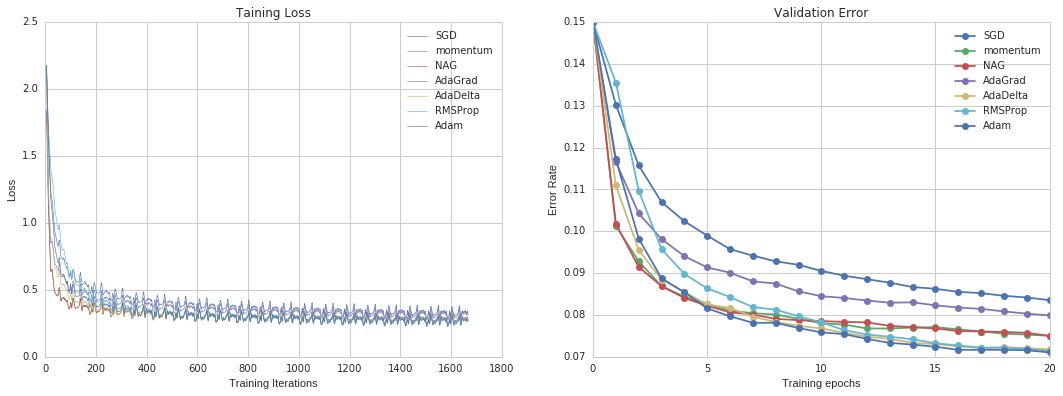
\includegraphics[width=450pt]{15}
	\centering
	\caption{Comparision of loss for models with different optimizers}
\end{figure}

\section{Regularization}
Regularization is a set of techniques used in machine learning, including deep learning, to prevent overfitting and improve the generalization performance of models. Overfitting occurs when a model learns to perform exceptionally well on the training data but struggles to generalize to new, unseen data. Regularization methods help prevent this by adding constraints to the learning process that encourage the model to produce simpler and more robust solutions.

We know that typically the loss function looks something like this

$$L(x,y) = \sum_{i=0}^n (y_i - f(x_i))^2$$

If our hypothesis looks like

$$f(x_i) = h_{\theta}x = \theta_0 + \theta_1 x^1 + \theta_2 x^2 + \theta_3 x^3 + \theta_4 x^4$$

When we penalize the weights $\theta_3$ and $\theta_4$ and make them too small, very close to zero. It makes those terms negligible and helps simplify the model.

$$f(x_i) = h_{\theta}x = \theta_0 + \theta_1 x^1 + \theta_2 x^2 + \cancel{\theta_3 x^3} + \cancel{\theta_4 x^4}$$
$$f(x_i) = h_{\theta}x = \theta_0 + \theta_1 x^1 + \theta_2 x^2$$

In deep learning, where neural networks can have millions of parameters, the risk of overfitting is significant. Regularization is crucial for the following reasons:
\begin{itemize}
\item \textbf{Preventing Overfitting}: Deep neural networks have the capacity to memorize the training data, which might lead to poor generalization. Regularization techniques impose constraints on the model's capacity, preventing it from fitting the noise in the training data and promoting better generalization to new data.

\item \textbf{Increasing Robustness}: Regularization encourages models to learn more robust features by preventing the network from becoming overly sensitive to small variations in the training data. This improves the model's ability to perform well on unseen examples.

\item \textbf{Enhancing Convergence}: In some cases, regularization can help the optimization process by smoothing the loss surface and reducing the risk of getting stuck in sharp, narrow valleys.
\end{itemize}

\textbf{Common Regularization Techniques}:

Several regularization techniques are used in deep learning:
\begin{enumerate}
\item \textbf{L2 Regularization (Weight Decay)}: This adds a penalty term to the loss function based on the magnitude of the weights. It discourages large weight values and promotes a more distributed representation of features.

\item \textbf{L1 Regularization}: Similar to L2 regularization, but it encourages sparsity in the weight values, effectively leading to some weights being exactly zero.

\item \textbf{Dropout}: This technique randomly drops a fraction of units (neurons) during each training iteration. It helps prevent co-adaptation of neurons and encourages the network to learn more diverse and robust features.

\item \textbf{Early Stopping}: Monitoring the model's performance on a validation set and stopping training once the performance starts to degrade can prevent overfitting.

\item \textbf{Data Augmentation}: Introducing variations to the training data by applying transformations like rotation, scaling, and cropping helps the model generalize better.

\item \textbf{Batch Normalization}: This technique normalizes the activations within each mini-batch, helping to stabilize and accelerate training.
\end{enumerate}

The choice of regularization technique depends on the problem, the architecture of the neural network, and the amount of available data. Experimentation and validation are necessary to determine the most effective regularization approach for a given task.

\subsection{L2 Regularization}
L2 regularization, also known as weight decay, ridge regression or Tikhonov regularization is a commonly used technique in machine learning and deep learning to prevent overfitting. It involves adding a penalty term to the loss function that discourages the model from having large weights. By doing so, L2 regularization promotes simpler models and reduces the risk of overfitting by preventing the model from fitting the noise in the training data.

L2 regularization adds a penalty term to the loss function based on the sum of squared weights. This technique promotes simpler models, helps prevent overfitting, and encourages better generalization to new data.

L2 regularization helps in the following ways:

\begin{enumerate}
\item \textbf{Preventing Overfitting}: By penalizing large weights, L2 regularization discourages the model from relying too much on individual features. This prevents the model from fitting the training data's noise and helps it generalize better to new, unseen data.

\item \textbf{Smoother Learning}: The regularization term encourages the model to distribute its learning across multiple features, leading to a smoother and more robust learning process.

\item \textbf{Regularizing High-Dimensional Models}: In deep learning, models often have a high number of parameters, which increases the risk of overfitting. L2 regularization provides a way to control the complexity of such models.
\end{enumerate}
\textbf{Mathematical Formulation}:

The L2 regularization term is added to the original loss function. Let's consider a simple linear regression case with squared error loss:

Original Loss: \( L(\theta) = \frac{1}{2n} \sum_{i=1}^{n} (y_i - f(x_i, \theta))^2 \)

L2 Regularization Term: \( \lambda \cdot \frac{1}{2} \sum_{j=1}^{p} \theta_j^2 \)

Here, \( \theta \) represents the model's parameters (weights), \( n \) is the number of data points, \( p \) is the number of features, \( y_i \) is the target value for the \( i \)-th data point, \( x_i \) is the input features for the \( i \)-th data point, \( f(x_i, \theta) \) is the predicted output, and \( \lambda \) is the regularization strength hyperparameter.

The combined loss function with L2 regularization becomes:
\[ L_\text{L2}(\theta) = L(\theta) + \lambda \cdot \frac{1}{2} \sum_{j=1}^{p} \theta_j^2 \]

The hyperparameter \( \lambda \) controls the strength of the regularization. Larger values of \( \lambda \) result in stronger regularization. The choice of \( \lambda \) depends on the specific problem and can be determined through cross-validation.


\subsection{L1 Regularization}

L1 regularization, also known as Lasso regularization, is a technique used in machine learning and deep learning to prevent overfitting by adding a penalty term to the loss function. L1 regularization encourages the model to have sparse weights, which means that it will set some of the weights to exactly zero. This promotes feature selection and simplification of the model.

L1 and L2 regularization have different effects on the model's weights. L1 encourages sparsity and feature selection, while L2 encourages small weight values. Depending on the problem, one regularization type may be more suitable than the other.

\textbf{How L1 Regularization Helps}:

L1 regularization helps in the following ways:
\begin{enumerate}
\item \textbf{Feature Selection}: L1 regularization encourages the model to set some of the weight parameters (\( \theta \)) to zero, effectively performing feature selection. This is valuable in cases where not all features contribute equally to the model's performance.

\item \textbf{Simplicity}: The sparsity induced by L1 regularization leads to a simpler model, which is often easier to interpret and generalizes well to new data.

\item \textbf{Reducing Overfitting}: By setting some weights to zero, L1 regularization simplifies the model's complexity and reduces the risk of overfitting, as it prevents the model from fitting noise in the training data.
\end{enumerate}

\textbf{Mathematical Formulation}:

Similar to L2 regularization, the L1 regularization term is added to the original loss function. Let's consider a simple linear regression case with squared error loss:

Original Loss: \( L(\theta) = \frac{1}{2n} \sum_{i=1}^{n} (y_i - f(x_i, \theta))^2 \)

L1 Regularization Term: \( \lambda \cdot \sum_{j=1}^{p} |\theta_j| \)

Here, the notation \( |\theta_j| \) represents the absolute value of the \( j \)-th weight parameter, and \( \lambda \) is the regularization strength hyperparameter.

The combined loss function with L1 regularization becomes:
\[ L_\text{L1}(\theta) = L(\theta) + \lambda \cdot \sum_{j=1}^{p} |\theta_j| \]


The hyperparameter \( \lambda \) controls the strength of the regularization. Larger values of \( \lambda \) result in stronger regularization. The choice of \( \lambda \) depends on the specific problem and can be determined through techniques like cross-validation.

\subsection{Noise Robustness}

Noise robustness is a regularization technique used in machine learning and deep learning to improve the generalization performance of models by introducing controlled amounts of noise to the input data during training. This technique is particularly effective in preventing models from overfitting to the specific details of the training data and helps the model learn more relevant and robust features.

The primary motivation behind noise robustness as a regularization technique is to make the model more resilient to variations and uncertainties present in real-world data. By exposing the model to noisy input, it learns to focus on the underlying patterns and relevant features while ignoring the noise and irrelevant details.

Noise can be introduced to the training data in various ways:
\begin{enumerate}
	\item \textbf{Input Noise}: Adding random noise to the input features before feeding them to the model. This is also called data augmentation.

	\item \textbf{Label Noise}: Introducing noise to the target labels, which helps the model learn to tolerate inaccuracies in the training labels.

	\item \textbf{Adding noise to weights}: Noise injection can be much more powerful than simply shrinking the parameters. Noise applied to hidden units is so important that it merits its own separate discussion. Generally adding noise to weights and performing a dropout is seen as a great regularization strategy. Adding noise to weights encourages stability.
\end{enumerate}


\textbf{Choosing Noise Levels}:

While noise robustness is beneficial, it's important to strike a balance. Introducing too much noise can hinder the learning process, and excessively noisy data might not effectively represent the underlying patterns.

The amount of noise introduced should be determined through experimentation and validation. Cross-validation and monitoring the model's performance on validation data can help identify the optimal noise levels.

\textbf{Adding Noise to Outputs}

Suppose we have a neural network with an activation function \( f \) applied to its outputs. Adding noise to the outputs can be represented as follows:

Original Output: \( y = f(x) \)

Noisy Output: \( \tilde{y} = f(x) + \epsilon \)

Here, \( \epsilon \) represents the added noise. This noise introduces small variations to the model's predictions during training. Mathematically, this can be seen as adding a regularization term to the loss function:

Regularized Loss: \( \mathcal{L}_\text{regularized} = \mathcal{L}(y, \tilde{y}) + \lambda R(\epsilon) \)

Where \( \mathcal{L}(y, \tilde{y}) \) is the original loss function, \( \lambda \) controls the strength of regularization, and \( R(\epsilon) \) quantifies the amount of noise introduced.

\begin{figure}[ht]
	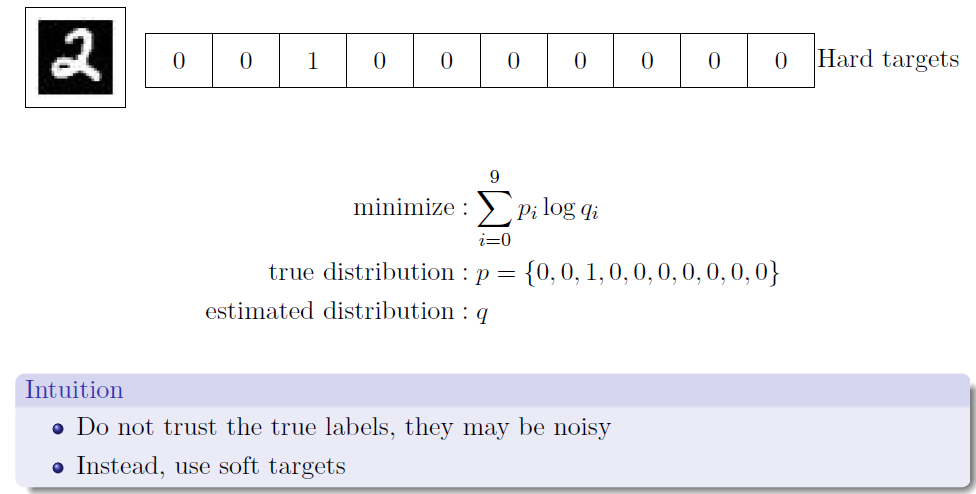
\includegraphics[width=450pt]{20}
	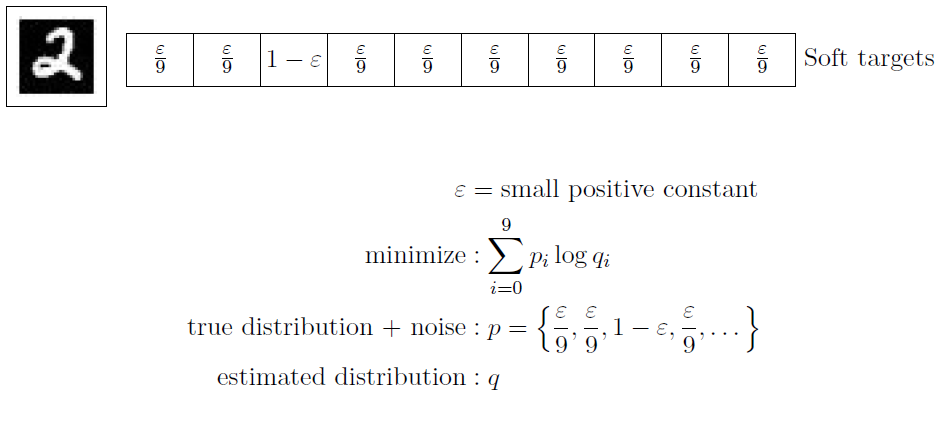
\includegraphics[width=450pt]{21}
	\centering
\end{figure}

\textbf{Adding Noise to Weights}:

Let $\epsilon \sim \mathcal{N}(0, \sigma^2)$ be the noise to be added to the weights.

$$\tilde{x_i} = x_i + \epsilon_i$$
$$\hat{y} = \sum_{i=1}^n x_i w_i$$
$$\tilde{y} = \sum_{i=1}^n\tilde{x_i} w_i$$
$$= \sum_{i=1}^n x_i w_i + \sum_{i=1}^n w_i \epsilon_i$$

Adding noise to the weights is another form of regularization. This can be represented as follows:

Original Weight Update: \( \Delta w = -\eta \cdot \nabla \mathcal{L} \)

Noisy Weight Update: \( \Delta \tilde{w} = -\eta \cdot (\nabla \mathcal{L} + \epsilon) \)

Here, \( \eta \) is the learning rate, \( \nabla \mathcal{L} \) is the gradient of the loss, and \( \epsilon \) represents the added noise. The noise affects the weight update direction and magnitude, introducing randomness.

\textbf{Regularization Effect}:

Adding noise to the outputs and weights introduces randomness into the training process, preventing the model from fitting the training data noise too closely. This randomness helps the model avoid overfitting, as it encourages the model to learn more robust features that generalize better to unseen data.

\textbf{Trade-offs and Considerations}:

The strength of noise added (\( \lambda \) in output noise and the magnitude of \( \epsilon \) in weight noise) should be carefully tuned. Too much noise can hinder learning, while too little may not provide sufficient regularization.

In summary, adding noise to the outputs and weights introduces controlled randomness into the training process, preventing overfitting and improving generalization. Mathematically, this can be seen as modifying the loss function and weight updates to include regularization terms related to the added noise.


\subsection{Ensemble Methods}

Ensemble methods are techniques in machine learning and deep learning that combine the predictions of multiple individual models to create a stronger, more robust final model. While the primary purpose of ensemble methods is to improve predictive performance, they also provide an effective way to achieve regularization and prevent overfitting.

Ensemble methods work by training multiple models independently and then combining their predictions to make a final decision. There are several types of ensemble methods, including bagging, boosting, and stacking.

\textbf{Regularization Effect of Ensemble Methods}:

Ensemble methods contribute to regularization through several mechanisms:

1. \textbf{Model Diversity}: Ensemble methods often involve training different models using different subsets of data or different features. This diversity among individual models prevents them from fitting the training data noise and overemphasizing specific patterns.

2. \textbf{Error Correction}: When combining the predictions of individual models, ensemble methods tend to reduce the impact of errors made by any one model. This error correction effect helps the ensemble make more robust and reliable predictions.

3. \textbf{Bias-Variance Trade-off}: Ensemble methods can balance the bias-variance trade-off. High-variance models (those prone to overfitting) are often combined with low-variance models (more robust but potentially biased), resulting in a better trade-off between underfitting and overfitting.

4. \textbf{Combining Weak Models}: Ensemble methods can effectively combine weak learners (models that perform only slightly better than random guessing) to create a strong learner. This strategy discourages the ensemble from fitting the noise in the data, thereby promoting regularization.

\textbf{Ensemble Techniques as Regularizers}:

1. \textbf{Bagging (Bootstrap Aggregating)}: Bagging creates an ensemble of models by training each model on a randomly sampled subset of the training data with replacement. It reduces overfitting by averaging out individual model errors.

2. \textbf{Boosting}: Boosting iteratively builds a strong model by giving more weight to misclassified instances. This adaptive boosting process effectively corrects model errors and contributes to regularization.

3. \textbf{Random Forests}: Random forests combine bagging with decision trees. Each tree is trained on a subset of features, reducing the risk of overfitting.

4. \textbf{Gradient Boosting}: Gradient boosting builds an ensemble by iteratively fitting models to the residuals of the previous models. This process corrects errors and helps the ensemble generalize better.

\textbf{Considerations}:

While ensemble methods provide regularization benefits, they may also introduce complexity and computational overhead. Care should be taken to choose appropriate ensemble techniques and tune their hyperparameters to achieve the desired level of regularization.

In summary, ensemble methods enhance model performance by combining multiple models' predictions. They also provide regularization by promoting model diversity, error correction, bias-variance trade-off, and combining weak models, which helps prevent overfitting and improves generalization.


\subsection{Dropout}
Deep neural networks contain multiple non-linear hidden layers and this makes them very expressive models that can learn very complicated relationships between their inputs and outputs. With limited training data, however, many of these complicated relationships will be the result of sampling noise, so they will exist in the training set but not in real test data even if it is drawn from the same distribution. Dropout is a technique that addresses these issues. It prevents overfitting and provides a way of approximately combining exponentially many different neural network architectures efficiently. By dropping a unit out, we mean temporarily removing it from the network, along with all its incoming and outgoing connections. 

In the simplest case, each unit is retained with a fixed probability p independent of other units, where p can be chosen using a validation set or can simply be set at 0.5, which seems to be close to optimal for a wide range of networks and tasks. 

\begin{figure}[ht]
	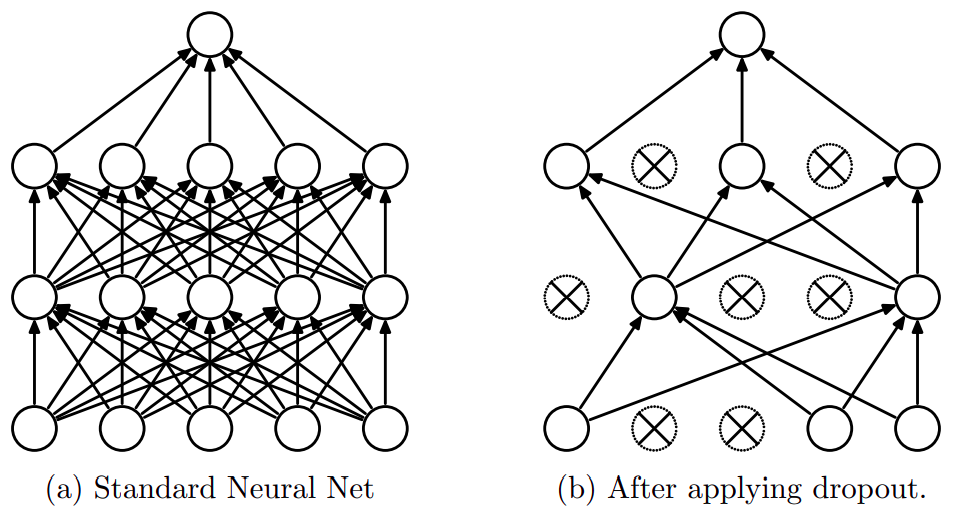
\includegraphics[width=250pt]{16}
	\centering 
	\caption{Dropout Neural Net Model. Left: A standard neural net with 2 hidden layers. Right: An example of a thinned net produced by applying dropout to the network on the left. Crossed units have been dropped.}
\end{figure}

Applying dropout to a neural network amounts to sampling a “thinned” network from it. The thinned network consists of all the units that survived dropout.

\begin{figure}[ht]
	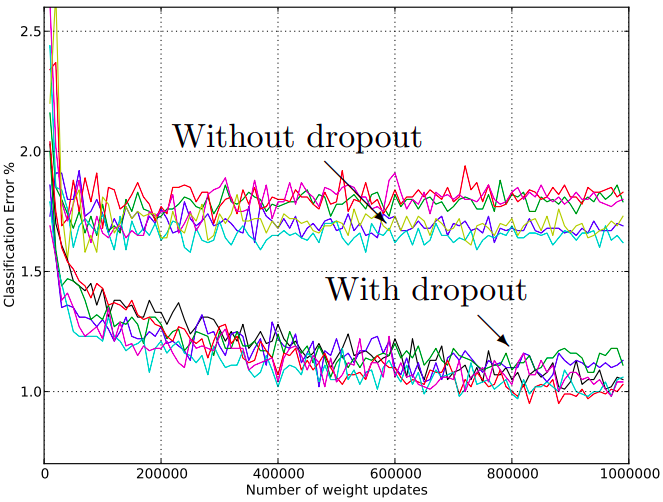
\includegraphics[width=250pt]{17}
	\centering
\end{figure}

\begin{figure}[ht]
	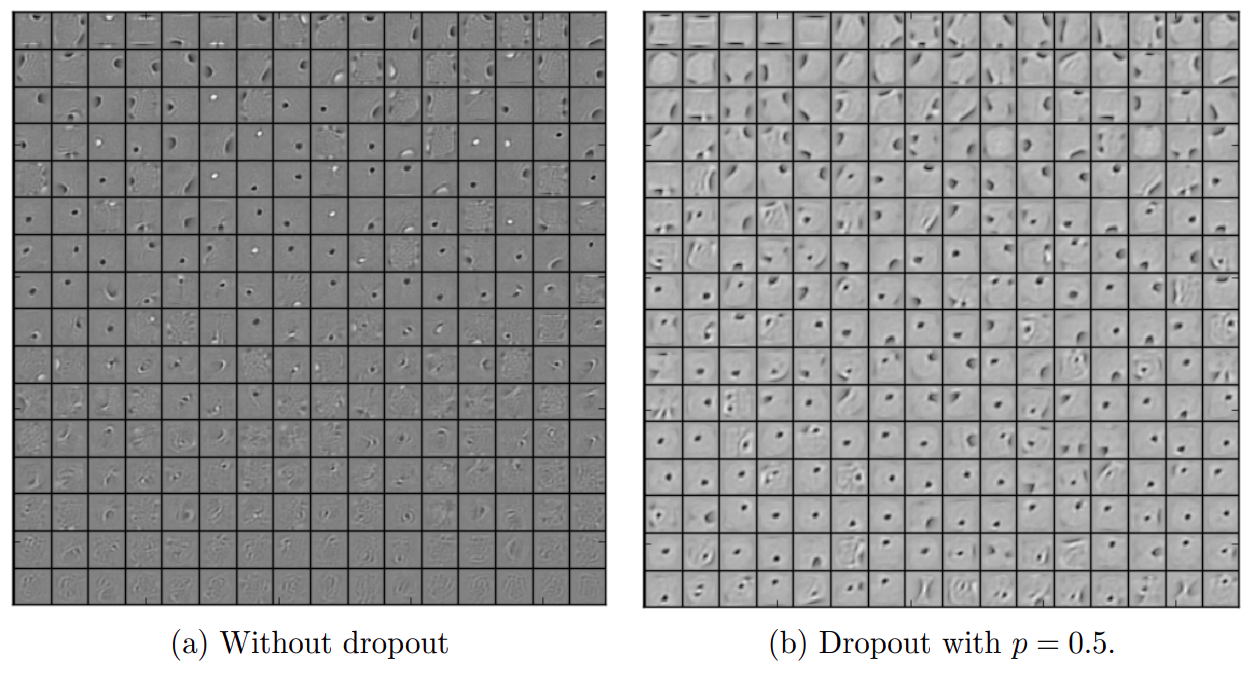
\includegraphics[width=450pt]{18}
	\centering 
	\caption{Features learned on MNIST by 256 hidden unit RBMs. The features are ordered by L2 norm.}
\end{figure}

In PyTorch, the dropout is added after every neural network layer with it's parameter p.

\begin{verbatim}
class Model(nn.Module):
    def __init__(self, n1, n2, dropout_p):
        super(CustomModel, self).__init__()
        
        self.dense_layers = nn.Sequential(
            nn.Linear(in_features=input_dim, out_features=n1),
            nn.Linear(in_features=n1, out_features=n2)
        )
        
        self.dropout = nn.Dropout(p=dropout_p)

    def forward(self, x):
        x = self.dense_layers(x)
        x = self.dropout(x)
        return x
\end{verbatim}


\clearpage
\subsection{Early Stopping}

Early stopping is a regularization technique used in machine learning and deep learning to prevent overfitting by monitoring a model's performance on a validation dataset during the training process. The idea behind early stopping is to halt the training process once the model's performance on the validation set starts to degrade, indicating that further training might lead to overfitting. Choosing the right patience parameter is crucial. Setting it too low might result in stopping prematurely, missing out on potential improvements. Setting it too high might allow overfitting to occur before stopping.

The process of early stopping involves the following steps:
\begin{enumerate}
	\item \textbf{Validation Set}: A separate validation dataset is set aside that the model does not use for training. This dataset is used to monitor the model's performance during training.

	\item  \textbf{Training and Monitoring}: The model is trained on the training dataset, and its performance is evaluated on the validation dataset at regular intervals (epochs). The performance metric, such as accuracy or loss, is recorded.

	\item  \textbf{Early Stopping Criterion}: A patience parameter is set, which determines how long the training process is allowed to continue without improvement on the validation performance. If the validation performance does not improve for a certain number of consecutive epochs (determined by patience), training is stopped.

	\item  \textbf{Model Selection}: The model's weights at the point of early stopping are used as the final model. These weights represent a point where the model's performance on unseen data (validation set) was at its best.
\end{enumerate}
\textbf{How Early Stopping Helps in Regularization}:

Early stopping serves as a form of regularization by preventing the model from being trained for too long, which can lead to overfitting. Here's how it helps:
\begin{itemize}
	\item \textbf{Avoiding Overfitting}: Early stopping prevents the model from continuing to learn from the noise and fluctuations present in the training data beyond a point where it's beneficial. This is especially important when the model's performance on the validation set starts to degrade, indicating overfitting tendencies.

	\item \textbf{Encouraging Simplicity}: By stopping training before the model fully adapts to the training data, early stopping encourages the model to remain simpler and prevents it from fitting the noise too closely.

	\item \textbf{Better Generalization}: The model's weights at the point of early stopping often generalize well to new, unseen data, as they capture the most relevant information without being overly influenced by noise.
\end{itemize}

The patience parameter is a key hyperparameter in the early stopping technique. It determines how many consecutive epochs the model's performance on the validation set can degrade before the training process is stopped. The patience parameter helps strike a balance between allowing the model to improve its performance and preventing overfitting.

\begin{figure}[ht]
	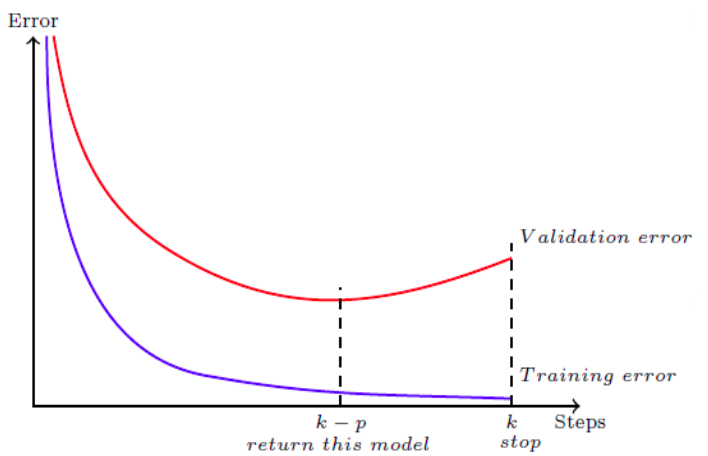
\includegraphics[width=250pt]{22}
	\centering
\end{figure}

\textbf{Mathematical Representation}:

Let's define the patience parameter as \( P \). During training, the model's performance on the validation set is monitored at the end of each epoch. If the validation performance does not improve for \( P \) consecutive epochs, the training process is stopped.

Mathematically, if \( \text{val\_loss}_i \) represents the validation loss at the \( i \)-th epoch, and \( \text{val\_loss}_{i-1} \) represents the validation loss at the \( (i-1) \)-th epoch, then the patience criterion can be written as:

\[ \text{if } \text{val\_loss}_i \geq \text{val\_loss}_{i-1} \text{ for } P \text{ consecutive epochs, stop training} \]

Here, \( P \) is the patience parameter that you set before starting training.

\textbf{How Patience Parameter Works}:

- If the validation performance improves from one epoch to the next, the patience counter is reset to zero.
- If the validation performance does not improve (or worsens) for consecutive epochs, the patience counter is incremented.
- Once the patience counter reaches the value of \( P \), the training process is stopped, assuming that the model's performance on the validation set is not improving.


\subsection{Data Augmentation}

Data augmentation is a technique used to artificially increase the diversity and size of a training dataset by applying various transformations to the existing data samples. These transformations create new instances of data that are similar to the original samples but have slight variations. Data augmentation is commonly used in deep learning to improve the generalization and performance of models.

The primary motivation behind data augmentation is to expose the model to a broader range of data variations, simulating real-world scenarios and enhancing the model's ability to generalize well to unseen data. This is especially valuable when the available training data is limited, as data augmentation effectively increases the effective size of the dataset.

Several common data augmentation techniques are used in deep learning:
\begin{enumerate}
	\item \textbf{Horizontal Flipping}: Flipping images horizontally, which is particularly useful for tasks like object recognition.

	\item \textbf{Random Cropping}: Cropping images to different sizes and positions to vary the perspective and focus of the model.

	\item \textbf{Rotation}: Rotating images by certain angles to account for orientation variations.

	\item \textbf{Zooming}: Zooming in or out on images to capture different levels of detail.

	\item \textbf{Brightness and Contrast Adjustments}: Changing the brightness and contrast of images to simulate different lighting conditions.

	\item \textbf{Color Jittering}: Slight changes in color values to simulate variations in lighting and environment.

	\item \textbf{Adding Noise}: Introducing random noise to images to simulate real-world imperfections.
\end{enumerate}

Data augmentation is applied during the training process. For each mini-batch of data, random transformations are applied to the samples before feeding them into the neural network. This introduces diversity and prevents the model from memorizing the training data.

While data augmentation is beneficial, care should be taken not to over-augment the data, which could lead to introducing unrealistic variations. Additionally, the choice of augmentation techniques should be based on the specific problem and domain.

\subsection{Batch Normalization}

Batch normalization (BatchNorm) is a technique used in deep neural networks to normalize the activations within each mini-batch during training. It helps stabilize and accelerate training by reducing internal covariate shifts, which is the phenomenon where the distribution of activations within layers changes during training.

Although BatchNorm provides regularization-like benefits, it is often used in conjunction with other regularization techniques such as L2 or dropout to enhance the model's regularizing effect further. Combining these techniques can lead to better generalization and prevent overfitting more effectively.

\section{Weight Initialization}
Weight initialization is an approach that has been proposed to reduce the vanishing gradient problem in deep networks.

It is suggested that the distribution of initial weights should vary according to activation function used and proposed to initialize the weights in networks with the logistic activation function using a Gaussian distribution with a zero mean and a standard deviation of $\frac{3.6}{\sqrt{n}}$, where $n$ is the number of neurons in a layer.

Recently, Yilmaz and Poli performed a theoretical analysis on how gradients are affected by the mean of the initial weights in deep neural networks using the logistic activation function and found that gradients do not vanish if the mean of the initial weights is set according to the formula: $max(-1,\frac{-8}{n})$. This simple strategy allows networks with 10 or 15 hidden layers to be trained very efficiently and effectively using the standard backpropagation.

\subsection{Weight Initialization for tanh and sigmoid Activation Functions}
The current standard approach for initialization of the weights of neural network layers and nodes that use the Sigmoid or TanH activation function is called “glorot” or “xavier” initialization.

\textbf{Xavier Weight Initialization}
The xavier initialization method is calculated as a random number with a uniform probability distribution $(U)$ between the range $\frac{-1}{\sqrt{n}}$ and $\frac{1}{\sqrt{n}}$, where n is the number of inputs to the node.

$$w_\text{initial} = U\lt[-\lt(\frac{1}{\sqrt{n}}\rt), \frac{1}{\sqrt{n}}\rt]$$

\textbf{Normalized Xavier Weight Initialization}
The normalized xavier initialization method is calculated as a random number with a uniform probability distribution $(U)$ between the range $-\frac{\sqrt{6}}{\sqrt{n + m}}$ and $\frac{\sqrt{6}}{\sqrt{n+m}}$, where $n$ is the number of inputs to the node (e.g. number of nodes in the previous layer) and $m$ is the number of outputs from the layer (e.g. number of nodes in the current layer).

\[ w_\text{initial} = U\left[ -\frac{\sqrt{6}}{\sqrt{n + m}}, \frac{\sqrt{6}}{\sqrt{n + m}} \right] \]

\subsection{Weight Initialization for ReLU Activation Function}

The “xavier” weight initialization was found to have problems when used to initialize networks that use the rectified linear (ReLU) activation function.

As such, a modified version of the approach was developed specifically for nodes and layers that use ReLU activation, popular in the hidden layers of most multilayer Perceptron and convolutional neural network models.

\textbf{He et al. initialization/ MSRA Initialization}
The he initialization method is calculated as a random number with a Gaussian probability distribution $(G)$ with a mean of 0.0 and a standard deviation of $\sqrt{\frac{2}{n}}$, where $n$ is the number of inputs to the node.

We typically use this method when we are training very deep neural networks that use a ReLU-like activation function (in particular, a “PReLU,” or Parametric Rectified Linear Unit).

$$w_\text{initial} = G\lt(0.0, \sqrt{\frac{2}{n}}\rt)$$

\chapter{Convolutional Neural Networks}

\section{Previous Developments in Computer Vision}
\subsection{1959: The first digital scanner was invented}
The invention of the first digital image scanner in 1959 marked a pivotal moment in the evolution of computer vision and paved the way for groundbreaking advancements in image processing and analysis. Prior to this breakthrough, computers were incapable of understanding and manipulating visual information, a significant limitation in their ability to interact with the real world.

The concept of converting images into numerical representations, known as digitization, revolutionized the way computers could perceive and process visual data. By breaking down images into grids of tiny squares, called pixels, and assigning each pixel a numerical value based on its brightness or color, computers could now store, transmit, and manipulate images in a digital format.

This groundbreaking innovation, developed by Russell Kirsch and his team at the National Bureau of Standards, transformed the field of computer vision, laying the foundation for a wide range of applications that continue to shape our world today. From medical imaging to satellite imagery, facial recognition to self-driving cars, digital image processing has become an indispensable tool in modern society.

\subsection{1963: Larry Roberts, the father of Computer Vision}
In his groundbreaking 1963 paper, "Machine Perception of Three-Dimensional Solids," Larry Roberts, often regarded as the "father of computer vision," laid the groundwork for extracting 3D information from 2D photographs, a fundamental challenge in the field of computer vision. Roberts' work paved the way for numerous advancements in 3D reconstruction, object recognition, and scene understanding.

Roberts' approach involved analyzing multiple images of an object taken from different viewpoints. By identifying corresponding points in each image and applying geometric principles, he could infer the object's 3D structure. This technique, known as structure from motion, has become a cornerstone of computer vision and has found applications in robotics, augmented reality, and medical imaging.

\subsection{1966: Marvin Minsky}

In 1966, Marvin Minsky, a pioneer in the field of artificial intelligence, famously challenged a graduate student with a seemingly straightforward task: connect a camera to a computer and program it to describe what it sees. While the assignment sounded simple, it encapsulated the profound complexity of replicating human vision in machines.

This seemingly simple task turned out to be a daunting undertaking, highlighting the intricate nature of human visual perception. Humans effortlessly interpret the visual world, recognizing objects, understanding scenes, and inferring depth and motion. However, translating this ability into machine code proved to be a far more challenging task.

Minsky's challenge resonated within the AI community, sparking a surge of research into computer vision. Scientists began to explore various approaches to enable computers to perceive and understand visual information. This led to the development of techniques like image segmentation, object recognition, and scene understanding, which have revolutionized fields such as robotics, self-driving cars, and medical imaging.

\subsection{1980: Neocognition}
In 1980, a Japanese computer scientist named Kunihiko Fukushima made a groundbreaking contribution to the field of artificial intelligence by developing the "neocognitron," a neural network architecture that laid the foundation for modern convolutional neural networks (CNNs). CNNs have revolutionized computer vision, enabling machines to achieve remarkable feats in image and object recognition, surpassing human performance in many tasks.

Fukushima's neocognitron was inspired by the physiological structure of the human visual system, particularly the organization of neurons in the visual cortex. He proposed a hierarchical architecture composed of layers of simple cells (S-cells) and complex cells (C-cells), mimicking the receptive fields of neurons in the visual system.

S-cells extract local features from the input image, while C-cells combine these features to detect more complex patterns. This hierarchical organization allows the neocognitron to learn and recognize increasingly complex patterns as the input signal progresses through the layers.

\begin{figure}[ht]
	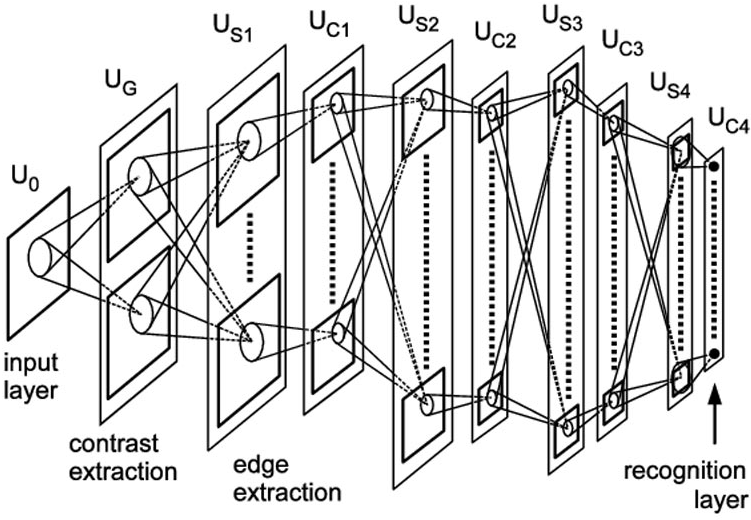
\includegraphics[width=250pt]{46}
	\centering
	\caption{Architecture of Neocognition}
\end{figure}
Fukushima's neocognitron demonstrated the potential of hierarchical neural networks for image recognition tasks, paving the way for the development of modern CNNs. While the neocognitron itself was limited in its capabilities due to computational constraints, it laid the conceptual groundwork for the powerful CNNs that we use today.

The impact of Fukushima's work is evident in the widespread adoption of CNNs in various fields, including computer vision, robotics, medical imaging, and autonomous vehicles. CNNs have enabled machines to perform tasks such as face recognition, medical image analysis, and self-driving navigation with remarkable accuracy.

Fukushima's neocognitron stands as a landmark achievement in the history of artificial intelligence, marking a pivotal moment in the development of computer vision and machine learning. His work continues to inspire researchers and shape the future of AI, as we strive to create machines that can perceive and understand the world around us with ever-increasing sophistication.

\subsection{2001: Viola-Jones Face Detection}
In 2001, Paul Viola and Michael Jones used a cascade of boosted decision trees to implement a fast and robust face detector suitable for use in handheld digital cameras. Their classifier localizes a face using essentially a sliding window approach in which many windows are examined and rejected if they do not contain faces. 

Viola and Jones had the insight that faces had certain patterns of light and dark patches that they could exploit. There is a difference in light intensity between the eye region and the upper cheeks. There is also a difference in light intensity between the nose bridge and the two eyes on either side.

The Viola-Jones framework had a profound impact on computer vision and its applications. It became the standard approach for face detection, enabling advancements in various fields, including:

\begin{figure}[ht]
	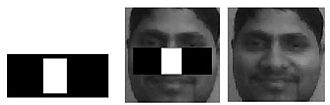
\includegraphics[width=150pt]{24}
	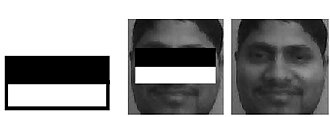
\includegraphics[width=150pt]{25}
	\centering
\end{figure}

\begin{enumerate}
\item Facial recognition: Viola-Jones paved the way for modern facial recognition systems, with applications in security, social media, and user authentication.

\item Surveillance systems: The framework enabled real-time face detection in surveillance footage, enhancing security and monitoring capabilities.

\item Human-computer interaction: Viola-Jones facilitated the development of human-computer interfaces that could recognize and respond to facial expressions and gestures.
\end{enumerate}

\section{Limitations of Vanilla Deep Neural Networks}

The fundamental goal in applying deep learning to computer vision is to revolutionize the way we process and understand data. One of the most significant advancements deep learning offers is the ability to remove the cumbersome and ultimately limiting process of feature selection. In traditional computer vision approaches, feature selection involves manually defining and extracting relevant characteristics or patterns from images. This process can be highly labor-intensive, requiring domain expertise, and is often inadequate for handling the complexity and diversity of real-world visual data.


One crucial component of deep learning models is the architecture of the neural network. In the provided example using the MNIST dataset, images are relatively small at 28 x 28 pixels and are in black and white. In such cases, a fully connected layer, where each neuron connects to every pixel in the input image, is manageable. However, this technique does not scale well as images grow larger or more complex.

For instance, consider a full-color image of 200 x 200 pixels. In this scenario, the input layer of a fully connected neural network would require 200 x 200 x 3 = 120,000 weights (assuming three color channels: red, green, and blue). Each weight corresponds to a connection between a neuron in the hidden layer and a pixel in the image. As images increase in size and complexity, the number of weights grows exponentially. This leads to several challenges:

\begin{enumerate}
	\item \textbf{Computational Complexity}: Managing such a large number of parameters becomes computationally intensive and may require substantial processing power, making training and inference slower and more resource-intensive.

	\item \textbf{Overfitting}: A high number of parameters increases the risk of overfitting, where the model fits the training data too closely and performs poorly on unseen data.

	\item \textbf{Lack of Spatial Awareness}: Fully connected layers do not inherently capture the spatial relationships and hierarchical features present in images, which are vital for accurate computer vision tasks.
\end{enumerate}

\section{The Role of Convolutional Neural Networks (CNNs)}

Deep learning, particularly Convolutional Neural Networks (CNNs), has transformed this paradigm. Instead of relying on handcrafted features, deep learning models can automatically learn relevant features directly from raw image data. This remarkable capability allows computer vision systems to adapt to various tasks without the need for explicit feature engineering. Deep learning models excel in capturing hierarchical features, from edges to textures to object parts, which makes them highly effective in image understanding.

Convolutional Neural Networks (CNNs) have emerged as the architecture of choice for image-related tasks. CNNs are designed to efficiently capture spatial hierarchies, share parameters across the image, and reduce the number of weights through convolutional layers. They excel in managing larger and more complex images, making them a cornerstone of modern computer vision systems. CNNs have revolutionized the field by allowing deep learning models to scale gracefully and effectively handle the complexities of real-world visual data.


\section{The Convolution Operation}
Mathematically the convolutional operation can be denoted as follows:
$$s(t) = \int{x(a) \cdot w(t-a)da}$$
In machine learning the convolution opertaion will be typically denoted by an asterisk $(\ast)$.
$$s(t) = (x \ast w)(t)$$
$\textrm{where:}\\ x = \textrm{inputs} \\ w = \textrm{kernel} \\ s = \textrm{feature map or the output of the convolution}$

In convolutional neural network terminology, the first argument to convolution is often referred
 to as the input, and the second argumant as the kernel. The output of this operation is referred to as the feater map. In realistic applications of deep learning CNNs where we are dealing with matrix of pixels, this operation is discretized and the mathematical operation can then be defined as:

$$s(t) = \sum_{a=-\infty}^{\infty}x(a)\cdot w(t-a)$$

\begin{figure}[ht]
	
\includegraphics[width=100pt]{26}
	\centering
	\caption{An animation of a 2D convolution operation}
\end{figure}

In machine learning applications, the input is usually a multidimensional array of data and the kernel is usually a multidimensional array of parameters that are adapted by the learning algorithm. We will refer to these multidimensional arrays as tensors. Because each element of the input and kernel must be explicitly stored separately, we usually assume that these functions are zero everywhere but the finite set of points for which we store the values. This means that in practice we can implement the infinite summation as a summation over a finite number of array elements.

Finally, we often use convolutions over more than one axis at a time. For example, if we use a two-dimensional image I as our input, we probably also want to use a two-dimensional kernel K:

$$S(i,j) = (I \ast K)(i, j) = \sum_m \sum_n I(m,n)K(i-m, j-n)$$

Convolution is commutative, meaning we can equivalently write:
$$S(i,j) = (I \ast K)(i, j) = \sum_m \sum_n I(i-m,j-n)K(m, n)$$

Many neural network libraries implement a related function called the cross-correlation, which is the same as convolution but without flipping the kernel. Some neural network libraries implement cross-correlation but call it the convolution operation.
$$S(i,j) = (I \ast K)(i, j) = \sum_m \sum_n I(i+m,j+n)K(m, n)$$

\begin{figure}[ht]
	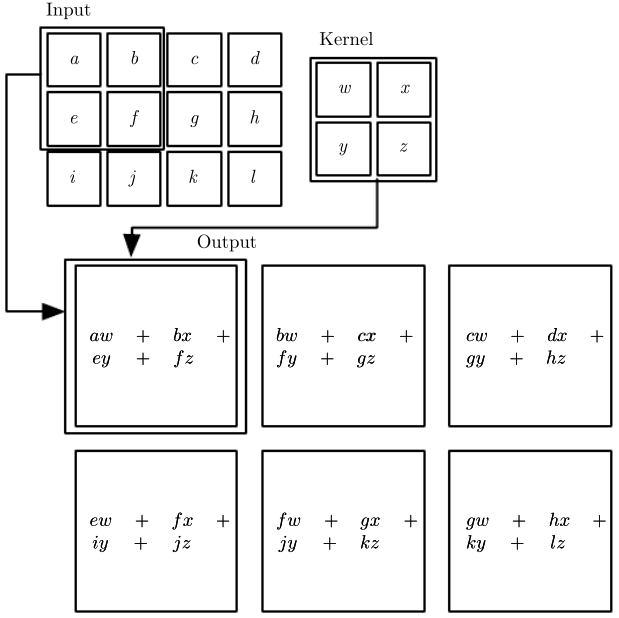
\includegraphics[width=250pt]{27}
	\centering
	\caption{An example of 2-D convolution without kernel-flipping. In this case we restrict the output to only positions where the kernel lies entirely within the image, called “valid” convolution in some contexts. We draw boxes with arrows to indicate how the upper-left element of the output tensor is formed by applying the kernel to the corresponding upper-left region of the input tensor.}
\end{figure}

Convolution leverages three important ideas that can help improve a machine learning system: 
\begin{enumerate}
	\item Sparse interactions
	\item Parameter sharing
	\item Equivariant representations.
\end{enumerate}

\subsection{Sparse Interactions}

\begin{figure}[ht]
	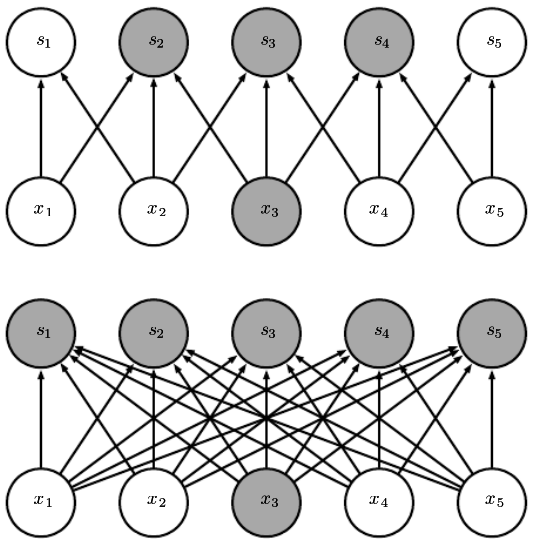
\includegraphics[width=250pt]{28}
	\centering
	\caption{Sparse connectivity, viewed from below: We highlight one input unit, $x_3$ , and also highlight the output units in $s$ that are affected by this unit. (Top) When $s$ is formed by convolution with a kernel of width 3, only three outputs are affected by $x$. (Bottom) When $s$ is formed by matrix multiplication, connectivity is no longer sparse, so all of the outputs are affected by $x_3$.}
\end{figure}

\begin{figure}[ht]
	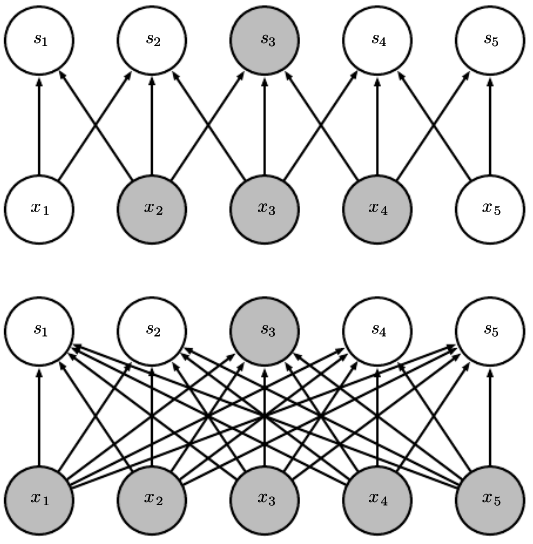
\includegraphics[width=250pt]{29}
	\centering
	\caption{Sparse connectivity, viewed from above: We highlight one output unit, $s_3$ , and also highlight the input units in $x$ that affect this unit. These units are known as the receptive field of $s_3$. (Top) When $s$ is formed by convolution with a kernel of width 3, only three inputs affect $s_3$. (Bottom) When $s$ is formed by matrix multiplication, connectivity is no longer sparse, so all of the inputs affect $s_3$.}
\end{figure}

\begin{figure}[ht]
	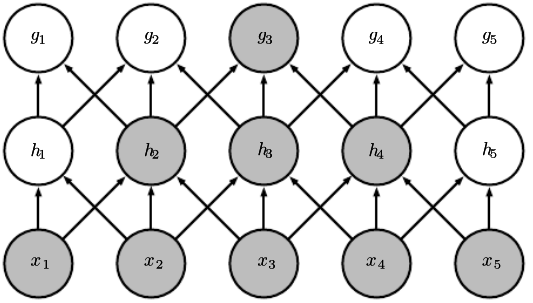
\includegraphics[width=250pt]{30}
	\centering
	\caption{The receptive field of the units in the deeper layers of a convolutional network is larger than the receptive field of the units in the shallow layers. This effect increases if the network includes architectural features like strided convolution or pooling. This means that even though direct connections in a convolutional net are very sparse, units in the deeper layers can be indirectly connected to all or most of the input image.}
\end{figure}

Traditional neural network layers use matrix multiplication by a matrix of parameters with a separate parameter describing the interaction between each input unit and each output unit. This means every output unit interacts with every input unit. Convolutional networks, however, typically have sparse interactions (also referred to as \textbf{sparse connectivity} or \textbf{sparse weights}). This is accomplished by making the kernel smaller than the input. For example, when processing an image, the input image might have thousands or millions of pixels, but we can detect small, meaningful features such as edges with kernels that occupy only tens or hundreds of pixels. This means that we need to store fewer parameters, which both reduces the memory requirements of the model and improves its statistical efficiency. It also means that computing the output requires fewer operations. These improvements in efficiency are usually quite large.

If there are $m$ inputs and $n$ outputs, then matrix multiplication requires $m \times n$ parameters and the algorithms used in practice have $O(m \times n )$ runtime (per example). If we limit the number of connections each output may have to $k$, then the sparsely connected approach requires only $k \times n$ parameters and $O(k \times n)$ runtime.

Here are ways in which Sparse Interactions benefits over a typical DNN:
\begin{itemize}
\item Parameter Efficiency:
CNNs exploit sparse connectivity, meaning that each neuron is only connected to a local region of the input. This leads to a significant reduction in the number of parameters compared to DNNs, where each neuron is connected to every neuron in the previous layer. Fewer parameters make the model more memory-efficient and computationally faster, facilitating training and inference.

\item Translation Invariance:
The use of convolutional layers with sparse interactions promotes translation invariance. This means that a pattern (e.g., a feature or an object) can be detected regardless of its exact position in the input. This is particularly valuable for image processing tasks, where the location of an object within an image should not affect the network's ability to recognize it.

\item Hierarchical Feature Learning:
Sparse interactions allow CNNs to learn hierarchical features in a more effective way. Lower layers capture simple features like edges and textures, while higher layers capture more complex and abstract features. This hierarchical representation is crucial for recognizing and understanding the hierarchical structure in data, especially in images.

\item Local Receptive Fields:
CNNs use local receptive fields, meaning that each neuron is sensitive to a small region of the input. This local connectivity helps capture local patterns and ensures that nearby pixels or features are more strongly connected. DNNs lack this explicit local connectivity, and as a result, they may struggle to efficiently capture spatial relationships in structured data.

\item Memory and Computational Efficiency:
The sparse connectivity pattern reduces the computational and memory requirements during both training and inference. This efficiency is especially beneficial when dealing with large-scale datasets, high-resolution images, or resource-constrained environments.

\item Generalization to Various Input Sizes:
CNNs can handle inputs of varying sizes more effectively than fully connected networks. This is because the filters in convolutional layers are applied locally and can adapt to different spatial dimensions. In contrast, fully connected layers have a fixed number of parameters, making them less flexible when dealing with inputs of different sizes.

\item Better Handling of Spatially Structured Data:
CNNs are designed to handle spatially structured data, making them well-suited for tasks like image recognition, object detection, and segmentation. The sparse interactions and local connectivity in CNNs enable them to capture spatial hierarchies and patterns that may be challenging for fully connected networks to learn.
\end{itemize}

\subsection{Parameter Sharing}
\textbf{Parameter sharing} refers to using the same parameter for more than one function in a model. In a traditional neural net, each element of the weight matrix is used exactly once when computing the output of a layer. It is multiplied by one element of the input and then never revisited. As a synonym for parameter sharing, one can say that a network has tied weights, because the value of the weight applied to one input is tied to the value of a weight applied elsewhere. The parameter sharing used by the convolution operation means that rather than learning a separate set of parameters for every location, we learn only one set. This does not affect the runtime of forward propagation—it is still $O(k \times n)$—but it does further reduce the storage requirements of the model to $k$ parameters.

Parameter sharing in CNNs helps reduce the number of learnable parameters, making the network more efficient and capable of learning spatial hierarchies of features. This design is inspired by the local connectivity and weight sharing observed in the visual cortex of animals, making CNNs well-suited for tasks involving spatially structured data like images.

Here's how parameter sharing works:
\begin{itemize}
	\item Convolutional Layers: Instead of fully connecting each neuron to all neurons in the next layer, CNNs use convolutional layers. These layers apply convolution operations to the input data using learnable filters or kernels.

	\item Filters/Kernels: Filters are small, spatially local, and repeatedly applied across the entire input. Each filter is responsible for detecting a specific feature, such as edges, textures, or patterns, in the input data. The values of the filter's parameters are shared across the entire input.

	\item Parameter Sharing: In a convolutional layer, the same filter (set of parameters) is used at different spatial locations across the input. The key idea is that the filter's weights are shared, meaning the filter is slid or convolved across the input, computing the dot product at each position.

	\item For example, if a filter is detecting vertical edges, it will learn to do so at various positions in the input image. Instead of learning separate parameters for each position, the same set of parameters is reused, reducing the number of overall parameters in the network.

	\item Translation Invariance: Parameter sharing allows the network to learn features that are translationally invariant, meaning the network can recognize the same pattern regardless of its position in the input. This is particularly useful for tasks such as image recognition, where the position of an object in an image should not affect the network's ability to identify it.
\end{itemize}

\subsection{Equivariant Representations}
In the case of convolution, the particular form of parameter sharing causes the layer to have a property called \textbf{equivariance to translation}. To say a function is equivariant means that if the input changes, the output changes in the same way. Specifically, a function $f(x)$ is equivariant to a function $g$ if $f(g(x)) = g(f (x))$. In the case of convolution, if we let $g$ be any function that translates the input, i.e., shifts it, then the convolution function is equivariant to $g$. For example, let $I$ be a function giving image brightness at integer coordinates. Let $g$ be a function mapping one image function to another image function, such that $I' = g(I)$ is the image function with $I' (x, y) = I(x - 1, y)$. This shifts every pixel of $I$ one unit to the right. If we apply this transformation to $I$, then apply convolution, the result will be the same as if we applied convolution to $I'$ , then applied the transformation $g$ to the output.

In some cases, we may not wish to share parameters across the entire image. For example, if we are processing images that are cropped to be centered on an individual’s face, we probably want to extract different features at different locations—the part of the network processing the top of the face needs to look for eyebrows, while the part of the network processing the bottom of the face needs to look for a chin.

Convolution is not naturally equivariant to some other transformations, such as changes in the scale or rotation of an image. Other mechanisms are necessary for handling these kinds of transformations.

\section{Pooling}
A typical layer of a convolutional network consists of three stages: 
\begin{enumerate}
	\item In the first stage, the layer performs several convolutions in parallel to produce a set of linear activations. 
	\item In the second stage, each linear activation is run through a nonlinear activation function, such as the rectified linear activation function. This stage is sometimes called the detector stage. 
	\item In the third stage, we use a pooling function to modify the output of the layer further.
	\end{enumerate}

	\begin{figure}[ht]
	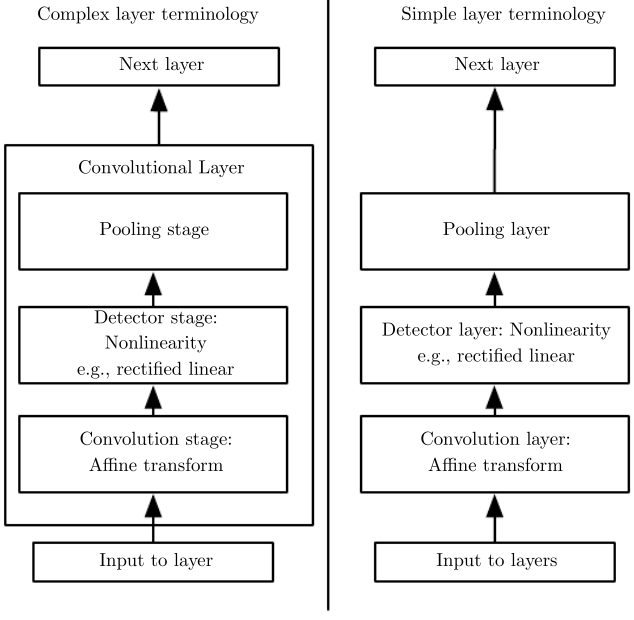
\includegraphics[width=250pt]{31}
	\centering
\end{figure}

A pooling function replaces the output of the net at a certain location with a summary statistic of the nearby outputs. For example, MaxPooling operation reports the maximum output within a rectangular neighborhood. Other p opular p o oling functions include the average of a rectangular neighborhood, the L2 norm of a rectangular neighborho od, or a weighted average based on the distance from the central pixel.

In all cases, pooling helps to make the representation become approximately invariant to small translations of the input. \textbf{Invariance to translation} means that if we translate the input by a small amount, the values of most of the pooled outputs do not change. Invariance to local translation can be a very useful property if we care more about whether some feature is present than exactly where it is. For example, when determining whether an image contains a face, we need not know the location of the eyes with pixel-perfect accuracy, we just need to know that there is an eye on the left side of the face and an eye on the right side of the face.

The use of pooling can be viewed as adding an infinitely strong prior that the function the layer learns must be invariant to small translations. When this assumption is correct, it can greatly improve the statistical efficiency of the network. Pooling over spatial regions produces invariance to translation, but if we pool over the outputs of separately parametrized convolutions, the features can learn which transformations to become invariant to.

Because pooling summarizes the responses over a whole neighborhood, it is possible to use fewer pooling units than detector units, by reporting summary statistics for pooling regions spaced k pixels apart rather than 1 pixel apart. This improves the computational efficiency of the network b ecause the next layer has roughly k times fewer inputs to pro cess. When the numb er of parameters in the next layer is a function of its input size (such as when the next layer is fully connected and based on matrix multiplication) this reduction in the input size can also result in improved statistical efficiency and reduced memory requirements for storing the parameters.

For many tasks, pooling is essential for handling inputs of varying size. For example, if we want to classify images of variable size, the input to the classification layer must have a fixed size. This is usually accomplished by varying the size of an offset between p ooling regions so that the classification layer always receives the same number of summary statistics regardless of the input size. For example, the final pooling layer of the network may be defined to output four sets of summary statistics, one for each quadrant of an image, regardless of the image size.

\begin{figure}[ht]
	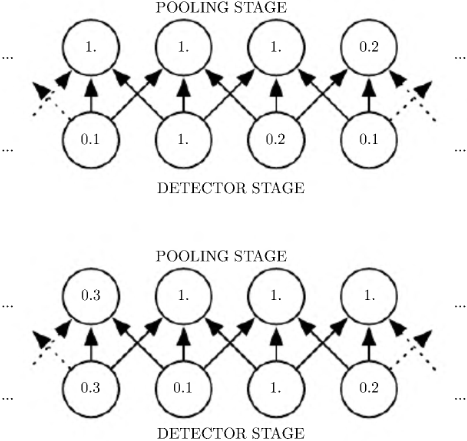
\includegraphics[width=250pt]{47}
	\centering
	\caption{Max p ooling introduces invariance. (Top) A view of the middle of the output of a convolutional layer. The b ottom row shows outputs of the nonlinearity. The top row shows the outputs of max po oling, with a stride of one pixel b etween p o oling regions and a p ooling region width of three pixels. A view of the same network, after (Bottom) the input has b een shifted to the right by one pixel. Every value in the b ottom row has changed, but only half of the values in the top row have changed, b ecause the max p ooling units are only sensitive to the maximum value in the neighborho od, not its exact location.}
\end{figure}

\begin{figure}[ht]
	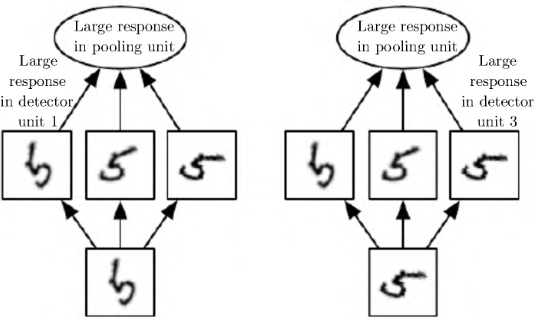
\includegraphics[width=250pt]{48}
	\centering
	\caption{Example of learned invariances: A pooling unit that pools over multiple features that are learned with separate parameters can learn to be invariant to transformations of the input. Here we show how a set of three learned filters and a max p ooling unit can learn to become invariant to rotation. All three filters are intended to detect a hand-written 5. Each filter attempts to match a slightly different orientation of the 5. When a 5 app ears in the input, the corresponding filter will match it and cause a large activation in a detector unit.}
\end{figure}

\section{Transfer Learning}
Transfer learning is a machine learning technique where a model developed for a particular task is reused as the starting point for a model on a second task. In the context of Convolutional Neural Networks (CNNs), transfer learning involves using a pre-trained model, often trained on a large dataset for a related task, as the starting point for a new task.

Transfer learning has been successfully applied to various computer vision tasks, such as image classification, object detection, and image segmentation. Popular pre-trained models for transfer learning include architectures like VGG16, ResNet, and Inception, which have been trained on large-scale image datasets like ImageNet. Researchers and practitioners often use these pre-trained models as a starting point for their specific computer vision applications.

Transfer learning in CNNs is particularly effective for several reasons:

\begin{itemize}
	\item Feature Reuse: The early layers of a CNN learn generic features that are applicable to a wide range of visual tasks. By reusing these features, the model can leverage the knowledge gained from the original task.

\item Data Efficiency: Transfer learning is especially beneficial when the new task has limited data. Instead of training a model from scratch, transfer learning allows the model to start with knowledge gained from a larger dataset, often resulting in better performance with less labeled data.

\item Computational Efficiency: Training deep neural networks from scratch on large datasets can be computationally expensive. Transfer learning reduces the computational cost by starting with a pre-trained model and fine-tuning it on the new task.
\end{itemize}

The intuition behind transfer learning lies in the idea that knowledge gained from solving one task can be beneficial for solving a different, but related task. In the context of neural networks, and specifically Convolutional Neural Networks (CNNs), the lower-level features learned by a model on a large dataset for a particular task (source task) can be useful as a starting point for a different but related task (target task).

Here's an intuitive breakdown of the key concepts:

\begin{itemize}
\item Learning Generic Features:
In the early layers of a deep neural network, especially in CNNs, the model tends to learn features that are generic and broadly applicable across different tasks. For example, in an image classification task, the early layers might learn to detect simple features like edges, textures, and basic shapes.

\item Task-Specific Learning:
As the neural network progresses through its layers, it refines its features to become more task-specific. The deeper layers capture complex and high-level representations that are crucial for the success of the original task.

\item Transferability of Features:
The intuition behind transfer learning is that these generic features learned in the early layers are transferable and can be applied to other tasks. For instance, if a CNN is trained on a large dataset for image classification, the low-level features it learned (like recognizing edges and textures) can be valuable for tasks such as object detection or segmentation.

\item Data Efficiency:
Transfer learning is particularly useful when the target task has limited labeled data. Instead of starting from scratch and training a model with insufficient data, one can leverage the knowledge encoded in the pre-trained model. This is especially crucial in scenarios where collecting labeled data for a new task is expensive or time-consuming.

\item Fine-Tuning for Adaptation:
To make the transferred features more suitable for the target task, fine-tuning is performed. During fine-tuning, the pre-trained model is adjusted on the target task's dataset. This allows the model to adapt its learned features to the specific nuances of the new task while retaining the valuable knowledge from the source task.

\item Computational Efficiency:
Training deep neural networks from scratch on large datasets can be computationally expensive. Transfer learning provides a way to leverage the pre-trained model's weights, reducing the computational cost. Fine-tuning is often faster and requires less computational resources than training a model entirely from the ground up.
\end{itemize}

Following are some ImageNet success stories which have contributed to models that are commonly used for transfer learning.

\subsection{AlexNet}
AlexNet, developed by researchers Alex Krizhevsky, Ilya Sutskever, and Geoffrey Hinton, stands as a landmark in the evolution of deep neural networks, particularly within the realm of computer vision. Its debut in 2012 initiated a resurgence of interest in the capabilities of deep learning for image recognition tasks, overcoming challenges such as vanishing gradients and computational limitations that had hindered the training of deep neural networks.

The model's triumph in the ImageNet Large-Scale Visual Recognition Challenge (ILSVRC) of 2012, where it outperformed competitors by a substantial margin, underscored the prowess of deep neural networks in image classification. This competition is renowned for its emphasis on challenging tasks involving a vast dataset containing a thousand distinct object classes.

A notable departure from its predecessors, AlexNet boasted an augmented network depth, comprising eight layers—five convolutional layers followed by three fully connected layers. This increased depth empowered the network to capture intricate hierarchical features within input data, thereby contributing to its superior performance.

The augmentation in network depth naturally led to a notable increase in the number of tunable parameters, enhancing the model's capacity to learn intricate and discriminative features. To address concerns of overfitting, AlexNet integrated regularization techniques, with dropout as a prominent example. This method involved randomly deactivating a fraction of neurons during training, thereby preventing reliance on specific neurons and fostering model robustness. Furthermore, the integration of data augmentation techniques artificially expanded the training dataset, introducing variations in input data to enhance the model's adaptability to diverse scenarios.

The temporal aspect of training AlexNet on the complete ImageNet dataset is a noteworthy consideration, requiring approximately six days to process the extensive dataset comprising 1.2 million images across a thousand object classes. This underscored the computational demands inherent in training deep neural networks on vast image datasets, emphasizing the importance of robust computational resources in advancing the field of deep learning.

\begin{figure}[ht]
	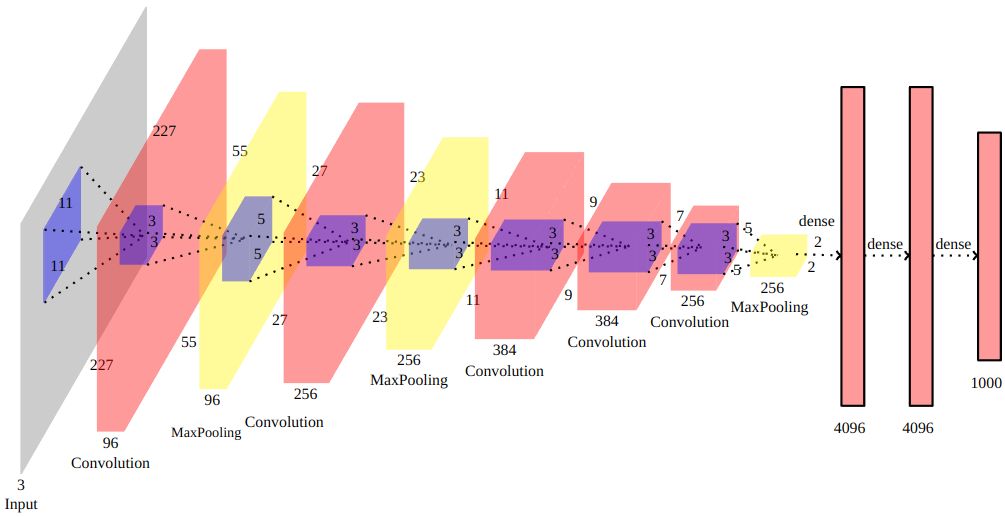
\includegraphics[width=350pt]{49}
	\centering
	\caption{Architecture of AlexNet}
\end{figure}

\subsection{ZFNet}
During the ImageNet Large Scale Visual Recognition Challenge (ILSVRC) in 2013, ZFNet garnered attention for its substantial advancements, surpassing the achievements of its predecessor, AlexNet.

A pivotal disparity between the two approaches lies in the selection of filter sizes. ZFNet opted for 7x7-sized filters, a departure from AlexNet's use of larger 11x11-sized filters.

The underlying rationale for this deviation stems from a nuanced consideration of pixel information preservation. The intuition guiding ZFNet's choice was rooted in the recognition that the application of larger filters can lead to a considerable loss of pixel-level details. By opting for smaller filter sizes, particularly in the early convolutional layers, ZFNet aimed to address this concern and retain a more refined representation of pixel-level intricacies. This strategic adjustment in filter size contributed to ZFNet's improved performance and underscored the importance of thoughtful architectural choices in the pursuit of optimal image recognition outcomes.

\begin{figure}[ht]
	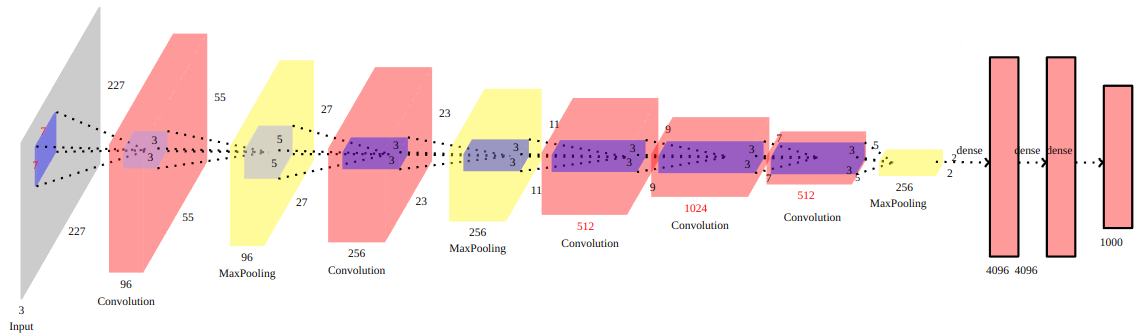
\includegraphics[width=350pt]{50}
	\centering
	\caption{Architecture of ZFNet}
\end{figure}

\subsection{VGGNet}
The VGGnet, introduced in 2014, has earned widespread acclaim and popularity within the domain of Convolutional Neural Networks (CNNs), despite not clinching the top position in the ImageNet Large Scale Visual Recognition Challenge (ILSVRC) of 2014.

What distinguishes the VGGnet and contributes to its widespread adoption is its commitment to model simplicity and the strategic use of small-sized convolutional kernels. This design choice results in the development of exceptionally deep networks, a feature that has resonated well with the research community and practitioners alike.

The authors of VGGnet proposed a range of network configurations, among which the D and E configurations, commonly referred to as VGGnet-16 and VGGnet-19, have emerged as the most successful iterations. These configurations are characterized by their depth and have become benchmarks in the field of deep learning.

The key architectural feature of VGGnet lies in its strict utilization of 3x3 convolutional kernels. This consistent choice of kernel size is complemented by intermediate maxpooling layers, strategically incorporated for effective feature extraction. Toward the end of the architecture, a sequence of three fully connected layers is employed for the final stages of classification.

The success of VGGnet can be attributed to its emphasis on simplicity, the efficacy of small convolutional kernels, and the establishment of well-defined architectures like VGGnet-16 and VGGnet-19. These attributes have contributed to VGGnet's enduring popularity and its continued influence on the design principles of subsequent CNN models.
\begin{figure}[ht]
	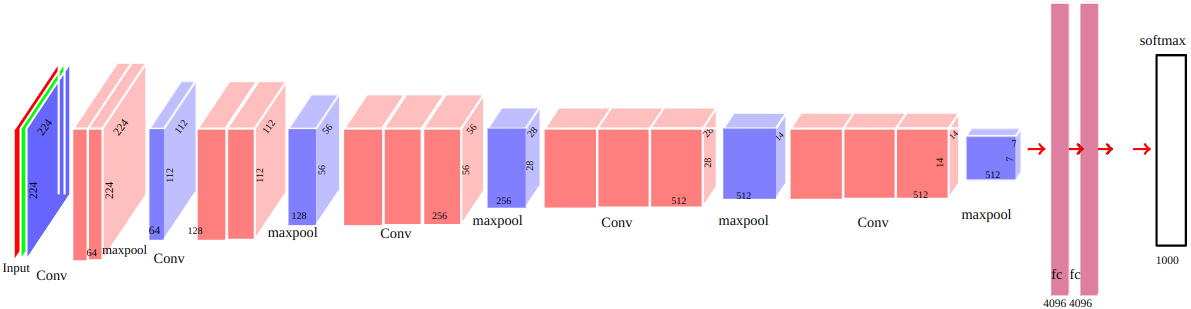
\includegraphics[width=350pt]{51}
	\centering
	\caption{Architecture of VGGNet}
\end{figure}

\subsection{GoogleNet (Previously Inception)}
GoogleNet, formally known as Inception, represents a notable advancement in the realm of Convolutional Neural Networks (CNNs) and was introduced in 2014. Developed by researchers at Google, particularly Christian Szegedy et al., GoogleNet stands out for its innovative architectural design, addressing challenges associated with computational efficiency and model interpretability.

The primary motivation behind GoogleNet was to create a network that achieves high accuracy while maintaining computational efficiency. The architecture introduced a novel concept known as the "Inception module," which significantly contributed to achieving this goal.

The Inception module is characterized by its use of multiple filter sizes, including 1x1, 3x3, and 5x5 convolutional filters, as well as pooling operations, within the same layer. By incorporating diverse filter sizes, the model can capture features at different scales and hierarchies, enhancing its ability to learn complex representations from the input data.

Additionally, GoogleNet employs a parallel structure in its architecture, utilizing multiple Inception modules in parallel and concatenating their outputs. This parallelism allows the model to capture a rich variety of features, promoting better generalization and representation learning.

To address the computational challenge associated with increased depth, GoogleNet incorporates 1x1 convolutions as dimensionality reduction layers before the 3x3 and 5x5 convolutions. This helps in reducing the number of input channels and consequently lowers the computational cost.

In terms of model interpretability, GoogleNet introduced the concept of auxiliary classifiers. These auxiliary classifiers are placed at intermediate layers of the network and contribute to the overall loss during training. They serve the dual purpose of providing additional supervision to the model during training and addressing the vanishing gradient problem.


\begin{figure}[ht]
	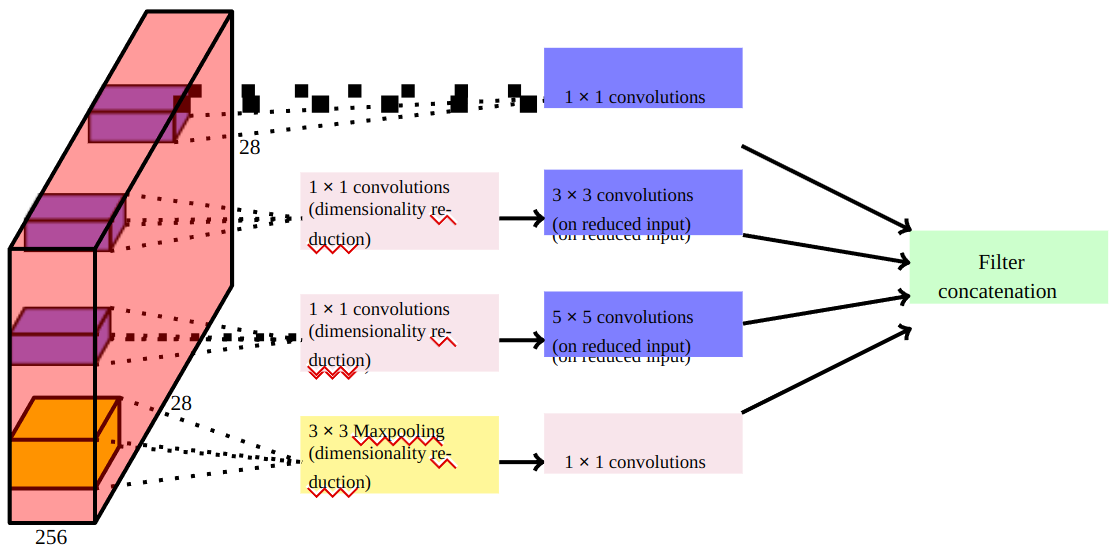
\includegraphics[width=350pt]{52}
	\centering
	\caption{Inception module}
\end{figure}

\begin{figure}[ht]
	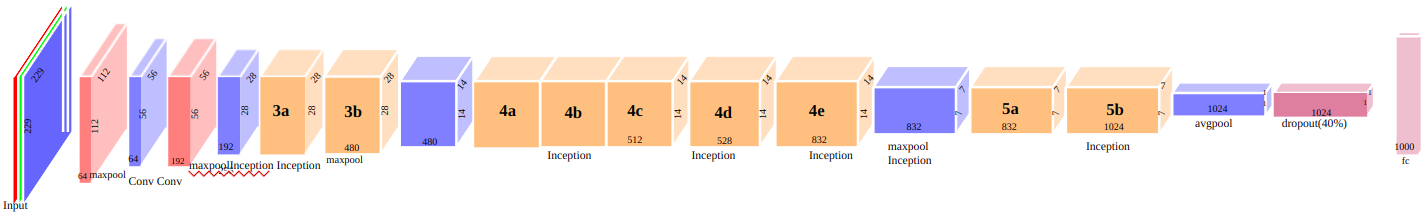
\includegraphics[width=350pt]{53}
	\centering
	\caption{GoogleNet Architecture}
\end{figure}

\subsection{ResNet}

ResNet, short for Residual Network, is a groundbreaking convolutional neural network (CNN) architecture that was introduced in 2015 by Kaiming He, Xiangyu Zhang, Shaoqing Ren, and Jian Sun. ResNet stands out for its innovative use of residual learning, which addresses challenges associated with training very deep networks by introducing shortcut connections or skip connections.

The core idea behind ResNet is to tackle the vanishing gradient problem that often occurs when training deep neural networks. As the depth of the network increases, traditional architectures face difficulties in effectively propagating gradients during backpropagation, hindering the learning process. ResNet mitigates this issue by introducing residual blocks, allowing the network to learn residual functions.

A residual block consists of a shortcut connection that skips one or more layers, combined with the output of the layer(s) it bypasses. This approach enables the network to learn the residual mapping between the input and output of a block, making it easier to optimize the learning process for very deep architectures.

The architecture's deep residual learning enables the construction of exceptionally deep networks, surpassing the limitations of previous designs. ResNet is known for its scalability, and it has been successfully applied to a wide range of computer vision tasks, including image classification, object detection, and segmentation.

ResNet architectures come in various depths, with ResNet-50 and ResNet-101 being popular configurations. These numbers correspond to the number of layers in the network, reflecting the network's ability to handle increasingly complex hierarchical features.

Here are the bag of tricks used my ResNet that makes it an award winning model:
\begin{enumerate}
\item Batch Normalization after Every Convolutional Layer: Batch normalization is applied after every convolutional layer to mitigate internal covariate shift and enhance stability during training.

\item Xavier/2 Initialization from [He et al] Xavier (Glorot) initialization is used, specifically the "Xavier/2" initialization, which scales weights according to the square root of the number of input units to prevent vanishing or exploding gradients.

\item SGD + Momentum (0.9): Stochastic Gradient Descent (SGD) is used with a momentum term set to 0.9 for faster convergence by introducing a moving average of past gradients.

\item Learning Rate: 0.1, Divided by 10 when Validation Error Plaeuus: The initial learning rate is set to 0.1, and it is divided by 10 when the validation error plateaus to fine-tune the learning process.

\item Mini-batch Size 256: A mini-batch size of 256 is used, indicating that 256 samples are processed in each training iteration.

\item Weight Decay of 1e-5: Weight decay of 1e-5 is applied as a regularization technique to penalize large weights and encourage simpler model solutions.

\item No Dropout Used: No dropout is employed as a regularization technique, suggesting that other methods and architectural choices suffice for preventing overfitting.
\end{enumerate}

\begin{figure}[ht]
	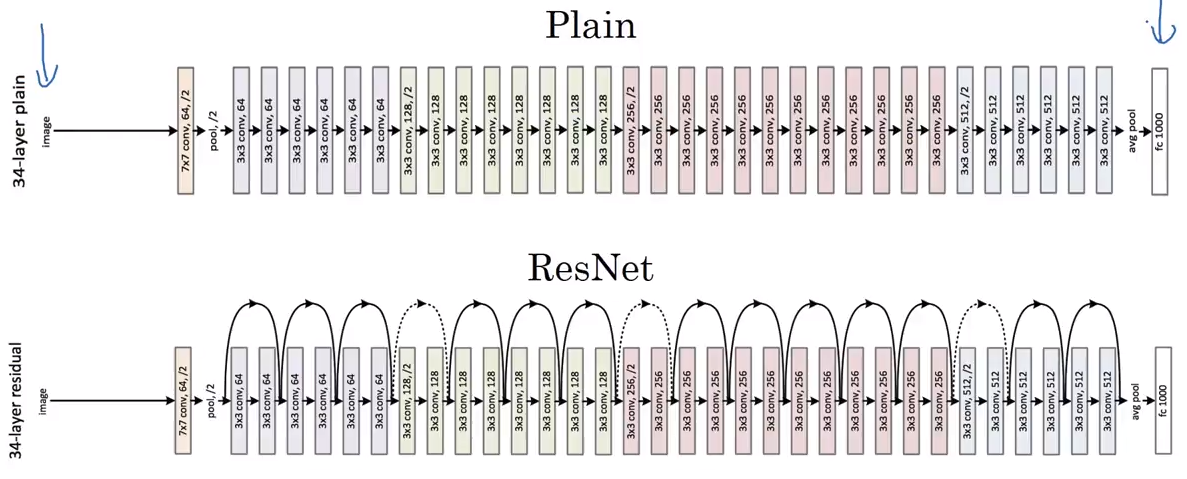
\includegraphics[width=350pt]{54}
	\centering
	\caption{ResNet Architecture}
\end{figure}

\chapter{Recurrent Neural Networks, Transformers and Attention}

\section{Sequential Data}
Sequential data refers to a type of data where the order of elements is significant and holds intrinsic meaning. Unlike non-sequential data, such as tabular data, where each entry is independent of its position, sequential data relies on the arrangement of elements to convey information.

The key distinguishing feature of sequential data lies in the temporal or spatial relationships between its constituent elements. These relationships establish patterns, dependencies, and structures that are crucial for understanding the underlying information.

Here are some examples for understanding what sequential data may look like:
\begin{itemize}
	\item \textbf{Time Series Data:} Perhaps the quintessential example of sequential data, time series data represents observations collected over time, such as stock prices, weather conditions, or physiological measurements.
\item \textbf{Textual Data:} Written language inherently follows a sequential structure, making text data an evident example. Sentences, paragraphs, and chapters convey meaning through the order of words and phrases. 
\item \textbf{DNA Sequences:} In bioinformatics, genetic information is often represented as sequences of nucleotides. The order of these nucleotides is fundamental in understanding genetic codes and functionalities.
\item \textbf{Clickstream Data:} User interactions on websites or applications generate clickstream data. The sequence of clicks, page views, and interactions is crucial for analyzing user behavior and optimizing user experience.
\item \textbf{Speech Signals:} Audio data, particularly speech signals, is inherently sequential. The sequence of phonemes and words conveys the spoken message, making it an essential form of sequential data.

\item \textbf{Gesture Recognition:} In computer vision, sequences of gestures or movements are often analyzed to interpret human actions. The temporal order of these gestures is vital for accurate recognition.
\end{itemize}

In sequence modeling there can be different mappings between input and output sequences. These mappings define the relationship between the lengths of input and output sequences. These different mappings allow for flexibility in addressing various types of problems in sequence modeling, ranging from simple one-to-one relationships to more complex scenarios involving multiple inputs and outputs. The choice of the mapping depends on the nature of the task and the characteristics of the data.

\begin{enumerate}
	\item \textbf{One-to-One} (1:1): In a one-to-one sequence model, each element in the input sequence corresponds to exactly one element in the output sequence.
Example: Traditional feedforward neural networks, where each input feature has a direct correspondence to an output.
\item \textbf{One-to-Many} (1:N): A single input element is used to generate multiple output elements.
Example: Image captioning, where an image is the input, and the model generates a sequence of words describing the image.

\item \textbf{Many-to-One} (N:1): Multiple input elements are used to generate a single output element.
Example: Sentiment analysis in natural language processing, where a sequence of words is the input, and the model outputs the sentiment of the entire sequence.
Many-to-Many (N:N):

\item \textbf{Many-to-Many} (N:N): Both input and output sequences have multiple elements, and there is a many-to-many relationship between them. The lengths of the input and output sequences may or may not be the same.
Example: Language translation, where a sequence of words in one language is translated into a sequence of words in another language. The input and output sequences can have different lengths.
\end{enumerate}

\begin{figure}[ht]
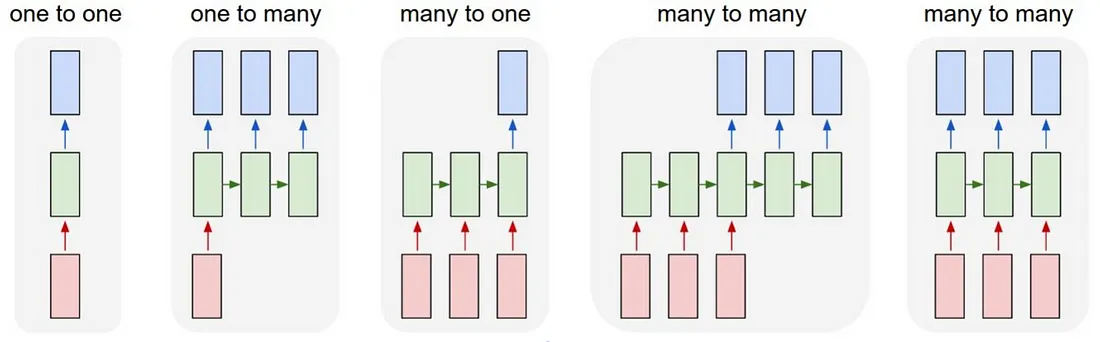
\includegraphics[width=350pt]{32}
\centering
\caption{Different mappings between inputs and outputs in sequence modelling}
\end{figure}

\section{Sequence Modeling}

\begin{figure}[ht]
	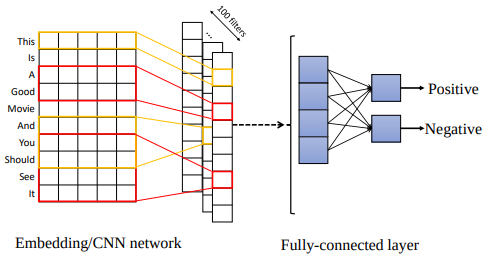
\includegraphics[width=250pt]{33}
	\centering
	\caption{A general architecture of 1D CNN based text classification}
\end{figure}
On a basic level, interpreting a certain part of a sequence requires information gained from the previous parts of the sequence. RNNs try to incorporate this capacity of memory by updating the “state” of its cells each time we move from one part of a sequence to another. The state of a cell is basically the total information gained by it so far by reading the sequence. So, the current state or knowledge of a cell in an RNN is not only dependent on the current word or sentence it is reading, but is also dependent on all the other words or sentences it has read before the current one.

To go from multi-layer networks to recurrent networks, we need to take advantage of parameter sharing. Parameter sharing makes it possible to extend and apply the model to examples of different forms (different lengths) and generalize across them. When we attempt to generalize over a sequence, the sequence length of the input may not be fixed and will often not be seen during the training phase. Further more, the statistical strength must be shared across different time different positions in time to make sense of the sequence. This is gravely evident in semantics of languages. For instance the sentence "In 2009, I went to Nepal" and "I went to Nepal in 2009" are both semantically equivalent but the time steps of information are different. It is also to be noted that two time steps can be related (like how nepal and 2009 are related here) and to compute these relations the model must learn all of these liguistic rules.

The first related idea to use of convolution across a 1-D temporal sequence. This convolutional approach is the basis for time-delay neural networks. The convolution operation allows a network to share parameters across time, but is shallow. The output of convolution is a sequence where each member of the output is a function of a small number of neighboring members of the input. The idea of parameter sharing manifests in the application of the same convolution kernel at each time step.


Recurrent networks share parameters in a different way. Each member of the output is a function of the previous members of the output. Each member of the output is produced using the same up date rule applied to the previous outputs. This recurrent formulation results in the sharing of parameters through a very deep computational graph.

\section{Recurrent Neural Networks}

To understand the architecture of an RNN we extend to the concept of computational graphs. A computational graph is a way to formalize the structure of a set of computations, such as those involved in mapping inputs and parameters to outputs and loss. A Recurrent Neural Network as the name suggests includes cycles in it's computational graph. These cycles represent the influence of the present value of a variable on its own value at a future time step. 

\begin{figure}[ht]
	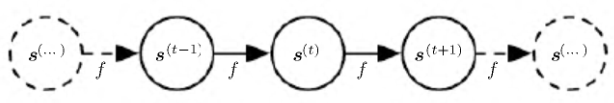
\includegraphics[width=250pt]{34}
	\centering
	\caption{Unfolding graph of an RNN. Each node represents the state at some timet and the function $f$ maps the state at $t$ to the state at $t + 1$. The same parameters (the same value of used to parametrize) are used for all time steps.}
\end{figure}

For example, consider the classical form of a dynamical system:
$$s^{(t)} = f(s^{(t-1)}; \theta)$$
where: \\ 
$s^{(t)}$ is called the state of the system.

For a finite number of time steps $\tau$, the graph can be unfolded by applying the definition $\tau - 1$ times. For example, if we unfold equation for $\tau=3$ time steps (Fig 4.3), we obtain:

$$s^{(3)} = f(s^{(2)}; \theta) = f(s^{(1)}; \theta) $$

Unfolding the equation by repeatedly applying the definition in this way has yielded an expression that does not involve recurrence. Such an expression can now be represented by a traditional directed acyclic computational graph as illustrated in the Fig 4.3.

Let us consider a dynamical system driven by an external signal $x^{(t)}$.
$$s^{(t)} = f(s^{(t-1)}, x; \theta)$$

We rewrite  the equation with $h$ representing the state to indicate that the state is the hidden
units of the network.
$$h^{(t)} = f(h^{(t-1)}, x; \theta)$$

Finally, typical RNNs will add extra architectural features such as output layers that read information out of the state $h$ to make predictions.

When the recurrent network is trained to perform a task that requires predicting the future from the past, the network typically learns to use $h^{(t)}$ as a kind of lossy summary of the task-relevant aspects of the past sequence of inputs up to $t$. This summary is in general necessarily lossy, since it maps an arbitrary length sequence $\lt( x^{(t)}, x^{(t-1)}, x^{(t-2)}, \cdots, x^{(2)}, x^{(1)}\rt)$ to a fixed length vector $h^{(t)}$. Depending on the training criterion, this summary might selectively keep some aspects of the past sequence with more precision than other aspects.

\begin{figure}[ht]
	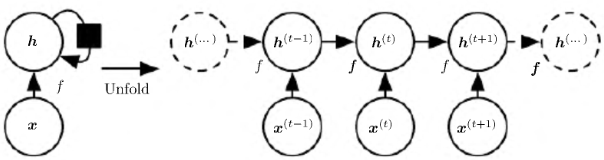
\includegraphics[width=300pt]{35}
\centering
\caption{A recurrent network with no outputs. This recurrent network just processes information from the input $x$ by incorporating it into the state $h$ that is passed forward through time. (Left) Circuit diagram. The black square indicates a delay of a single time step. The same network seen as an unfolded computational graph, where each (Right) node is now associated with one particular time instance.}
\end{figure}

We can represent the unfolded recurrence after steps with a function $g^{(t)}$:
$$h^{(t)} = g^{(t)} ( x^{(t)} + x^{(t-1)} \cdots x^{(2)} + x^{(1)})$$
$$h^{(t)} = f(h^{(t - 1)}, x^{(t)}; \theta)$$

The function $g^{(t)}$ takes the whole past sequence $(x^{(t)}, x^{(t-1)}, x^{(t-2)} \cdots x^{(2)}, x^{(1)})$
as input and produces the current state, but the unfolded recurrent structure
allows us to factorize $g^{(t)}$ into rep eated application of a function $f$. The unfolding
process thus introduces two major advantages:
\begin{enumerate}	
	\item Regardless of the sequence length, the learned model always has the same input size, because it is specified in terms of transition from one state to another state, rather than specified in terms of a variable-length history of states.
	\item It is possible to use the transition function same $f$ with the same parameters at every time step. 

	\end{enumerate}
These two factors make it possible to learn a single model $f$ that op erates on all time steps and all sequence lengths, rather than needing to learn a separate model $g^{(t)}$ for all possible time steps. Learning a single, shared model allows generalization to sequence lengths that did not appear in the training set, and allows the model to b e estimated with far fewer training examples than would be required without parameter sharing.

This concludes that any function that is computable by a Turing machine can be computed by a recurrent neural network of a finite size.

Armed with the graph unrolling and parameter sharing ideas of section ,we can design a wide variety of recurrent neural networks.
\begin{figure}[ht]
	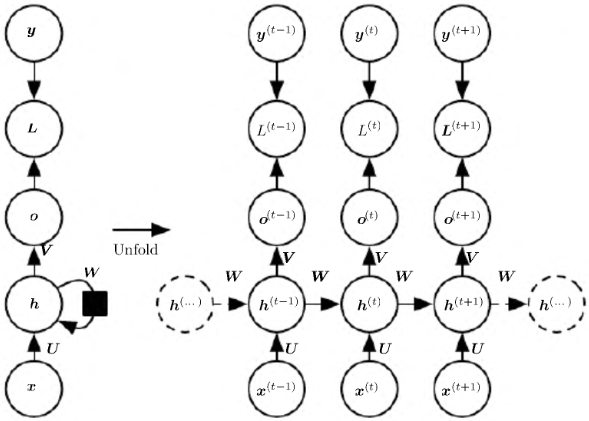
\includegraphics[width=250pt]{36}
	\centering
	\caption{Recurrent networks that produce an output at each time step and have recurrent connections between hidden units}
\end{figure}

\begin{figure}[ht]
	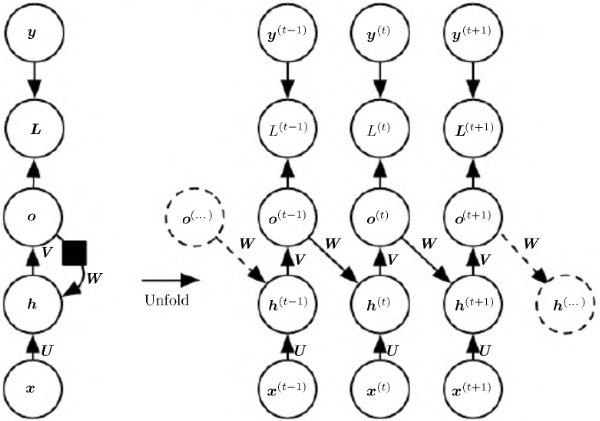
\includegraphics[width=250pt]{37}
	\centering
	\caption{Recurrent networks that produce an output at each time step and have recurrent connections only from the output at one time step to the hidden units at the next time step,}
\end{figure}

\begin{figure}[ht]
	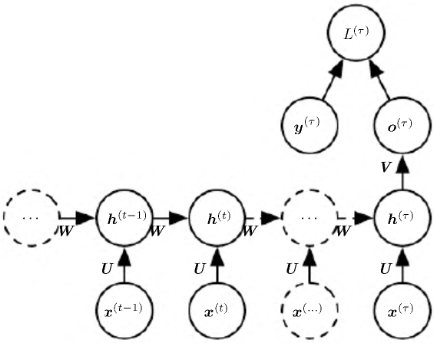
\includegraphics[width=250pt]{38}
	\centering
	\caption{Recurrent networks with recurrent connections between hidden units, that read an entire sequence and then produce a single output}
\end{figure}

We now develop the forward propagation equations for the RNN depicted in figure 4.5. The figure does not specify the choice of activation function for the hidden units. Here we assume the hyperbolic tangent activation function. Also, the figure does not specify exactly what form the output and loss function take. Here we assume that the output is discrete, as if the RNN is used to predict words or characters. A natural way to represent discrete variables is to regard the output $o$ as giving the unnormalized log probabilities of each possible value of the discrete variable. We can then apply the softmax operation as a post-pro cessing step to obtain a vector $\hat{y}$ of normalized probabilities over the output. Forward propagation begins with a sp ecification of the initial state $h^{(0)}$. Then, for each time step from $t$ to $\tau$:
\\
$a^{(t)} = b + \mathbf{W}h^{(t-1)} + \mathbf{U}x^{(t)}$
$h^{(t)} = \text{tanh}(a^{(t)})$ \\
$o^{(t)} = c + \mathbf{V}h^{(t)}$ \\
$\hat{y}^{(t)} = \text{softmax}(o^{(t)})$
 
where the parameters are the bias vectors $b$ and $c$ along with the weight matrices $\mathbf{U}$ , $\mathbf{V}$ and $\mathbf{W}$ , respectively for input-to-hidden, hidden-to-output and hidden-to-hidden connections. This is an example of a recurrent network that maps an input sequence to an output sequence of the same length. The total loss for a given sequence of $x$ values paired with a sequence of values would then be just $y$ the sum of the losses over all the time steps. For example, if $L^{(t)}$ is the negative log-likelihood of $y^{(t)}$ given $x^{(t)}, \cdots , x^{(t)}$ , then

$$L\lt(\{x^{(1)}, \cdots, x^{(\tau)}\}, \{y^{(1)}, \cdots, y^{(\tau)}\}\rt) = \sum_t L^{(t)}$$
$$= - \sum_t log p_{\text{model}}\lt(y^{(t)} | x^{(1)}, \cdots, x^{(t)}\rt)$$

where $p_\text{model}$ $(y^{(t)} | \{x^{(1)}, \cdots, x^{(t)}\})$ is given by reading the entry for $y^{(t)}$ from the model’s output vector $\hat{y^{(t)}}$

\section{RNN from scratch}
\begin{verbatim}
import torch
import torch.nn as nn

class RNNClass(nn.Module):
    def __init__(self, input_size, hidden_size, output_size):
        super(RNNClass, self).__init__()
        
        self.hidden_size = hidden_size
        
        # Define the RNN layer
        self.rnn = nn.RNN(input_size, hidden_size, batch_first=True)
        
        # Define the output layer
        self.fc = nn.Linear(hidden_size, output_size)
        
    def forward(self, x):
        # Initialize hidden state with zeros
        h0 = torch.zeros(1, x.size(0), self.hidden_size).to(x.device)
        
        # Forward pass through the RNN layer
        out, _ = self.rnn(x, h0)
        
        # Take the output from the last time step
        out = self.fc(out[:, -1, :])
        
        return out

# Example usage:
input_size = 10
hidden_size = 20
output_size = 5

# Create an instance of the RNNClass class
rnn_model = RNNClass(input_size, hidden_size, output_size)

# Sample input tensor
sample_input = torch.randn(3, 15, input_size)  # (batch_size, sequence_length, input_size)

# Forward pass
output = rnn_model(sample_input)

print("Input size:", sample_input.size())
print("Output size:", output.size())
\end{verbatim}

\section{Teacher Forcing and Networks with Output Reference} 
\begin{figure}[ht]
	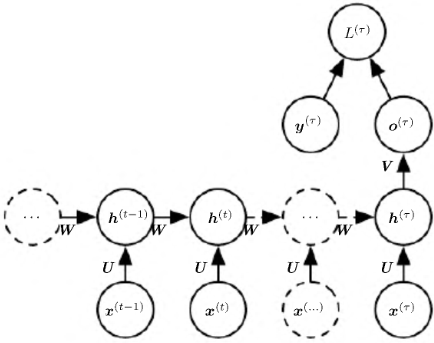
\includegraphics[width=250pt]{39}
	\centering
	\caption{Time-unfolded recurrent neural network with a single output at the end of the sequence. Such a network can be used to summarize a sequence and produce a fixed-size representation used as input for further processing. There might be a target right at the end (as depicted here) or the gradient on the output $o^{(t)}$ can be obtained by back-propagating from further downstream modules.}
\end{figure}

The network with recurrent connections only from the output at one time step to the hidden units at the next time step is strictly less powerful because it lacks hidden-to-hidden recurrent connections. For example, it cannot simulate a universal Turing machine. Because this network lacks hidden-to-hidden recurrence, it requires that the output units capture all of the information about the past that the network will use to predict the future.

The advantage of eliminating hidden-to-hidden recurrence is that, for any loss function based on comparing the prediction at time $t$ to the training target at time $t$, all the time steps are decoupled. Training can thus b e parallelized, with the gradient for each step $t$ computed in isolation. There is no need to compute the output for the previous time step first, because the training set provides the ideal value of that output.

Models that have recurrent connections from their outputs leading back into the model may be trained with teacher forcing. Teacher forcing is a procedure that emerges from the maximum likelihood criterion, in which during training the model receives the ground truth output $y^{(t)}$ as input at time $t+1$. We can see this by examining a sequence with two time steps.

\begin{figure}[ht]
	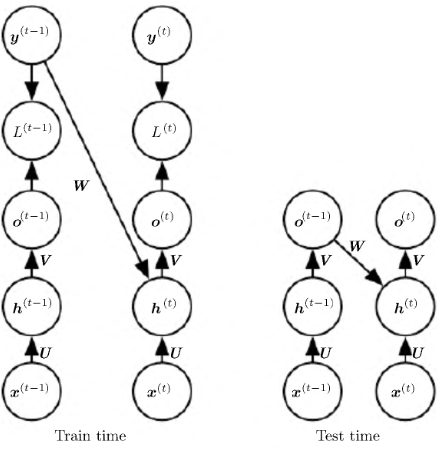
\includegraphics[width=250pt]{40}
	\centering
	\caption{Illustration of teacher forcing. Teacher forcing is a training technique that is applicable to RNNs that have connections from their output to their hidden states at the next time step. (Left)At train time, we feed the correct output $y^{(t)}$ drawn from the train set as input to $h^{(t+1)}$.(Right)When the model is deployed, the true output is generally not known. In this case, we approximate the correct output $y^{(t)}$ with the model’s output $o^{(t)}$, and feed the output back into the model.}
\end{figure}

\textbf{Advantages}:
\begin{enumerate}
\item \textbf{Faster Convergence}: Teacher forcing can lead to faster convergence during training. By providing the model with ground truth values at each step, it helps guide the learning process and stabilize the training dynamics.

\item \textbf{Reduced Training Time}: Training with teacher forcing often requires fewer iterations to achieve satisfactory results compared to training without it. This can be particularly advantageous when computational resources are limited.

\item \textbf{Stable Training}: The teacher forcing method provides a stable and well-defined training signal, especially in the early stages of training. This can help the model learn dependencies and relationships in the data more effectively.

\item \textbf{Easier Implementation}: Implementing teacher forcing is relatively straightforward. It involves supplying the true target values as inputs during training, simplifying the training procedure.

\item \textbf{Handling Variable-Length Sequences}: Teacher forcing can handle variable-length input sequences more easily than other methods. This makes it suitable for tasks where input sequence lengths vary across examples.
\end{enumerate}

\textbf{Disadvantages}:
\begin{enumerate}
\item \textbf{Exposure Bias}: One of the main drawbacks of teacher forcing is exposure bias. The model becomes accustomed to the ground truth values during training, and when it is deployed for inference, where true values are unavailable, it may struggle to generate accurate predictions.

\item \textbf{Mismatch between Training and Inference}: Due to exposure bias, there can be a significant mismatch between the training and inference phases. This can result in suboptimal performance during actual use.

\item \textbf{Inaccurate Long-Term Predictions}: Teacher forcing may lead to inaccurate long-term predictions. The model may struggle to generate sequences beyond the training context, as it relies heavily on the ground truth values provided during training.

\item \textbf{Difficulty in Capturing Uncertainty}: Teacher forcing may not effectively capture the uncertainty inherent in the generation process. The model might become overly confident in its predictions, even when there is significant uncertainty in the data.

\item \textbf{Limitations in Sequential Decision-Making}: In tasks involving sequential decision-making, such as reinforcement learning, the deterministic nature of teacher forcing may limit the model's ability to explore alternative trajectories.
\end{enumerate}

We originally motivated teacher forcing as allowing us to avoid back-propagation through time in models that lack hidden-to-hidden connections. Teacher forcing may still be applied to models that have hidden-to-hidden connections so long as they have connections from the output at one time step to values computed in the next time step. However, as so on as the hidden units b ecome a function of earlier time steps, the BPTT algorithm is necessary. Some models may thus be trained with both teacher forcing and BPTT.

\subsection{Professor Forcing}

Professor forcing is a new training technique for RNNs that is inspired by adversarial domain adaptation. In adversarial domain adaptation, two networks are trained in an adversarial manner: a discriminator network that tries to distinguish between the source domain and the target domain, and a generator network that tries to generate samples that are indistinguishable from the target domain. Professor forcing uses a similar setup, but instead of two networks, it uses a single network that is trained to distinguish between the dynamics of the network when training the network and when sampling from the network over multiple time steps.

Regular teacher forcing has two main drawbacks:

\begin{enumerate}
	\item It can lead to overfitting, as the network may become too reliant on the ground truth values.

	\item It can make it difficult to generate long-range sequences, as the network may not be able to learn how to propagate information over long distances.
\end{enumerate}

Professor forcing addresses both of these drawbacks. By training the network to distinguish between its own dynamics during training and sampling, professor forcing encourages the network to learn how to propagate information over long distances. This can improve the accuracy of the network's predictions on long-range sequences. Additionally, professor forcing reduces the risk of overfitting by making the network less reliant on the ground truth values.

Professor Forcing attempts to bridge the gap between training and inference by making the training procedure more aligned with the inference process. Here's how Professor Forcing works:
\begin{enumerate}
	\item \textbf{Training with Scheduled Sampling}: Instead of always using ground truth values during training (as in teacher forcing), Professor Forcing introduces a scheduled sampling mechanism. At each time step during training, there's a probability $p$ of using the ground truth values, and $1-p$ of using the model's own predictions from the previous time step as inputs for the next.

	\item \textbf{Gradual Exposure to Model's Output}: By using the model's own predictions with a certain probability, Professor Forcing exposes the model to its own generated outputs during training. This gradually introduces the model to the discrepancies between its predictions and the ground truth, mimicking the conditions it will face during inference.

\item \textbf{Adaptive Exposure to Reduce Exposure Bias}: The probability $p$ can be annealed or adjusted during training. Initially, $p$ might be high, allowing the model to rely more on ground truth values. As training progresses, $p$ can be decreased, increasing the reliance on the model's own predictions. This adaptive exposure helps mitigate exposure bias.
\end{enumerate}

Professor forcing is a promising new training technique for RNNs that addresses the drawbacks of regular teacher forcing. It has been shown to improve the accuracy of RNNs on a variety of tasks, and it is a promising technique for training RNNs that are used to model long-range or noisy sequential data.

The term "Professor Forcing" is used metaphorically to describe the model learning from both the "professor" (ground truth) and itself during training, preparing it for real-world scenarios where ground truth is not available during inference.

\section{Representing language to a Neural Network}
Neural networks essentially carry out mathematical operations. Thus to pass any form of data into a neural network it is needed that the data must be encoded into numerical data. One-hot embedding is a technique used in machine learning to represent categorical data, such as words or characters, as numeric vectors.

In one-hot embedding, each unique category is assigned a unique integer index. For example, if we have a vocabulary of five words: ["apple", "banana", "cherry", "orange", "pear"], we can assign each word a unique index as follows: {"apple": 0, "banana": 1, "cherry": 2, "orange": 3, "pear": 4}.

To represent a given word in this vocabulary as a vector, we create a vector of zeros of length equal to the size of the vocabulary, and set the value of the element at the index corresponding to the word to 1. For example, the one-hot embedding for the word "banana" would be [0, 1, 0, 0, 0].

One of the advantages of one-hot embedding is its simplicity and interpretability, as each dimension of the vector corresponds to a specific category. However, it can also be very high-dimensional and sparse, which can be computationally expensive and make it difficult to capture relationships between categories.

\section{Computing the Gradient in a Recurrent Neural Network}
Computing the gradient through a recurrent neural network is straightforward. One simply applies the generalized back-propagation algorithm to the unrolled computational graph. No specialized algorithms are necessary. Gradients obtained by back-propagation may then be used with any general-purpose gradient-based techniques to train an RNN. This method of calculating gradients is called Back Propagation Through Time (BPTT).

Backpropagation Through Time (BPTT) is a method used to train Recurrent Neural Networks (RNNs) by backpropagating the error gradient through the entire sequence of the input data. During training, the RNN is first fed with a sequence of input data, which is processed one time step at a time. The output of the network at each time step is compared to the target output, and the difference between them is calculated as the error. The goal of training is to adjust the weights of the RNN so that the error is minimized.

To achieve this, BPTT uses a process similar to the standard backpropagation algorithm used to train feedforward neural networks. In BPTT, the error gradient is first computed at the final time step of the sequence, and then propagated backwards through time to all the previous time steps, one step at a time. At each time step, the error gradient is multiplied by the derivative of the activation function and then backpropagated to the previous time step, where it is accumulated with the gradients from the subsequent time steps. This process is repeated until the gradient has been backpropagated through the entire sequence. Once the gradient has been computed, it is used to update the weights of the RNN using an optimization algorithm such as gradient descent. This process is repeated for multiple epochs until the network is trained to minimize the error.

In an RNN, the same set of weights is used across all time steps in the sequence. During backpropagation, the gradients for these weights are computed by multiplying the gradients at each time step by the weights. However, if the gradients at each time step are small, their product will become exponentially smaller as it propagates through time, leading to a vanishing gradient problem. This is why it is said that RNNs suffer from a short term memory issue.

The nodes of our computational graph include the parameters $\mathbf U$ , $\mathbf V$ , $\mathbf W$ , $b$ and $c$ as well as the sequence of nodes indexed by $t$ for $x^{(t)}$, $h^{(t)}$, $o^{(t)}$ and $L^{(t)}$.For each node $N$ we need to compute the gradient $\nabla_N{L}$ recursively, based on the gradient computed at nodes that follow it in the graph. We start the recursion with the no des immediately preceding the final loss:
$$\frac{\partial L}{\partial{ L^{(t)}}} = 1$$

The gradient on all parameters are given by:

$	\nabla_c L = \sum_t \lt(\frac{\partial o^{(t)}}{\partial c}\rt)^\top \nabla_{o^{(t)}} L = \sum_t \nabla_{o^{(t)}} L$ \\
$	\nabla_b L = \sum_t \lt(\frac{\partial h^{(t)}}{\partial b^{(t)}}\rt)^\top \nabla_{h^{(t)}}L = \sum_t \text{diag}\lt(1-\lt(h^{(t)}\rt)^2\rt) \nabla_{h^{(t)}} L$ \\
	$\nabla_V L = \sum_t \sum_i \lt(\frac{\partial L}{\partial o_i^{(t)}}\rt) \nabla_{V}o_i^{(t)} = \sum_t (\nabla_{o^{(t)}} L) h^{(t)\top}$ \\
	$\nabla_W L = \sum_t \sum_i \lt(\frac{\partial L}{\partial h_i^{(t)}}\rt) \nabla_{W^{(t)}}h_i^{(t)}$ \\
	$= \sum_t \text{diag}\lt(1-\lt(h^{(t)}\rt)^2\rt)(\nabla_{h^{(t)}}L)h^{(t-1)\top}$ \\
	$\nabla_U L = \sum_t \sum_i \lt(\frac{\partial L}{\partial h_i^{(t)}}\rt) \nabla_{U^{(t)}}h_i^{(t)}$ \\
	$ = \sum_t \text{diag}\lt(1-\lt(h^{(t)}\rt)^2\rt)(\nabla_{h^{(t)}}L)x^{(t)\top}$ 
 
	We do not need to compute the gradient with respect to $x^{(t)}$ for training because it does not have any parameters as ancestors in the computational graph defining the loss.

\section{Bidirectional RNNs}
All of the recurrent networks we have considered up to now have a “causal” structure, meaning that the state at time t only captures information from the past, $x^{(1)},\cdots,x^{(t-1)}$ , and the present input $x^{(t)}$. Some of the models we have discussed also allow information from past y values to affect the current state when the y values are available. However, in many applications we want to output a prediction of $y^{(t)}$ which may depend on the whole input sequence.

For example, in speech recognition, the correct interpretation of the current sound as a phoneme may depend on the next few phonemes because of co-articulation and potentially may even depend on the next few words because of the linguistic dependencies between nearby words: if there are two interpretations of the current word that are both acoustically plausible, we may have to look far into the future (and the past) to disambiguate them.

\begin{figure}[ht]
	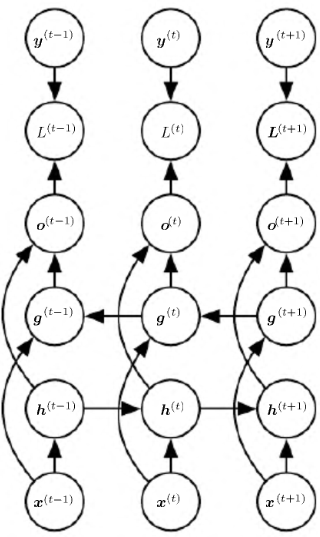
\includegraphics[width=250pt]{41}
	\centering
	\caption{Computation of a typical bidirectional recurrent neural network, meant to learn to map input sequences $x$ to target sequences $y$, with loss $L^{(t)}$ at each step $t$.}
\end{figure}

As the name suggests, bidirectional RNNs combine an RNN that moves forward through time beginning from the start of the sequence with another RNN that moves backward through time beginning from the end of the sequence.

The typical bidirectional RNN, with $h^{(t)}$ standing for the state of the sub-RNN that moves forward through time and $g^{(t)}$  standing for the state of the sub-RNN that moves backward through time. This allows the output units $o^{(t)}$ to compute a representation that depends on both the past and the future but is most sensitive to the input values around time $t$, without having to specify a fixed-size window around $t$ (as one would have to do with a feedforward network, a convolutional network, or a regular RNN with a fixed-size look-ahead buffer).

\section{Encoder-Decoder Sequence-to-Sequence Architecture}
Here we discuss how an RNN can b e trained to map an input sequence to an output sequence which is not necessarily of the same length. This comes up in many applications, such as speech recognition, machine translation or question-answering, where the input and output sequences in the training set are generally not of the same length (although their lengths might be related).

We often call the input to the RNN the “context.” We want to produce a representation of this context, $C$. The context $C$ might be a vector or sequence of vectors that summarize the input sequence $X = (x^{(1)}, \cdots, x^{(n_x)})$.

\begin{figure}[ht]
	\includegraphics[width=250pt]{42}
	\centering
	\caption{Example of an enco der-decoder or sequence-to-sequence RNN architecture,for learning to generate an output sequence $(y^{(1)}, \cdots, y^{n_y})$ given an input sequence $(x^{(1)} ,x^{(2)} ,\cdots,x^{n_x})$. It is composed of an encoder RNN that reads the input sequence and a decoder RNN that generates the output sequence (or computes the probability of a  given output sequence). The final hidden state of the encoder RNN is used to compute a generally fixed-size context variable $C$ which represents a semantic summary of the input sequence and is given as input to the decoder RNN.}
\end{figure}
The idea is very simple: 
\begin{enumerate}
	\item an encoder or reader or input RNN processes the input sequence. The encoder emits the context $C$ , usually as a simple function of its final hidden state. 
	\item  a decoder or writer or output RNN is conditioned on that fixed-length vector to generate the output sequence $Y = (y{(1)}, \cdots , y^{(n_y)})$.
\end{enumerate}


\section{Limitations of RNN}
While RNNs are powerful and have achieved remarkable success in many tasks, they also have some limitations, including:
\begin{enumerate}
	\item Gradient vanishing/exploding: When training RNNs, the gradients can become very small or very large, making it difficult to train the model effectively. This can be a particular problem when working with long sequences.

	\item Limited memory: RNNs can only remember a limited amount of context from the past, which can be a problem when working with long sequences or complex patterns.

	\item Difficulty with long-term dependencies: While RNNs are designed to handle sequential data, they can have difficulty with long-term dependencies, meaning that they may not be able to effectively capture relationships between distant elements in a sequence.

	\item Slow training and no parallelization: Training RNNs can be computationally expensive and time-consuming, which can be a problem for large-scale applications or real-time systems.

	\item Difficulty with variable-length input: RNNs are designed to handle sequences of fixed length, which can be a problem when working with data that has variable-length input sequences.

	\item Difficulty with different input types: RNNs are primarily designed to handle sequential data, so they may not be well-suited to other types of data, such as images or graphs.

	\item Overfitting: RNNs can be prone to overfitting when the training data is limited or the model is too complex. This can result in poor generalization performance on new data.
\end{enumerate}

\section{Alleviating the problem of Vanishing Gradient}
The problem of vanishing gradient can be mitigated by adjustment of a few things in our neural network setup.
\begin{enumerate}
	\item \textbf{ReLU activation function:} One of the main causes of the vanishing gradient problem is the use of activation functions with gradients that become too small, such as sigmoid or tanh, especially in deep networks. This can cause the gradients to vanish as they propagate through the network, making it difficult for the network to learn. The ReLU activation function helps to address this problem by having a gradient that is not only non-zero but also constant, for positive values of the input. Specifically, the derivative of ReLU with respect to the input is 1 for positive inputs and 0 for negative inputs. This ensures that the gradients will not vanish as long as the input is positive.
	\item \textbf{Parameter initialization:} To prevent the weights from shrinking to zero we initialize the weights to an identity matrix and biases as zero.
	\item \textbf{Gated Cells:} Gated cells introduce a mechanism for selectively remembering or forgetting information from previous time steps. This helps to prevent the gradients from vanishing or exploding, especially in long sequences, by allowing the network to selectively propagate or block the gradients based on their relevance to the current task. Gated cells introduce a mechanism for addressing the problem of long-term dependencies in the input data. The vanishing gradient problem is particularly pronounced in RNNs because the gradients have to be propagated through multiple time steps, which can result in them becoming too small to be effective. Gated cells, such as LSTMs and GRUs, address this problem by selectively retaining important information from previous time steps and propagating it forward in time.
\end{enumerate}

\section{Long Short Term Memory (LSTM)}
Before the introduction and rise of attention mechanism models used in transformers, the most effective sequence models used in practical applications were gated RNNs. These include the long short-term memory and networks based on the gated recurrent unit. The clever idea of introducing self-loops to produce paths where the gradient can flow for long durations is a core contribution of the initial long short-term memory (LSTM) model.

By making the weight of this self-loop gated (controlled by another hidden unit), the time scale of integration can be changed dynamically. In this case, we mean that even for an LSTM with fixed parameters, the time scale of integration can change based on the input sequence, because the time constants are output by the model itself. The LSTM has been found extremely successful in many applications, such as unconstrained handwriting recognition, speech recognition. handwriting generation, machine translation, image captioning and parsing.

\begin{figure}[ht]
	\includegraphics[width=350pt]{43}
	\centering
	\caption{The LSTM Cell}
\end{figure}

The core concept of LSTM’s are the cell state, and it’s various gates. The cell state act as a transport highway that transfers relative information all the way down the sequence chain. You can think of it as the “memory” of the network. The cell state, in theory, can carry relevant information throughout the processing of the sequence. So even information from the earlier time steps can make it’s way to later time steps, reducing the effects of short-term memory. As the cell state goes on its journey, information get’s added or removed to the cell state via gates. The gates are different neural networks that decide which information is allowed on the cell state. The gates can learn what information is relevant to keep or forget during training.

Gates contains sigmoid activations. A sigmoid activation is similar to the tanh activation. Instead of squishing values between -1 and 1, it squishes values between 0 and 1. That is helpful to update or forget data because any number getting multiplied by 0 is 0, causing values to disappears or be “forgotten.” Any number multiplied by 1 is the same value therefore that value stay’s the same or is “kept.” The network can learn which data is not important therefore can be forgotten or which data is important to keep.

\subsection{Forget Gate}
First, we have the forget gate. This gate decides what information should be thrown away or kept. Information from the previous hidden state and information from the current input is passed through the sigmoid function. Values come out between 0 and 1. The closer to 0 means to forget, and the closer to 1 means to keep.

   \[
   f_t = \sigma(W_{if} x_t + b_{if} + W_{hf} h_{t-1} + b_{hf})
   \]

\subsection{Input Gate}
To update the cell state, we have the input gate. First, we pass the previous hidden state and current input into a sigmoid function. That decides which values will be updated by transforming the values to be between 0 and 1. 0 means not important, and 1 means important. You also pass the hidden state and current input into the tanh function to squish values between -1 and 1 to help regulate the network. Then you multiply the tanh output with the sigmoid output. The sigmoid output will decide which information is important to keep from the tanh output.

Certainly! Long Short-Term Memory (LSTM) networks involve several equations to model their dynamics. Here are the relevant equations in LaTeX format:

   \[
   i_t = \sigma(W_{ii} x_t + b_{ii} + W_{hi} h_{t-1} + b_{hi})
   \]

\subsection{Cell State}
Now we should have enough information to calculate the cell state. First, the cell state gets pointwise multiplied by the forget vector. This has a possibility of dropping values in the cell state if it gets multiplied by values near 0. Then we take the output from the input gate and do a pointwise addition which updates the cell state to new values that the neural network finds relevant. That gives us our new cell state.

Cell Gate (Candidate Values):
   \[
   \tilde{c}_t = \tanh(W_{ig} x_t + b_{ig} + W_{hg} h_{t-1} + b_{hg})
   \]

Cell State Update:
   \[
   c_t = f_t \cdot c_{t-1} + i_t \cdot \tilde{c}_t
   \]

\subsection{Output Gate}
Last we have the output gate. The output gate decides what the next hidden state should be. Remember that the hidden state contains information on previous inputs. The hidden state is also used for predictions. First, we pass the previous hidden state and the current input into a sigmoid function. Then we pass the newly modified cell state to the tanh function. We multiply the tanh output with the sigmoid output to decide what information the hidden state should carry. The output is the hidden state. The new cell state and the new hidden is then carried over to the next time step.

   \[
   o_t = \sigma(W_{io} x_t + b_{io} + W_{ho} h_{t-1} + b_{ho})
   \]

\subsection{Hidden State Update}
   \[
   h_t = o_t \cdot \tanh(c_t)
   \]

\section{Gated Recurrent Unit}
\begin{figure}[ht]
	\includegraphics[width=350pt]{44}
	\centering
	\caption{The GRU Cell}
\end{figure}

The GRU is the newer generation of Recurrent Neural networks and is pretty similar to an LSTM. GRU’s got rid of the cell state and used the hidden state to transfer information. It also only has two gates, a reset gate and update gate.

\subsection{Update Gate}
The update gate acts similar to the forget and input gate of an LSTM. It decides what information to throw away and what new information to add. The update gate functions as a selective filter, regulating the information that is retained and discarded at each time step. Similar to the forget gate in LSTMs, the update gate decides what information from the previous hidden state should be forgotten or preserved. Simultaneously, it plays a role akin to the input gate by determining what new information should be incorporated into the current hidden state. This dual functionality enables GRUs to effectively manage the flow of information over time, allowing the network to learn and remember relevant patterns while discarding less important information. In essence, the update gate serves as a dynamic controller, adaptively updating the hidden state based on the current input and the information deemed valuable from the previous time step.

   \[
   z_t = \sigma(W_{z} x_t + U_{z} h_{t-1} + b_{z})
   \]



\subsection{Reset Gate}
The reset gate is another gate is used to decide how much past information to forget. The reset gate acts as a filter that decides which information is relevant for the current context, helping the model focus on essential features while disregarding less significant details from the past. By doing so, GRUs can capture relevant patterns in sequential data while mitigating the impact of irrelevant or outdated information. This ability is particularly valuable in tasks where understanding temporal dependencies is essential, such as natural language processing and speech recognition.

In essence, the reset gate in GRUs contributes to the model's adaptability, enabling it to dynamically adjust the retention or dismissal of past information based on the current context. This mechanism enhances the network's ability to model and learn from sequential data, making GRUs a powerful tool in various applications that involve sequential information processing.

   \[
   r_t = \sigma(W_{r} x_t + U_{r} h_{t-1} + b_{r})
   \]

\subsection{Candidate Hidden State}
   \[
   \tilde{h}_t = \tanh(W_{h} x_t + U_{h} (r_t \odot h_{t-1}) + b_{h})
   \]

\subsection{Hidden State Update}
   \[
   h_t = (1 - z_t) \odot h_{t-1} + z_t \odot \tilde{h}_t
   \]

\section{Optimizing for Long-Term Dependencies}

\begin{enumerate}[label=\arabic*.]
  \item \textbf{Vanishing Gradient Problem:}
In the vanishing gradient problem, gradients become extremely small as they are backpropagated through many time steps. This phenomenon is particularly evident when the network is deep or when using activation functions that squash their inputs, such as the sigmoid or hyperbolic tangent functions. As a result, the weights associated with earlier time steps receive negligible updates, hindering long-term learning.

  \item \textbf{Exploding Gradient Problem:}
Conversely, the exploding gradient problem occurs when gradients grow exponentially during backpropagation. This issue is more prevalent in deep networks with strong recurrent connections. As the gradients become excessively large, weight updates may become unstable, leading to difficulties in training the network effectively.
\end{enumerate}

\subsection{Second-Order Optimization}

Martens and Sutskever proposed a solution related to the behavior of second derivatives in optimization. They suggested that the vanishing of second derivatives might coincide with the vanishing of first derivatives. Second-order optimization algorithms, which involve dividing the first derivative by the second derivative, become relevant in this context.

If the second derivative diminishes at a similar rate to the first derivative, the ratio of first and second derivatives may remain relatively constant. This scenario can help mitigate the vanishing gradient problem. In other words, by considering both first and second-order information during optimization, it becomes possible to address the challenges associated with vanishing gradients in RNNs over extended time sequences.

However, there were some drawbacks of this second-order optimization:

\begin{enumerate}[label=\arabic*.]
  \item \textbf{High Computational Cost:}
One significant drawback of second-order optimization methods is their high computational cost. Computing and storing second-order information, such as the Hessian matrix, can be computationally demanding, making these methods less practical for large-scale models or datasets.

  \item \textbf{Need for a Large Minibatch:}
Second-order optimization methods often require a large minibatch to accurately estimate the second-order information. This need for a large minibatch can be restrictive, especially in scenarios where memory constraints or limited data availability make it challenging to use such large batches.

  \item \textbf{Tendency to be Attracted to Saddle Points:}
Another challenge associated with second-order methods is their tendency to be attracted to saddle points rather than converging to the global minima. This behavior can hinder the optimization process and result in suboptimal solutions.

\end{enumerate}

Sutskever et al. (2013) discovered that achieving similar results could be accomplished using simpler optimization methods, specifically Nesterov momentum, with careful initialization. This insight challenged the notion that sophisticated optimization techniques were necessary for effective training.

Despite the initial promise of second-order methods, both Martens and Sutskever's and Sutskever et al.'s approaches have largely been replaced by the simplicity and efficiency of Stochastic Gradient Descent (SGD). SGD, with its mini-batch updates and straightforward implementation, has become the default optimization method for many deep learning applications, striking a balance between effectiveness and computational efficiency.

\subsection{Gradient Clipping}
Gradient clipping is a fundamental technique employed in training deep neural networks to mitigate the problem of exploding gradients. The primary idea behind gradient clipping is to prevent the gradients from becoming excessively large during training, which can destabilize the optimization process.

The concept of gradient clipping is straightforward: if the gradient magnitude surpasses a predefined threshold, it is rescaled to ensure that it remains within reasonable bounds. This threshold is defined as a hyperparameter denoted as \(c\). The rescaling is applied to the gradient \(g\) using the following formula:

\[
g \leftarrow c \cdot \frac{g}{\|g\|}
\]

Here, \(c\) is the hyperparameter, \(g\) is the gradient, and \(\|g\|\) is the norm (magnitude) of the gradient.

If the L2 norm of the gradient, denoted as \(\|g\|\), exceeds the threshold \(c\), then the gradient is scaled down to ensure that its magnitude is limited to \(c\). The rescaling is achieved by multiplying the gradient \(g\) by the ratio of the threshold to the gradient norm:

\[
\text{If } \|\mathbf{g}\| \geq c, \text{ then } \mathbf{g} \leftarrow c \cdot \frac{\mathbf{g}}{\|\mathbf{g}\|}
\]

This process helps prevent the occurrence of exploding gradients, which can lead to numerical instability during training, making the optimization process more robust and facilitating the convergence of the neural network.

Gradient clipping is particularly valuable in scenarios where recurrent neural networks (RNNs) or other deep architectures are prone to the vanishing or exploding gradient problems, as it provides a mechanism to control the magnitude of gradients and stabilize the training process.

\section{Attention is all you need}
Attetnion is the fundamental concept behind transformer technique in machine learning. Attention is a mechanism in machine learning that allows a model to focus on specific parts of input data when making predictions or decisions. Attention was first introduced in the context of neural machine translation, where it was used to align the source sentence with the target sentence, allowing the model to selectively attend to relevant parts of the source sentence when generating each word of the translation. In essence, attention works by assigning a weight to each input feature or time step, based on its relevance to the current output. These weights are then used to compute a weighted sum of the input features, which is fed to the next layer of the model. The weights are typically learned during training, using a form of gradient descent.

The key advantage of attention is that it allows a model to selectively focus on the most relevant parts of the input, rather than treating all input features equally. This can be particularly useful in tasks where the input is large or complex, such as natural language processing or image captioning, where attention can be used to identify the most salient parts of the input to focus on. There are many different types of attention mechanisms, including additive attention, dot-product attention, and self-attention. Self-attention, also known as transformer attention, has become particularly popular in recent years, due to its ability to model long-term dependencies and its success in a variety of tasks, such as language modeling, machine translation, and image recognition.

Attention is All You Need is a deep learning model architecture proposed for the task of sequence-to-sequence (Seq2Seq) learning, which involves mapping an input sequence to an output sequence. This architecture was introduced in a 2017 paper by researchers at Google called "Attention Is All You Need" and has since become a popular alternative to traditional Seq2Seq models.

\begin{figure}[ht]
	\includegraphics[width=250pt]{45}
	\centering
	\caption{Transformer model architecture}
\end{figure}

\chapter{Transformers}
\section{Motivation} 
The encoder-decoder model, a fundamental architecture in deep learning, is designed for sequence-to-sequence tasks, where input sequences are transformed into corresponding output sequences. Comprising an encoder and a decoder, this model has found success in applications like machine translation, text summarization, and image captioning.
The \textbf{encoder} processes an input sequence and produces a fixed-size context vector, summarizing crucial information. This context vector serves as the initial state for the \textbf{decoder}, responsible for generating the output sequence step by step.

Encoder-decoder models enabled applications in sequential modelling and primarily NLP that classic LSTMs and GRUs failed at. Some of these applications are as follows:

\begin{enumerate}
    \item \textbf{Machine Translation}: One of the pioneering applications of encoder-decoder models is in the domain of machine translation, where they have demonstrated state-of-the-art performance.
     \item \textbf{Text Summarization}: Encoder-decoder architectures have been employed for generating concise summaries of lengthy text documents, condensing information while retaining key points.
     \item \textbf{Image Captioning}: In computer vision, encoder-decoder models have been adapted for image captioning tasks, generating descriptive textual captions for images.
      \item \textbf{Speech Recognition}: Encoder-decoder models find applications in automatic speech recognition, converting spoken language into written text.
      \item \textbf{Biological Sequences}: They have also been utilized in bioinformatics for tasks involving biological sequence data, such as DNA sequence generation and protein structure prediction.
\end{enumerate}

Encoder-decoder models promised a reliable solution towards NLP tasks that didn't suffer problems with grammatical correctness, semantics, context awareness etc. However, the encoder-decoder model has its limitations.

\begin{enumerate}
    \item \textbf{Fixed Context Size}: Encoder-decoder models in deep learning, such as sequence-to-sequence models, had a fixed context size. This limitation made it challenging to effectively capture long-range dependencies in sequences.

    \item \textbf{Context Information Compression}: The encoder's output had to represent the entire input sequence in a fixed-size context vector. This compression of information could lead to loss of important details, especially in longer sequences.

    \item \textbf{Inability to Focus on Specific Parts}: Encoder-decoder models treated the entire input sequence uniformly, without the ability to selectively focus on specific parts of the input when generating each element of the output sequence. This lack of attention hindered the models' ability to handle varying importance of different parts of the input.

    \item \textbf{Limited Parallelization}: Training encoder-decoder models relied on sequentially processing the entire input sequence before generating the output sequence. This sequential nature limited parallelization during training, making the models computationally less efficient.

    \item \textbf{Difficulty in Handling Varying Input Lengths}: Encoder-decoder models struggled with handling input sequences of varying lengths. Padding or truncating sequences to a fixed length was a common practice, leading to inefficiencies.

    \item \textbf{Challenges with One-Size-Fits-All Context}: The fixed-size context vector used by the decoder attempted to encapsulate the entire input sequence's information, making it challenging to handle diverse tasks with varying input-output relationships.

    \item \textbf{Long-Term Dependency Issues}: Capturing long-term dependencies, especially in tasks requiring understanding of distant relationships in the input sequence, was challenging. Encoder-decoder models faced difficulties in effectively utilizing distant context information.

    \item \textbf{Limited Expressiveness}: The encoder-decoder architecture lacked the expressive power to dynamically adjust the importance of different parts of the input sequence based on the decoding context, leading to suboptimal performance in tasks requiring nuanced attention.
\end{enumerate}

These limitations motivated the development of attention-based models. The idea behind attention mechanisms is to allow the model to dynamically weigh different parts of the input sequence when generating each element of the output sequence. Attention mechanisms enhance the model's ability to capture complex relationships, especially in tasks requiring nuanced understanding of input sequences. The attention-based models, exemplified by the Transformer architecture, address the shortcomings of fixed context sizes in encoder-decoder models, offering improved performance and flexibility in handling sequential data.

\section{Word Embeddings}
Before we dive into working of tranformers, it is important to first consider how models perceive data. In the context of language modeling, models cannot perceive textual data in its raw form. The words must first be transformed into feature vectors. Such vectors or word embeddings are representations of words that can then be fed into a model.

In practice, we construct a look-up table (or Vocabulary) of allowed words in advance to modelling. For each vocabulary work, a look-up table contains its embedding. This embedding can be found using the word index in the vocabulary (i.e., you to look up the embedding in the table using word index). To account for unknown words (the ones which are not in the vocabulary), usually a vocabulary contains a special token UNK. Alternatively, unknown tokens can be ignored or assigned a zero vector.

Let us now explore ways in which we can get these word vectors.

\subsection{One-Hot Vectors}
The easiest way to represent words into feature vectors is by one-hot encoding i.e for the i-th word in the vocabulary, the vector has 1 on the i-th dimension and 0 on the rest. This has been the simplest way to represent categorical values in neural network based machine learning models. One of the obvious problems with this method is that for large vocabularies, these vectors will be very long as vector dimensionality is equal to the vocabulary size.

The crux of the drawbacks met with one-hot encoding is that these vectors lack semantic understanding of the words they encapsulate. Notably, these vectors exhibit an obliviousness to the inherent relationships between words. For instance, from the perspective of one-hot vectors, the conceptual proximity of "cat" to "dog" is deemed equivalent to its proximity to "table." Evidently, one-hot vectors fall short in encapsulating the nuanced meanings and semantic associations that underpin language.

To understand this problem further we look into the concept of \textbf{Distributional Semantics}. The human capacity to communicate relies on our ability to assign meaning to words. However, this "meaning" can seem intangible, elusive, and difficult to pin down. Traditional dictionary definitions offer some guidance, but they often fall short in capturing the nuances of word usage in real-world contexts.

Fortunately, our brains possess a remarkable ability to learn the meaning of words through exposure. We encounter new words in sentences, paragraphs, and entire texts, gradually piecing together their significance by observing how they are used alongside other words. Think of encountering a word like "tezgüino" for the first time. By seeing it repeatedly paired with terms like "fermented drink," "corn," and "Andean culture," we begin to develop an understanding of its meaning – even without a formal definition. In other words our brains learn meaning from \textbf{Contextual Similarity}.

This natural human process serves as the foundation for a powerful computational approach to meaning representation known as distributional semantics. This theory posits that words appearing in similar contexts tend to have similar meanings. In other words, the company a word keeps matters! Words that share frequent neighbors in sentences are likely to share semantic space as well.

Distributional semantics leverages vast amounts of text data to quantify and represent these contextual relationships. Statistical models analyze text corpora, discerning how often words co-occur, and constructing numerical representations called word vectors. These vectors encode the statistical footprint of a word, capturing its distributional profile within the language tapestry.

\subsection{Count-Based Methods}
In distributional semantics where we strive to capture the meaning of words through their contextual associations, count-based methods stand out for their straightforward approach. They embody the central idea of embedding contextual information into word vectors in a literal sense, translating linguistic insights into numerical computations. The procedure can be summed up in two steps:

\begin{enumerate}
\item \textbf{Building the Word-Context Matrix:} The journey begins with constructing a word-context matrix. Imagine a vast grid, where each row represents a unique word and each column portrays a potential context. The intersections, then, become fertile ground for recording the frequency of co-occurrence. For instance, the cell at the intersection of "doctor" and "hospital" might hold a high count, reflecting their frequent pairing in sentences.

\item \textbf{Dimensionality Reduction:} However, this raw matrix poses two challenges. Firstly, its sheer size can be daunting, especially for large corpora. Secondly, the matrix often harbors numerous uninformative zeros, as many words appear in only a handful of specific contexts. To address these issues, count-based methods employ dimensionality reduction techniques. These techniques essentially compress the vast information into a more manageable and informative low-dimensional space, retaining the core semantic relationships while filtering out noise.
\end{enumerate}

Once we have our low-dimensional word and context vectors, quantifying their semantic similarity becomes a graceful waltz of dot products. Normalized vectors ensure a fair comparison, and calculating the dot product between two vectors essentially captures the angle between them in the low-dimensional space. Words residing close together (with high dot product values) share strong contextual connections, suggesting semantic proximity. On the other hand, words residing far apart (low dot product values) hold disparate meanings, reflecting their distant relationships within the textual tapestry.

To fully define a count-based method, two crucial pillars need precise definition:
\begin{enumerate}
	\item Possible Contexts (including what does it mean that a word appears in a context)
\item The Notion of Association (i.e., formulas for computing matrix elements)
\end{enumerate}

Below we provide a couple of popular ways of doing this.
\begin{enumerate}
	\item \textbf{Co-Occurence Counts:} 

The simplest approach is to define contexts as each word in an L-sized window. Matrix element for a word-context pair $(w, c)$ is the number of times $w$ appears in context $c$. This is the very basic (and very, very old) method for obtaining embeddings.

	\item \textbf{Positive Pointwise Mutual Information (PPMI):}

Here contexts are defined as before, but the measure of the association between word and context is more clever: positive PMI (or PPMI for short). PPMI measure is widely regarded as state-of-the-art for pre-neural distributional-similarity models.

$$\text{PPMI}(w,c) = \text{max}(0, \text{PMI}(w,c))$$
Where:

$\text{PMI} = log\frac{P(w,c)}{P(w) P(c)} = log\frac{N(w,c)|(w,c)|}{N(w) N(c)}$

\item \textbf{Latent Semantic Analysis (LSA): Understanding Documents:}

Latent Semantic Analysis (LSA) analyzes a collection of documents. While in the previous approaches contexts served only to get word vectors and were thrown away afterward, here we are also interested in context, or, in this case, document vectors. LSA is one of the simplest topic models: cosine similarity between document vectors can be used to measure similarity between documents.

The term "LSA" sometimes refers to a more general approach of applying SVD to a term-document matrix where the term-document elements can be computed in different ways (e.g., simple co-occurrence, TF-IDF, or some other weighting).

For document $d$ from a collection $D$:

$$\text{TF-IDF}(w,d,D) = \text{TF}(w,d)\cdot \text{IDF}(w,D)$$
Where:

$\text{TF} = N(w,d)$ is the Term Frequency\\
$\text{IDF} = log\frac{|D|}{|d \in D : w \in d|}$ is the Inverse Document Frequency

\end{enumerate}
\begin{figure}
	\includegraphics[width=100pt]{57}
	\centering
	\caption{Animation of the topic detection process in a document-word matrix. Every column corresponds to a document, every row to a word. A cell stores the weighting of a word in a document (e.g. by tf-idf), dark cells indicate high weights. LSA groups both documents that contain similar words, as well as words that occur in a similar set of documents. The resulting patterns are used to detect latent components.}
\end{figure}


\subsection{Word2Vec: A Prediction-Based Method}
In the pursuit of capturing semantic meaning within word vectors, Word2Vec stands as a pivotal model that ventures beyond mere co-occurrence counting. It embraces a predictive approach, training word vectors to anticipate the company each word keeps within the textual landscape.

Word2Vec casts word vectors as its fundamental parameters, fine-tuned through an iterative optimization process. The model's objective is aligned with the distributional hypothesis: Word vectors are trained to predict the surrounding words (contexts) a given word is likely to encounter. By mastering this prediction task, word vectors internalize an understanding of each word's semantic role within the language.

Word2Vec is an iterative method. Its main idea is as follows:
\begin{enumerate}
	\item Take a huge text corpus;
	\item Go over the text with a sliding window, moving one word at a time. At each step, there is a central word and context words (other words in this window)
\item For the central word, compute probabilities of context words
\item Adjust the vectors to increase these probabilities.
\end{enumerate}

For each position $t=1, \cdots, T$ in a text corpus, Word2Vec predicts context words within a $m$-sized window given the central word $w_t$:

$$\text{Likelihood} = L(\theta) = \prod_{t=1}^T \prod_{-m\le j \le m, j\neq 0} P(w_{t+j}|w_t, \theta)$$

where $\theta$ are all variables to be optimized. The objective function (aka loss function or cost function) $J(\theta)$ is the average negative log-likelihood:

$$J(\theta) = -\frac{1}{T}log(L(\theta)) = -\frac{1}{T}\sum_{t=1}^T \sum_{-m\le j \le m, j\neq 0} log(P(w_{t+j}|w_t, \theta))$$

Note how well the loss agrees with our plan main above: go over text with a sliding window and compute probabilities. Now let's find out how to compute these probabilities. For each word $w$ we will have two vectors:
\begin{enumerate}
	\item $v_w$ when it is a central word
	\item $u_w$ when it is a context word
\end{enumerate}
(Once the vectors are trained, usually we throw away context vectors and use only word vectors.)

Then for the central word (c - central) and the context word (o - outside word) probability of the context word invariances:

$$P(o|c) = \text{softmax}(u_o^T v_c) = \frac{exp(u_o^T v_c)}{\sum_{w\in V}exp(u_w^T v_c)}$$

Now let us recall that our parameters $\theta$ are vectors $v_w$ and $u_w$ for all words in the vocabulary. These vectors are learned by optimizing the training objective via gradient descent (with some learning rate $\alpha$):

$$\theta_{n+1} = \theta_{n} - \alpha \nabla_\theta J(\theta)$$

We make these updates one at a time: each update is for a single pair of a center word and one of its context words. In the loss function, for the center word $w_t$, the loss contains a distinct term $J(\theta)_{t,j}=-log(P(w_{t+j}|w_t, \theta))$ for each of its context words $w_{t+j}$.

For instance in the sentence: 

\textit{I saw a \textbf{cute grey \underline{cat} playing in} the garden.}

we have the central word \textbf{cat}, and four context words. Since we are going to look at just one step, we will pick only one of the context words; for example, let's take \textbf{cute}. Then the loss term for the central word cat and the context word cute is:

$$J(\theta)_{t,j}= -log\lt(P({cute}|{cat})\rt) =
        -log \lt(\frac{exp({u_{cute}^T}{v_{cat}})}{
		\sum\limits_{w\in Voc}exp({{u_w^T}{v_{cat}} })}\rt) =
    -{u_{cute}^T}{v_{cat}}
        + log\lt( \sum\limits_{w\in Voc}exp({{u_w^T}{v_{cat}}})\rt)$$

Note which parameters are present at this step:
\begin{itemize}
	\item from vectors for central words, only $v_cat$
	\item from vectors for context words, all $u_w$ (for all words in the vocabulary)
\end{itemize}
Only these parameters will be updated at the current step.

By making an update to minimize $J(\theta)_{t,j}$, we force the parameters to increase similarity (dot product) of $v_{cat}$ and $u_{cat}$ and, at the same time, to decrease similarity between $v_{cat}$ and $u_w$ for all other words $w$ in the vocabulary. This may sound trivial, why do we want to decrease similarity between $v_{cat}$ and all other words, if some of them are also valid context words? Since we make updates for each context word, on average over all updates our vectors will learn the distribution of the possible contexts.

\section{Attention}
In a sequence-to-sequence (seq2seq) model, the encoder-decoder architecture is commonly used for tasks like machine translation. The encoder processes the input sequence and produces a fixed-size context vector, which is then fed into the decoder to generate the output sequence. However, this approach becomes less effective when dealing with long input sequences, as a single context vector may not capture all the relevant information. This limitation is addressed by the attention mechanism.

An attention function can be described as mapping a query and a set of key-value pairs to an output, where the query, keys, values, and output are all vectors. The output is computed as a weighted sum of the values, where the weight assigned to each value is computed by a compatibility function of the query with the corresponding key.

\begin{figure}[ht]
	\includegraphics[width=250pt]{55}
	\centering
	\caption{Seq-seq model with an input sequence of length 4}
\end{figure}

Let's delve into the mathematical details of attention mechanisms. Consider an input sequence \(X = (x_1, x_2, ..., x_T)\), where \(T\) is the length of the sequence. The encoder produces a set of hidden states \(H = (h_1, h_2, ..., h_T)\), representing the information at each time step. The context vector \(C\) is computed as a weighted sum of these hidden states:

\[ C = \sum_{t=1}^{T} \alpha_t \cdot h_t \]

where:\\
$\sum_t\alpha_t = 1$

\begin{figure}[ht]
	\includegraphics[width=350pt]{59}
	\centering
	\caption{A seq-seq model with an attention layer. Note that the hidden states from each encoder and decoder unit is utilized in the attention layer. Here, the query is from the decoder hidden state, the key and value are from the encoder hidden states (key and value are the same in this figure). The score is the compatibility between the query and key, which can be a dot product between the query and key (or other form of compatibility). The scores then go through the softmax function to yield a set of weights whose sum equals 1. Each weight multiplies its corresponding values to yield the context vector which utilizes all the input hidden states.}
\end{figure}

Here, \(\alpha_t\) represents the weight assigned to the \(t\)-th hidden state, and the attention mechanism determines these weights dynamically based on the compatibility between a query vector \(q\) and the key vectors \(k_t\). The weights are computed using a softmax function to ensure they form a valid probability distribution:

\[ \alpha_t = \frac{\exp(e_t)}{\sum_{t'=1}^{T} \exp(e_{t'})} \]

The roles of the key vector (\(k_t\)), value vector (\(v_t\)), and query vector (\(q\)) are crucial components for computing attention weights and forming the context vector. The query vector is associated with the decoder's hidden state and is responsible for capturing the current state of the decoding process. It is used to calculate the compatibility scores with key vectors. The dot product of the query vector (\(q\)) and the key vector (\(k_t\)) forms the basis for determining the attention weights. The key vector is responsible for capturing essential features of the input sequence at a specific time step. It plays a crucial role in determining how much attention should be given to each time step of the input sequence during decoding. The dot product of the query vector (\(q\)) and the key vector (\(k_t\)) helps compute the attention weights. The value vector represents the content or information of the input sequence at a given time step. It contributes to the formation of the context vector during the attention mechanism. They are combined with attention weights to create a weighted sum that represents the relevant information from the input sequence.

The key vectors are derived directly from the encoder's hidden states. For each time step \(t\), the key vector \(k_t\) is calculated as:

\[ k_t = W_k \cdot h_t \]

Here, \(W_k\) is a learnable weight matrix that transforms the encoder's hidden state \(h_t\) into the key vector \(k_t\).

Similarly, if we implement this concept into the decoder then for decoder hidden states \(S = (s_1, s_2, ..., s_T)\) we can define a query vector with for a given time step in the decoding process can be obtained as: 

\[ q = W_q \cdot s_t \]

Here, \(W_q\) is another learnable weight matrix, and \(s\) represents the decoder's hidden state.

We also define a third feature vector called the value denoted by $v_t$ which like the key vector is calculated from the hidden states of the encoder.

$$v_t = W_v \cdot h_t$$

The compatibility function \(e_t\) is often defined as the dot product between the query vector and the key vector:

\[ e_t = q \cdot k_t \]

This formulation allows the attention mechanism to assign higher weights to hidden states that are more relevant to the decoding at a particular time step.

Now, consider the scenario where we manually set the weight of the last input (\(x_T\)) to 1 and all its precedents to 0. This corresponds to focusing all attention on the last hidden state (\(h_T\)). In this case, the attention mechanism reduces to the original seq2seq context vector mechanism:

\[ C = h_T \]

Essentially, there is no attention to the earlier input encoder states, and the context vector becomes a direct representation of the last hidden state. This illustrates that the attention mechanism allows the model to selectively consider different parts of the input sequence, providing a more flexible and effective way to handle long sequences.

In the context of machine translation, we can think of an attention-based system as having three components:

\begin{enumerate}
	\item A process that “reads” raw data (such as source words in a source sentence), and converts them into distributed representations, with one feature vector associated with each word position.

	\item A list of feature vectors storing the output of the reader. This can be understood as a “memory” containing a sequence of facts, which can be retrieved later, not necessarily in the same order, without having to visit all of them.
	\item A process that “exploits” the content of the memory to sequentially perform a task, at each time step having the ability put attention on the content of one memory element (or a few, with a different weight).
\end{enumerate}

The third component generates the translated sentence.

\subsection{Scaled Dot-Product Attention}
The attention mechanism can suffer from vanishing gradient problems due to the nature of the dot product operation and the softmax function. Here's why:

\begin{enumerate}
\item Dot Product Magnitude:
\begin{itemize}
\item In the dot product operation \(e_t = q_t \cdot k_t\), the magnitude of the result is directly proportional to the magnitudes of the input vectors \(q_t\) and \(k_t\).
\item In deep neural networks, during backpropagation, gradients are calculated by multiplying the gradient of the loss with respect to the output by the gradients of the output with respect to the inputs. If the dot product has a large magnitude, the gradients can become very small or very large during this process.
\end{itemize}

\item Softmax Function:
\begin{itemize}
\item The softmax function is commonly applied to the unnormalized attention scores to obtain attention weights (\(\alpha_t\)).
\item The softmax function exponentiates the input values, and large values can result in very large exponentiated terms, leading to numerical instability and potentially vanishing gradients.
\end{itemize}

\item Backpropagation:
\begin{itemize}
\item During backpropagation, the gradients are calculated by taking the derivative of the loss with respect to the attention scores, which are influenced by the dot product.
\item If the dot product has a large magnitude, its gradients can become very small, especially after passing through the softmax function. This results in vanishing gradients during backpropagation, making it challenging for the model to learn meaningful representations.
\end{itemize}
\end{enumerate}

The introduction of the scaling factor in Scaled Dot-Product Attention addresses this issue. By dividing the dot product by the square root of the dimensionality of the key vectors, the scale of the dot products is controlled. This scaling prevents the dot products from becoming too large, which helps stabilize the learning process during backpropagation. It ensures that the gradients neither vanish nor explode, facilitating more effective training of deep neural networks with attention mechanisms, as seen in transformer architectures.

\begin{figure}[ht]
	\includegraphics[width=350pt]{56}
	\centering
	\caption{(left) Scaled Dot-Product Attention. (right) Multi-Head Attention consists of several
attention layers running in parallel.}
\end{figure}

The input consists of queries and keys of dimension $d_k$, and values of dimension $d_v$. We compute the dot products of the query with all keys, divide each by $\sqrt{d_k}$, and apply a softmax function to obtain the weights on the values.

In practice, we compute the attention function on a set of queries simultaneously, packed together into a matrix $Q$. The keys and values are also packed together into matrices $K$ and $V$. We compute the matrix of outputs as:

$$\text{Attention}(Q, K, V) = \text{softmax}\lt(\frac{QK^T}{\sqrt{d_k}}\rt)V$$

Here, the term $\sqrt{d_k}$ is used for training purpose. Without the scaling factor, the dot product $QK^T$ can grow large as $d_k$ increases, especially when computing the dot product of two vectors with high dimensions. In the softmax function, exponentiating large values may lead to numerical instability and can result in very small gradients during backpropagation. The division by $\sqrt{d_k}$ helps to stabilize the gradients by scaling down the dot product. This ensures that the values passed through the softmax function are not too extreme.

To illustrate why the dot products get large, assume that the components of $q$ and $k$ are independent random variables with mean 0 and variance 1. Then their dot product, $q \cdot k = \sum_{i=1}^{d_k} q_i k_i$, has mean 0 and variance $d_k$.

The scaling factor controls the magnitude of the attention scores. A larger $d_k$ would lead to larger dot products, and without scaling, the attention scores might become too small after the softmax operation. By dividing by $\sqrt{d_k}$, the attention scores are normalized to a reasonable scale.

\subsection{Multi-head Attention}
Instead of performing a single attention function with $d_\text{model}$-dimensional keys, values and queries, we found it beneficial to linearly project the queries, keys and values $h$ times with different, learned linear projections to $d_k$, $d_k$ and $d_v$ dimensions, respectively. On each of these projected versions of queries, keys and values we then perform the attention function in parallel, yielding $d_v$-dimensional output values. These are concatenated and once again projected, resulting in the final values.

Multi-head attention allows the model to jointly attend to information from different representation subspaces at different positions. With a single attention head, averaging inhibits this.

$$\text{MultiHead}(Q,K,V) = \text{Concat}(\text{head}_1, \cdots, \text{head}_h)W^O$$
Where:\\
$\text{head}_i = \text{Attention}(QW_i^Q, KW_i^K, VW_i^V)$

\section{Transformers} 
 In December 2017, Google Brain and Google Research published the seminal Vaswani et al., Attention is All You Need paper. The Transformer was born. The Transformer outperformed the existing state-of-the-art NLP models. The Transformer trained faster than previous architectures and obtained higher evaluation results. As a result, transformers have become a key component of NLP.
 
The Transformer is the first transduction model relying entirely on self-attention to compute representations of its input and output without using sequencealigned RNNs or convolution.

 The original Transformer model is a stack of 6 layers. The output of layer $l$ is the input of layer $l+1$ until the final prediction is reached. There is a 6-layer encoder stack on the left and a 6-layerdecoder stack on the right:

\begin{figure}[ht]
	\includegraphics[width=450pt]{58}
	\centering
	\caption{Architecture of the standard transformer. The model comprises encoder and decoder layers, each with stacked self-attention and feed-forward sub-layers. The encoder produces hidden states from an input token sequence, while the decoder generates predictions from an output token sequence and attends to the encoder’s states for input information.}
\end{figure}
 
On the left, the inputs enter the encoder side of the Transformer through an attention sublayer and a feedforward sublayer. On the right, the target outputs go into the decoder side of the Transformer through two attention sublayers and a feedforward network sublayer. We immediately notice that there is no RNN, LSTM, or CNN. Recurrence has been abandoned in this architecture.
 
Attention has replaced recurrence functions requiring increasing parameters as the distance between two words increases. The attention mechanism is a “word to word” (token to token) operation. The attention mechanism will find how each word is related to all other words in a sequence, including the word being analyzed itself.

\end{document}
